% **************************************************************************************************************
% A Classic Thesis Style
% An Homage to The Elements of Typographic Style
%
% Copyright (C) 2018 André Miede and Ivo Pletikosić
%
% If you like the style then I would appreciate a postcard. My address
% can be found in the file ClassicThesis.pdf. A collection of the
% postcards I received so far is available online at
% http://postcards.miede.de
%
% License:
% This program is free software; you can redistribute it and/or modify
% it under the terms of the GNU General Public License as published by
% the Free Software Foundation; either version 2 of the License, or
% (at your option) any later version.
%
% This program is distributed in the hope that it will be useful,
% but WITHOUT ANY WARRANTY; without even the implied warranty of
% MERCHANTABILITY or FITNESS FOR A PARTICULAR PURPOSE.  See the
% GNU General Public License for more details.
%
% You should have received a copy of the GNU General Public License
% along with this program; see the file COPYING.  If not, write to
% the Free Software Foundation, Inc., 59 Temple Place - Suite 330,
% Boston, MA 02111-1307, USA.
%
% PLEASE SEE ALSO THE AUTHORS' NOTE REGARDING THIS LICENSE
% IN THE DOCUMENTATION (ClassicThesis.pdf --> Chapter 1 / Chapter01.tex)
% ******************************************************************************
%%Customized for IIT Palakkad by Jasine Babu and Sravan Kumar Perumalla 
%% (jasine@iitpkd.ac.in, sravanperumalla@gmail.com) 
%% For reporting issues, IIT Palakkad users may contact jasine@iitpkd.ac.in  
%%******************************************************************************
\documentclass[ twoside,openright,titlepage,numbers=noenddot,%1headlines,
                headinclude,footinclude,cleardoublepage=empty,abstract=on,
                BCOR=5mm,paper=a4,fontsize=11pt
                ]{scrreprt}   

% ****************************************************************************************************
% classicthesis-config.tex
% formerly known as loadpackages.sty, classicthesis-ldpkg.sty, and classicthesis-preamble.sty
% Use it at the beginning of your ClassicThesis.tex, or as a LaTeX Preamble
% in your ClassicThesis.{tex,lyx} with % ****************************************************************************************************
% classicthesis-config.tex
% formerly known as loadpackages.sty, classicthesis-ldpkg.sty, and classicthesis-preamble.sty
% Use it at the beginning of your ClassicThesis.tex, or as a LaTeX Preamble
% in your ClassicThesis.{tex,lyx} with % ****************************************************************************************************
% classicthesis-config.tex
% formerly known as loadpackages.sty, classicthesis-ldpkg.sty, and classicthesis-preamble.sty
% Use it at the beginning of your ClassicThesis.tex, or as a LaTeX Preamble
% in your ClassicThesis.{tex,lyx} with \input{classicthesis-config}
% ****************************************************************************************************
% If you like the classicthesis, then I would appreciate a postcard.
% My address can be found in the file ClassicThesis.pdf. A collection
% of the postcards I received so far is available online at
% http://postcards.miede.de
% ****************************************************************************************************

\RequirePackage{silence} % :-\suppress an unnecessary warning in compilation
    \WarningFilter{scrreprt}{Usage of package `titlesec'}
    \WarningFilter{titlesec}{Non standard sectioning command detected}
    \WarningFilter{hyperref}{Token not allowed in a PDF string (PDFDocEncoding)}
   
% ****************************************************************************************************
% 0. Set the encoding of your files. UTF-8 is the only sensible encoding nowadays. If you can't read
% äöüßáéçèê∂åëæƒÏ€ then change the encoding setting in your editor, not the line below. If your editor
% does not support utf8 use another editor!
% ****************************************************************************************************
\PassOptionsToPackage{utf8}{inputenc}
  \usepackage{inputenc}

\PassOptionsToPackage{T1}{fontenc} % T2A for cyrillics
  \usepackage{fontenc}

\PassOptionsToPackage{final}{microtype}  %jasine
\usepackage[final]{microtype} %jasine

\emergencystretch=1em

% *******************************************************************************************************************
% Note : Do not edit above this line
% Note : Do not edit options to classicthesis given below except the options drafting, printready and numsupervisors
% and eulermath
% 
% *******************************************************************************************************************
\PassOptionsToPackage{
   tocaligned=false, 
  dottedtoc=true,
  eulerchapternumbers=true, 
  linedheaders=false,      
  eulermath=true, %true, %false %recommended value is true. If false is used, cmmodern will be used.
  beramono=true,   
  palatino=true,    
  style=classicthesis, 
  floatperchapter=true,     % numbering per chapter for all floats (i.e., Figure 1.1)
  numsupervisors=one, %one %two %three %set according to your number of supervisors
  %drafting=true,    % print version information on the bottom of the pages only for draft
  drafting=false, % for final version this line is to be used
  printready=false %Enable this for making title page and hyperreflinks in colour for screen reading
  %printready=true  %Enable this for making title page and hyperreflinks in black for printing
 }{classicthesis}


% ****************************************************************************************************
% 2. Personal data and user ad-hoc commands (insert your own data here)
% ****************************************************************************************************

\newcommand{\myTitle}{Main Title of Your Thesis\xspace}
\newcommand{\mySubtitle}{Subtitle of Your Thesis\xspace}
\newcommand{\myDegree}{Doctor of Philosophy\xspace}
%\newcommand{\myDegree}{Master of Science \xspace}
%\newcommand{\myDegree}{Master of Science in Engineering \xspace}
\newcommand{\myName}{Your Full Name\xspace}
\newcommand{\myGender}{her\xspace}
%\newcommand{\myGender}{him\xspace}
\newcommand{\mySupervisorOne}{First Supervisor Name}
\newcommand{\mySupervisorTwo}{Second Supervisor Name}%used only if necessary
\newcommand{\mySupervisorThree}{Third Supervisor Name}%used only if necessary
\newcommand{\myDepartment}{Department of Computer Science and Engineering\xspace}
\newcommand{\myUni}{Indian Institute of Technology Palakkad\xspace}
\newcommand{\myLocation}{Palakkad\xspace}
\newcommand{\myTime}{Month YYYY\xspace}
\newcommand{\myVersion}{\classicthesis}
% ********************************************************************
% Setup, finetuning, and useful commands
% ********************************************************************
\providecommand{\mLyX}{L\kern-.1667em\lower.25em\hbox{Y}\kern-.125emX\@}
\newcommand{\ie}{i.\,e.}
\newcommand{\Ie}{I.\,e.}
\newcommand{\eg}{e.\,g.}
\newcommand{\Eg}{E.\,g.}
% ****************************************************************************************************


% ****************************************************************************************************
% 3. Loading some handy packages
% ****************************************************************************************************
% ********************************************************************
% Packages with options that might require adjustments
% ********************************************************************
\PassOptionsToPackage{ngerman,american}{babel} % change this to your language(s), main language last
\usepackage{babel}

\usepackage{csquotes}
%%%%%You may change the reference format to any of the options given agaist the parameters. 
%%%%%It is suggested that you maintain compatibility with natbib.
\PassOptionsToPackage{%
  %backend=biber,bibencoding=utf8, %instead of bibtex
  backend=bibtex8,bibencoding=ascii,%
  language=auto,%
  style=numeric-comp,%
  %style=authoryear-comp, % Author 1999, 2010
  %bibstyle=authoryear,dashed=false, % dashed: substitute rep. author with ---
  sorting=nyt, % name, year, title
  maxbibnames=10, % default: 3, et al.
  %backref=true,%
  natbib=true % natbib compatibility mode (\citep and \citet still work)
}{biblatex}
\usepackage{biblatex}

\PassOptionsToPackage{fleqn}{amsmath}       % math environments and more by the AMS
   \usepackage{amsmath}

\usepackage{amssymb}
\usepackage{wasysym}
\usepackage{amsthm} 
\usepackage{mathrsfs}
\usepackage{mathtools}
\usepackage{epsfig}
%%%%Theorem like environments follow chapterwise numbering, 
%%%%only exceptions being 'Remark' and 'Note'.
%%%%Do not edit this basic setting, if you are adding more such environments.
\theoremstyle{plain}% default
\newtheorem{theorem}{Theorem}[section]
\newtheorem{lemma}[theorem]{Lemma}
\newtheorem{proposition}[theorem]{Proposition}
\newtheorem{corollary}[theorem]{Corollary}
\newtheorem{property}[theorem]{Property}

\theoremstyle{definition}
\newtheorem{definition}[theorem]{Definition}
\newtheorem{conjecture}[theorem]{Conjecture}
\newtheorem{example}[theorem]{Example}
\newtheorem{observation}[theorem]{Observation}

\theoremstyle{remark}
\newtheorem*{remark}{Remark}
\newtheorem*{note}{Note}
\newtheorem{claim}{Claim}[chapter]

\usepackage[ruled,vlined,algochapter]{algorithm2e}

% ********************************************************************
% General useful packages
% ********************************************************************
\usepackage{graphicx} %
\usepackage{scrhack} % fix warnings when using KOMA with listings package
\usepackage{xspace} % to get the spacing after macros right
\PassOptionsToPackage{printonlyused,smaller}{acronym}
  \usepackage{acronym} % nice macros for handling all acronyms in the thesis
  \def\bflabel#1{{\acsfont{#1}\hfill}}
  \def\aclabelfont#1{\acsfont{#1}}
% ****************************************************************************************************
%\usepackage{pgfplots} % External TikZ/PGF support (thanks to Andreas Nautsch)
%\usetikzlibrary{external}
%\tikzexternalize[mode=list and make, prefix=ext-tikz/]
% ****************************************************************************************************




% ****************************************************************************************************
% 4. Setup floats: tables, (sub)figures, and captions
%%%Do not edit this setting
% ****************************************************************************************************
\usepackage{tabularx} % better tables
  \setlength{\extrarowheight}{3pt} % increase table row height
\newcommand{\tableheadline}[1]{\multicolumn{1}{l}{\spacedlowsmallcaps{#1}}}
\newcommand{\myfloatalign}{\centering} % to be used with each float for alignment
\usepackage{subfig}
% ****************************************************************************************************


% ****************************************************************************************************
% 5. Setup code listings
%%Do not edit this setting
% ****************************************************************************************************
\usepackage{listings}
%\lstset{emph={trueIndex,root},emphstyle=\color{BlueViolet}}%\underbar} % for special keywords
\lstset{language=[LaTeX]Tex,%C++,
  morekeywords={PassOptionsToPackage,selectlanguage},
  keywordstyle=\color{CTkeyword},%\bfseries,
  basicstyle=\small\ttfamily,
  %identifierstyle=\color{NavyBlue},
  commentstyle=\color{CTcomment}\ttfamily,
  stringstyle=\rmfamily,
  numbers=none,%left,%
  numberstyle=\scriptsize,%\tiny
  stepnumber=5,
  numbersep=8pt,
  showstringspaces=false,
  breaklines=true,
  %frameround=ftff,
  %frame=single,
  belowcaptionskip=.75\baselineskip
  %frame=L
}
% ****************************************************************************************************

%%%%Note that for list of symbols to be inluded the following commands needs to be executed
%%%%pdflatex ClassicThesis.tex
%%%%makeindex ClassicThesis.nlo -s nomencl.ist -o ClassicThesis.nls
%%%%pdflatex ClassicThesis.tex
\usepackage{nomencl}
\makenomenclature
\renewcommand{\nomname}{List of Symbols}
% ****************************************************************************************************
% 6. Last calls before the bar closes
% ****************************************************************************************************
% ********************************************************************
% Her Majesty herself
% ********************************************************************
\usepackage{classicthesis}


% ********************************************************************
% Fine-tune hyperreferences (hyperref should be called last)
%%%Do not edit this setting
% ********************************************************************
\hypersetup{%
  colorlinks=true, linktocpage=true, pdfstartpage=3, pdfstartview=FitV,%
  breaklinks=true, pageanchor=true,%
  pdfpagemode=UseNone, %
  plainpages=false, bookmarksnumbered, bookmarksopen=true, bookmarksopenlevel=1,%
  hypertexnames=true, pdfhighlight=/O,%
  urlcolor=CTurl, linkcolor=CTlink, citecolor=CTcitation, %
  pdftitle={\myTitle},%
  pdfauthor={\textcopyright\ \myName, \myUni},%
  pdfsubject={},%
  pdfkeywords={},%
  pdfcreator={pdfLaTeX},%
  pdfproducer={LaTeX with hyperref and classicthesis}%
}

%%%%%%%%%Do not edit below this line %%%%%%%%%%%%%%%%%%%%%%%%%%%%%%%%%

% ********************************************************************
% Setup autoreferences (hyperref and babel)
% ********************************************************************
% There are some issues regarding autorefnames
% http://www.tex.ac.uk/cgi-bin/texfaq2html?label=latexwords
% you have to redefine the macros for the
% language you use, e.g., american, ngerman
% (as chosen when loading babel/AtBeginDocument)
% ********************************************************************
\makeatletter
\@ifpackageloaded{babel}%
  {%
    \addto\extrasamerican{%
      \renewcommand*{\figureautorefname}{Figure}%
      \renewcommand*{\tableautorefname}{Table}%
      \renewcommand*{\partautorefname}{Part}%
      \renewcommand*{\chapterautorefname}{Chapter}%
      \renewcommand*{\sectionautorefname}{Section}%
      \renewcommand*{\subsectionautorefname}{Section}%
      \renewcommand*{\subsubsectionautorefname}{Section}%
    }%
    \addto\extrasngerman{%
      \renewcommand*{\paragraphautorefname}{Absatz}%
      \renewcommand*{\subparagraphautorefname}{Unterabsatz}%
      \renewcommand*{\footnoteautorefname}{Fu\"snote}%
      \renewcommand*{\FancyVerbLineautorefname}{Zeile}%
      \renewcommand*{\theoremautorefname}{Theorem}%
      \renewcommand*{\appendixautorefname}{Anhang}%
      \renewcommand*{\equationautorefname}{Gleichung}%
      \renewcommand*{\itemautorefname}{Punkt}%
    }%
      % Fix to getting autorefs for subfigures right (thanks to Belinda Vogt for changing the definition)
      \providecommand{\subfigureautorefname}{\figureautorefname}%
    }{\relax}
\makeatother

\listfiles
\linespread{1.1} % a bit more for Palatino
% ****************************************************************************************************
% If you like the classicthesis, then I would appreciate a postcard.
% My address can be found in the file ClassicThesis.pdf. A collection
% of the postcards I received so far is available online at
% http://postcards.miede.de
% ****************************************************************************************************

\RequirePackage{silence} % :-\suppress an unnecessary warning in compilation
    \WarningFilter{scrreprt}{Usage of package `titlesec'}
    \WarningFilter{titlesec}{Non standard sectioning command detected}
    \WarningFilter{hyperref}{Token not allowed in a PDF string (PDFDocEncoding)}
   
% ****************************************************************************************************
% 0. Set the encoding of your files. UTF-8 is the only sensible encoding nowadays. If you can't read
% äöüßáéçèê∂åëæƒÏ€ then change the encoding setting in your editor, not the line below. If your editor
% does not support utf8 use another editor!
% ****************************************************************************************************
\PassOptionsToPackage{utf8}{inputenc}
  \usepackage{inputenc}

\PassOptionsToPackage{T1}{fontenc} % T2A for cyrillics
  \usepackage{fontenc}

\PassOptionsToPackage{final}{microtype}  %jasine
\usepackage[final]{microtype} %jasine

\emergencystretch=1em

% *******************************************************************************************************************
% Note : Do not edit above this line
% Note : Do not edit options to classicthesis given below except the options drafting, printready and numsupervisors
% and eulermath
% 
% *******************************************************************************************************************
\PassOptionsToPackage{
   tocaligned=false, 
  dottedtoc=true,
  eulerchapternumbers=true, 
  linedheaders=false,      
  eulermath=true, %true, %false %recommended value is true. If false is used, cmmodern will be used.
  beramono=true,   
  palatino=true,    
  style=classicthesis, 
  floatperchapter=true,     % numbering per chapter for all floats (i.e., Figure 1.1)
  numsupervisors=one, %one %two %three %set according to your number of supervisors
  %drafting=true,    % print version information on the bottom of the pages only for draft
  drafting=false, % for final version this line is to be used
  printready=false %Enable this for making title page and hyperreflinks in colour for screen reading
  %printready=true  %Enable this for making title page and hyperreflinks in black for printing
 }{classicthesis}


% ****************************************************************************************************
% 2. Personal data and user ad-hoc commands (insert your own data here)
% ****************************************************************************************************

\newcommand{\myTitle}{Main Title of Your Thesis\xspace}
\newcommand{\mySubtitle}{Subtitle of Your Thesis\xspace}
\newcommand{\myDegree}{Doctor of Philosophy\xspace}
%\newcommand{\myDegree}{Master of Science \xspace}
%\newcommand{\myDegree}{Master of Science in Engineering \xspace}
\newcommand{\myName}{Your Full Name\xspace}
\newcommand{\myGender}{her\xspace}
%\newcommand{\myGender}{him\xspace}
\newcommand{\mySupervisorOne}{First Supervisor Name}
\newcommand{\mySupervisorTwo}{Second Supervisor Name}%used only if necessary
\newcommand{\mySupervisorThree}{Third Supervisor Name}%used only if necessary
\newcommand{\myDepartment}{Department of Computer Science and Engineering\xspace}
\newcommand{\myUni}{Indian Institute of Technology Palakkad\xspace}
\newcommand{\myLocation}{Palakkad\xspace}
\newcommand{\myTime}{Month YYYY\xspace}
\newcommand{\myVersion}{\classicthesis}
% ********************************************************************
% Setup, finetuning, and useful commands
% ********************************************************************
\providecommand{\mLyX}{L\kern-.1667em\lower.25em\hbox{Y}\kern-.125emX\@}
\newcommand{\ie}{i.\,e.}
\newcommand{\Ie}{I.\,e.}
\newcommand{\eg}{e.\,g.}
\newcommand{\Eg}{E.\,g.}
% ****************************************************************************************************


% ****************************************************************************************************
% 3. Loading some handy packages
% ****************************************************************************************************
% ********************************************************************
% Packages with options that might require adjustments
% ********************************************************************
\PassOptionsToPackage{ngerman,american}{babel} % change this to your language(s), main language last
\usepackage{babel}

\usepackage{csquotes}
%%%%%You may change the reference format to any of the options given agaist the parameters. 
%%%%%It is suggested that you maintain compatibility with natbib.
\PassOptionsToPackage{%
  %backend=biber,bibencoding=utf8, %instead of bibtex
  backend=bibtex8,bibencoding=ascii,%
  language=auto,%
  style=numeric-comp,%
  %style=authoryear-comp, % Author 1999, 2010
  %bibstyle=authoryear,dashed=false, % dashed: substitute rep. author with ---
  sorting=nyt, % name, year, title
  maxbibnames=10, % default: 3, et al.
  %backref=true,%
  natbib=true % natbib compatibility mode (\citep and \citet still work)
}{biblatex}
\usepackage{biblatex}

\PassOptionsToPackage{fleqn}{amsmath}       % math environments and more by the AMS
   \usepackage{amsmath}

\usepackage{amssymb}
\usepackage{wasysym}
\usepackage{amsthm} 
\usepackage{mathrsfs}
\usepackage{mathtools}
\usepackage{epsfig}
%%%%Theorem like environments follow chapterwise numbering, 
%%%%only exceptions being 'Remark' and 'Note'.
%%%%Do not edit this basic setting, if you are adding more such environments.
\theoremstyle{plain}% default
\newtheorem{theorem}{Theorem}[section]
\newtheorem{lemma}[theorem]{Lemma}
\newtheorem{proposition}[theorem]{Proposition}
\newtheorem{corollary}[theorem]{Corollary}
\newtheorem{property}[theorem]{Property}

\theoremstyle{definition}
\newtheorem{definition}[theorem]{Definition}
\newtheorem{conjecture}[theorem]{Conjecture}
\newtheorem{example}[theorem]{Example}
\newtheorem{observation}[theorem]{Observation}

\theoremstyle{remark}
\newtheorem*{remark}{Remark}
\newtheorem*{note}{Note}
\newtheorem{claim}{Claim}[chapter]

\usepackage[ruled,vlined,algochapter]{algorithm2e}

% ********************************************************************
% General useful packages
% ********************************************************************
\usepackage{graphicx} %
\usepackage{scrhack} % fix warnings when using KOMA with listings package
\usepackage{xspace} % to get the spacing after macros right
\PassOptionsToPackage{printonlyused,smaller}{acronym}
  \usepackage{acronym} % nice macros for handling all acronyms in the thesis
  \def\bflabel#1{{\acsfont{#1}\hfill}}
  \def\aclabelfont#1{\acsfont{#1}}
% ****************************************************************************************************
%\usepackage{pgfplots} % External TikZ/PGF support (thanks to Andreas Nautsch)
%\usetikzlibrary{external}
%\tikzexternalize[mode=list and make, prefix=ext-tikz/]
% ****************************************************************************************************




% ****************************************************************************************************
% 4. Setup floats: tables, (sub)figures, and captions
%%%Do not edit this setting
% ****************************************************************************************************
\usepackage{tabularx} % better tables
  \setlength{\extrarowheight}{3pt} % increase table row height
\newcommand{\tableheadline}[1]{\multicolumn{1}{l}{\spacedlowsmallcaps{#1}}}
\newcommand{\myfloatalign}{\centering} % to be used with each float for alignment
\usepackage{subfig}
% ****************************************************************************************************


% ****************************************************************************************************
% 5. Setup code listings
%%Do not edit this setting
% ****************************************************************************************************
\usepackage{listings}
%\lstset{emph={trueIndex,root},emphstyle=\color{BlueViolet}}%\underbar} % for special keywords
\lstset{language=[LaTeX]Tex,%C++,
  morekeywords={PassOptionsToPackage,selectlanguage},
  keywordstyle=\color{CTkeyword},%\bfseries,
  basicstyle=\small\ttfamily,
  %identifierstyle=\color{NavyBlue},
  commentstyle=\color{CTcomment}\ttfamily,
  stringstyle=\rmfamily,
  numbers=none,%left,%
  numberstyle=\scriptsize,%\tiny
  stepnumber=5,
  numbersep=8pt,
  showstringspaces=false,
  breaklines=true,
  %frameround=ftff,
  %frame=single,
  belowcaptionskip=.75\baselineskip
  %frame=L
}
% ****************************************************************************************************

%%%%Note that for list of symbols to be inluded the following commands needs to be executed
%%%%pdflatex ClassicThesis.tex
%%%%makeindex ClassicThesis.nlo -s nomencl.ist -o ClassicThesis.nls
%%%%pdflatex ClassicThesis.tex
\usepackage{nomencl}
\makenomenclature
\renewcommand{\nomname}{List of Symbols}
% ****************************************************************************************************
% 6. Last calls before the bar closes
% ****************************************************************************************************
% ********************************************************************
% Her Majesty herself
% ********************************************************************
\usepackage{classicthesis}


% ********************************************************************
% Fine-tune hyperreferences (hyperref should be called last)
%%%Do not edit this setting
% ********************************************************************
\hypersetup{%
  colorlinks=true, linktocpage=true, pdfstartpage=3, pdfstartview=FitV,%
  breaklinks=true, pageanchor=true,%
  pdfpagemode=UseNone, %
  plainpages=false, bookmarksnumbered, bookmarksopen=true, bookmarksopenlevel=1,%
  hypertexnames=true, pdfhighlight=/O,%
  urlcolor=CTurl, linkcolor=CTlink, citecolor=CTcitation, %
  pdftitle={\myTitle},%
  pdfauthor={\textcopyright\ \myName, \myUni},%
  pdfsubject={},%
  pdfkeywords={},%
  pdfcreator={pdfLaTeX},%
  pdfproducer={LaTeX with hyperref and classicthesis}%
}

%%%%%%%%%Do not edit below this line %%%%%%%%%%%%%%%%%%%%%%%%%%%%%%%%%

% ********************************************************************
% Setup autoreferences (hyperref and babel)
% ********************************************************************
% There are some issues regarding autorefnames
% http://www.tex.ac.uk/cgi-bin/texfaq2html?label=latexwords
% you have to redefine the macros for the
% language you use, e.g., american, ngerman
% (as chosen when loading babel/AtBeginDocument)
% ********************************************************************
\makeatletter
\@ifpackageloaded{babel}%
  {%
    \addto\extrasamerican{%
      \renewcommand*{\figureautorefname}{Figure}%
      \renewcommand*{\tableautorefname}{Table}%
      \renewcommand*{\partautorefname}{Part}%
      \renewcommand*{\chapterautorefname}{Chapter}%
      \renewcommand*{\sectionautorefname}{Section}%
      \renewcommand*{\subsectionautorefname}{Section}%
      \renewcommand*{\subsubsectionautorefname}{Section}%
    }%
    \addto\extrasngerman{%
      \renewcommand*{\paragraphautorefname}{Absatz}%
      \renewcommand*{\subparagraphautorefname}{Unterabsatz}%
      \renewcommand*{\footnoteautorefname}{Fu\"snote}%
      \renewcommand*{\FancyVerbLineautorefname}{Zeile}%
      \renewcommand*{\theoremautorefname}{Theorem}%
      \renewcommand*{\appendixautorefname}{Anhang}%
      \renewcommand*{\equationautorefname}{Gleichung}%
      \renewcommand*{\itemautorefname}{Punkt}%
    }%
      % Fix to getting autorefs for subfigures right (thanks to Belinda Vogt for changing the definition)
      \providecommand{\subfigureautorefname}{\figureautorefname}%
    }{\relax}
\makeatother

\listfiles
\linespread{1.1} % a bit more for Palatino
% ****************************************************************************************************
% If you like the classicthesis, then I would appreciate a postcard.
% My address can be found in the file ClassicThesis.pdf. A collection
% of the postcards I received so far is available online at
% http://postcards.miede.de
% ****************************************************************************************************

\RequirePackage{silence} % :-\suppress an unnecessary warning in compilation
    \WarningFilter{scrreprt}{Usage of package `titlesec'}
    \WarningFilter{titlesec}{Non standard sectioning command detected}
    \WarningFilter{hyperref}{Token not allowed in a PDF string (PDFDocEncoding)}
   
% ****************************************************************************************************
% 0. Set the encoding of your files. UTF-8 is the only sensible encoding nowadays. If you can't read
% äöüßáéçèê∂åëæƒÏ€ then change the encoding setting in your editor, not the line below. If your editor
% does not support utf8 use another editor!
% ****************************************************************************************************
\PassOptionsToPackage{utf8}{inputenc}
  \usepackage{inputenc}

\PassOptionsToPackage{T1}{fontenc} % T2A for cyrillics
  \usepackage{fontenc}

\PassOptionsToPackage{final}{microtype}  %jasine
\usepackage[final]{microtype} %jasine

\emergencystretch=1em

% *******************************************************************************************************************
% Note : Do not edit above this line
% Note : Do not edit options to classicthesis given below except the options drafting, printready and numsupervisors
% and eulermath
% 
% *******************************************************************************************************************
\PassOptionsToPackage{
   tocaligned=false, 
  dottedtoc=true,
  eulerchapternumbers=true, 
  linedheaders=false,      
  eulermath=true, %true, %false %recommended value is true. If false is used, cmmodern will be used.
  beramono=true,   
  palatino=true,    
  style=classicthesis, 
  floatperchapter=true,     % numbering per chapter for all floats (i.e., Figure 1.1)
  numsupervisors=one, %one %two %three %set according to your number of supervisors
  %drafting=true,    % print version information on the bottom of the pages only for draft
  drafting=false, % for final version this line is to be used
  printready=false %Enable this for making title page and hyperreflinks in colour for screen reading
  %printready=true  %Enable this for making title page and hyperreflinks in black for printing
 }{classicthesis}


% ****************************************************************************************************
% 2. Personal data and user ad-hoc commands (insert your own data here)
% ****************************************************************************************************

\newcommand{\myTitle}{Main Title of Your Thesis\xspace}
\newcommand{\mySubtitle}{Subtitle of Your Thesis\xspace}
\newcommand{\myDegree}{Doctor of Philosophy\xspace}
%\newcommand{\myDegree}{Master of Science \xspace}
%\newcommand{\myDegree}{Master of Science in Engineering \xspace}
\newcommand{\myName}{Your Full Name\xspace}
\newcommand{\myGender}{her\xspace}
%\newcommand{\myGender}{him\xspace}
\newcommand{\mySupervisorOne}{First Supervisor Name}
\newcommand{\mySupervisorTwo}{Second Supervisor Name}%used only if necessary
\newcommand{\mySupervisorThree}{Third Supervisor Name}%used only if necessary
\newcommand{\myDepartment}{Department of Computer Science and Engineering\xspace}
\newcommand{\myUni}{Indian Institute of Technology Palakkad\xspace}
\newcommand{\myLocation}{Palakkad\xspace}
\newcommand{\myTime}{Month YYYY\xspace}
\newcommand{\myVersion}{\classicthesis}
% ********************************************************************
% Setup, finetuning, and useful commands
% ********************************************************************
\providecommand{\mLyX}{L\kern-.1667em\lower.25em\hbox{Y}\kern-.125emX\@}
\newcommand{\ie}{i.\,e.}
\newcommand{\Ie}{I.\,e.}
\newcommand{\eg}{e.\,g.}
\newcommand{\Eg}{E.\,g.}
% ****************************************************************************************************


% ****************************************************************************************************
% 3. Loading some handy packages
% ****************************************************************************************************
% ********************************************************************
% Packages with options that might require adjustments
% ********************************************************************
\PassOptionsToPackage{ngerman,american}{babel} % change this to your language(s), main language last
\usepackage{babel}

\usepackage{csquotes}
%%%%%You may change the reference format to any of the options given agaist the parameters. 
%%%%%It is suggested that you maintain compatibility with natbib.
\PassOptionsToPackage{%
  %backend=biber,bibencoding=utf8, %instead of bibtex
  backend=bibtex8,bibencoding=ascii,%
  language=auto,%
  style=numeric-comp,%
  %style=authoryear-comp, % Author 1999, 2010
  %bibstyle=authoryear,dashed=false, % dashed: substitute rep. author with ---
  sorting=nyt, % name, year, title
  maxbibnames=10, % default: 3, et al.
  %backref=true,%
  natbib=true % natbib compatibility mode (\citep and \citet still work)
}{biblatex}
\usepackage{biblatex}

\PassOptionsToPackage{fleqn}{amsmath}       % math environments and more by the AMS
   \usepackage{amsmath}

\usepackage{amssymb}
\usepackage{wasysym}
\usepackage{amsthm} 
\usepackage{mathrsfs}
\usepackage{mathtools}
\usepackage{epsfig}
%%%%Theorem like environments follow chapterwise numbering, 
%%%%only exceptions being 'Remark' and 'Note'.
%%%%Do not edit this basic setting, if you are adding more such environments.
\theoremstyle{plain}% default
\newtheorem{theorem}{Theorem}[section]
\newtheorem{lemma}[theorem]{Lemma}
\newtheorem{proposition}[theorem]{Proposition}
\newtheorem{corollary}[theorem]{Corollary}
\newtheorem{property}[theorem]{Property}

\theoremstyle{definition}
\newtheorem{definition}[theorem]{Definition}
\newtheorem{conjecture}[theorem]{Conjecture}
\newtheorem{example}[theorem]{Example}
\newtheorem{observation}[theorem]{Observation}

\theoremstyle{remark}
\newtheorem*{remark}{Remark}
\newtheorem*{note}{Note}
\newtheorem{claim}{Claim}[chapter]

\usepackage[ruled,vlined,algochapter]{algorithm2e}

% ********************************************************************
% General useful packages
% ********************************************************************
\usepackage{graphicx} %
\usepackage{scrhack} % fix warnings when using KOMA with listings package
\usepackage{xspace} % to get the spacing after macros right
\PassOptionsToPackage{printonlyused,smaller}{acronym}
  \usepackage{acronym} % nice macros for handling all acronyms in the thesis
  \def\bflabel#1{{\acsfont{#1}\hfill}}
  \def\aclabelfont#1{\acsfont{#1}}
% ****************************************************************************************************
%\usepackage{pgfplots} % External TikZ/PGF support (thanks to Andreas Nautsch)
%\usetikzlibrary{external}
%\tikzexternalize[mode=list and make, prefix=ext-tikz/]
% ****************************************************************************************************




% ****************************************************************************************************
% 4. Setup floats: tables, (sub)figures, and captions
%%%Do not edit this setting
% ****************************************************************************************************
\usepackage{tabularx} % better tables
  \setlength{\extrarowheight}{3pt} % increase table row height
\newcommand{\tableheadline}[1]{\multicolumn{1}{l}{\spacedlowsmallcaps{#1}}}
\newcommand{\myfloatalign}{\centering} % to be used with each float for alignment
\usepackage{subfig}
% ****************************************************************************************************


% ****************************************************************************************************
% 5. Setup code listings
%%Do not edit this setting
% ****************************************************************************************************
\usepackage{listings}
%\lstset{emph={trueIndex,root},emphstyle=\color{BlueViolet}}%\underbar} % for special keywords
\lstset{language=[LaTeX]Tex,%C++,
  morekeywords={PassOptionsToPackage,selectlanguage},
  keywordstyle=\color{CTkeyword},%\bfseries,
  basicstyle=\small\ttfamily,
  %identifierstyle=\color{NavyBlue},
  commentstyle=\color{CTcomment}\ttfamily,
  stringstyle=\rmfamily,
  numbers=none,%left,%
  numberstyle=\scriptsize,%\tiny
  stepnumber=5,
  numbersep=8pt,
  showstringspaces=false,
  breaklines=true,
  %frameround=ftff,
  %frame=single,
  belowcaptionskip=.75\baselineskip
  %frame=L
}
% ****************************************************************************************************

%%%%Note that for list of symbols to be inluded the following commands needs to be executed
%%%%pdflatex ClassicThesis.tex
%%%%makeindex ClassicThesis.nlo -s nomencl.ist -o ClassicThesis.nls
%%%%pdflatex ClassicThesis.tex
\usepackage{nomencl}
\makenomenclature
\renewcommand{\nomname}{List of Symbols}
% ****************************************************************************************************
% 6. Last calls before the bar closes
% ****************************************************************************************************
% ********************************************************************
% Her Majesty herself
% ********************************************************************
\usepackage{classicthesis}


% ********************************************************************
% Fine-tune hyperreferences (hyperref should be called last)
%%%Do not edit this setting
% ********************************************************************
\hypersetup{%
  colorlinks=true, linktocpage=true, pdfstartpage=3, pdfstartview=FitV,%
  breaklinks=true, pageanchor=true,%
  pdfpagemode=UseNone, %
  plainpages=false, bookmarksnumbered, bookmarksopen=true, bookmarksopenlevel=1,%
  hypertexnames=true, pdfhighlight=/O,%
  urlcolor=CTurl, linkcolor=CTlink, citecolor=CTcitation, %
  pdftitle={\myTitle},%
  pdfauthor={\textcopyright\ \myName, \myUni},%
  pdfsubject={},%
  pdfkeywords={},%
  pdfcreator={pdfLaTeX},%
  pdfproducer={LaTeX with hyperref and classicthesis}%
}

%%%%%%%%%Do not edit below this line %%%%%%%%%%%%%%%%%%%%%%%%%%%%%%%%%

% ********************************************************************
% Setup autoreferences (hyperref and babel)
% ********************************************************************
% There are some issues regarding autorefnames
% http://www.tex.ac.uk/cgi-bin/texfaq2html?label=latexwords
% you have to redefine the macros for the
% language you use, e.g., american, ngerman
% (as chosen when loading babel/AtBeginDocument)
% ********************************************************************
\makeatletter
\@ifpackageloaded{babel}%
  {%
    \addto\extrasamerican{%
      \renewcommand*{\figureautorefname}{Figure}%
      \renewcommand*{\tableautorefname}{Table}%
      \renewcommand*{\partautorefname}{Part}%
      \renewcommand*{\chapterautorefname}{Chapter}%
      \renewcommand*{\sectionautorefname}{Section}%
      \renewcommand*{\subsectionautorefname}{Section}%
      \renewcommand*{\subsubsectionautorefname}{Section}%
    }%
    \addto\extrasngerman{%
      \renewcommand*{\paragraphautorefname}{Absatz}%
      \renewcommand*{\subparagraphautorefname}{Unterabsatz}%
      \renewcommand*{\footnoteautorefname}{Fu\"snote}%
      \renewcommand*{\FancyVerbLineautorefname}{Zeile}%
      \renewcommand*{\theoremautorefname}{Theorem}%
      \renewcommand*{\appendixautorefname}{Anhang}%
      \renewcommand*{\equationautorefname}{Gleichung}%
      \renewcommand*{\itemautorefname}{Punkt}%
    }%
      % Fix to getting autorefs for subfigures right (thanks to Belinda Vogt for changing the definition)
      \providecommand{\subfigureautorefname}{\figureautorefname}%
    }{\relax}
\makeatother

\listfiles
\linespread{1.1} % a bit more for Palatino

%********************************************************************
% Bibliographies - change according to your need
%*******************************************************
\addbibresource{Bibliography.bib} %
\addbibresource[label=ownpubs]{MyPublications.bib} % Your own publications

\begin{document}
\frenchspacing
\raggedbottom
\pagenumbering{roman}
\pagestyle{plain}
%********************************************************************
% Frontmatter
%*******************************************************
%*******************************************************
% Titlepage
%*******************************************************
%%%%**********************************************************************************
%%% Note: Do not edit this file
%%%%**********************************************************************************
\begin{titlepage}
    \pdfbookmark[0]{\myTitle}{titlepage}
    % if you want the titlepage to be centered, uncomment and fine-tune the line below (KOMA classes environment)
    \begin{addmargin}[-1cm]{-3cm}
    \begin{center}
        \large

        \hfill

        \vfill

        \begingroup
            %\color{CTtitle}{\LARGE \spacedallcaps{\myTitle}} \\ \bigskip
            \color{CTtitle}{\Huge \spacedlowsmallcaps{\myTitle}} \\ \bigskip
            {\Large\spacedallcaps{\mySubtitle}} \\ \bigskip  
             \bigskip            
        \endgroup
        {\large \spacedlowsmallcaps{A Thesis}}\\ \medskip
         submitted by\\
         \bigskip
        {\LARGE \spacedlowsmallcaps{\myName}}\\ \bigskip
        \bigskip
        \bigskip
        
        \vfill
          
         for the \\ \medskip
         \spacedlowsmallcaps{award of the degree} \\ \medskip
         of  \\    	         \bigskip
  	        	       
        {\LARGE \spacedlowsmallcaps{\myDegree}}\\\bigskip
        \bigskip 
        \bigskip
        \bigskip 
        \bigskip 
        \bigskip 
        \bigskip 
        \bigskip
        \bigskip 
        \bigskip 
        \bigskip 
        \bigskip 
        \bigskip 
        \bigskip
        \bigskip 
        \bigskip 
        \bigskip 
         
        \vfill
        \ifthenelse{\boolean{ct@printready}}{
        
\includegraphics[width=4.5cm]{gfx/logos/IITPkd_Full_Lockup_Black.pdf}\\}
        {
\includegraphics[width=4.5cm]{gfx/logos/IITPkdFullLogoColor.pdf} \\}

        %\mySubtitle \\ \medskip
        %\myDegree \\
        \myDepartment \\ \medskip
        %\myFaculty \\
        %\myUni \\ \bigskip

        \myTime%\ -- \myVersion

        \vfill

    \end{center}
  \end{addmargin}
\end{titlepage}

%%%%**********************************************************************************
%%% Note: Do not edit this file
%%%%**********************************************************************************
\thispagestyle{empty}

\hfill

\vfill

\noindent\myName: \textit{\myTitle} \\ %\myDegree,
\textcopyright\myUni \\
\myTime 
%
%\noindent\spacedlowsmallcaps{Supervisors}: \\
%\myProf \\
%\myOtherProf \\
%\mySupervisor
%
%\medskip
%
%\noindent\spacedlowsmallcaps{Location}: \\
%\myLocation
%
%\medskip
%
%\noindent\spacedlowsmallcaps{Time Frame}: \\
%\myTime

\cleardoublepage%*******************************************************
% Declaration
%*******************************************************
\pdfbookmark[1]{Certificate}{certificate}
\chapter*{\textbf{Certificate}}
\thispagestyle{empty}

This is to certify that the thesis titled \textbf{\textit{\myTitle}} submitted by \textbf{\textit{\myName}} 
for the award of the degree of \textbf{\textit{\myDegree}} at \textbf{\textit{\myUni}}
is a record of bonafide work carried out by \myGender under \mySupervisorString guidance and supervision at 
\textbf{\textit{\myDepartment}}, \textbf{\textit{\myUni}}. To the best of \mySupervisorString knowledge and belief, the work presented in this thesis is original 
and has not been submitted, either in part or full, for the award of any other degree, diploma, fellowship,
associateship or similar title of any university or institution.

\bigskip
\bigskip
\bigskip
\bigskip
%%%%**********************************************************************************
%%% Note: Do not edit above this line
%%%%**********************************************************************************
%%%%%%%%%%%%%*****************************************************************
%%%%If you have one supervisor use this
%%%*****************************************************************
{
\begin{flushright}
    \begin{tabular}{m{4.5cm}}
        \\ \hline
        \centering\mySupervisorOne\\
    \end{tabular}
\end{flushright}
}
%%%%*****************************************************************
% %%%%%If you have two supervisors use this
%%%%*****************************************************************
% {
%  \begin{minipage}{5.5cm}
%  \begin{tabular}{m{4.5cm}}
%          \\ \hline
%           \centering \mySupervisorOne
%         \end{tabular}
%  \end{minipage}
%  \begin{minipage}{5.5cm}
%         \begin{tabular}{m{4.5cm}}
%          \\ \hline
%           \centering \mySupervisorTwo
%         \end{tabular}     
%  \end{minipage}
% }

%%%*****************************************************************
%%%%%If you have three supervisors use this
%%%*****************************************************************
% {
% \begin{flushright}
%     \begin{tabular}{m{4.5cm}}
%         \\ \hline
%         \centering\mySupervisorOne\\
%     \end{tabular}
% \end{flushright}
% 
% \vspace{3cm}
% \begin{flushright}
%     \begin{tabular}{m{4.5cm}}
%         \\ \hline
%         \centering\mySupervisorTwo\\
%     \end{tabular}
% \end{flushright}
% 
% \vspace{3cm}
% \begin{flushright}
%     \begin{tabular}{m{4.5cm}}
%         \\ \hline
%         \centering\mySupervisorThree\\
%     \end{tabular}
% \end{flushright}
% }

\vfill







\cleardoublepage%*******************************************************
% Declaration
%*******************************************************
\pdfbookmark[1]{Declaration}{declaration}
\chapter*{\textbf{Declaration}}
\thispagestyle{empty}

I hereby declare that the work reported in this thesis is original
and was carried out by me. Further, this thesis has not
formed the basis, neither has it been submitted for the award of any degree, diploma, fellowship,
associateship or similar title of any university or institution.

\bigskip
\begin{minipage}{4cm}
\vspace{1cm}
\textit{\myLocation,\\\myTime}
\end{minipage}
\begin{minipage}{6.5cm}
\bigskip
\bigskip
\begin{flushright}
    \begin{tabular}{m{6cm}}
        \\ \hline
        \centering\myName \\
        (Roll No.~\myRollNo)
    \end{tabular}
\end{flushright}
\end{minipage}





% \begin{flushright}
%     \begin{tabular}{m{5cm}}
%         \\ \hline
%         \centering\myName \\
%     \end{tabular}
% \end{flushright}

\cleardoublepage%*******************************************************
% Dedication
%*******************************************************
\thispagestyle{empty}
\phantomsection
\pdfbookmark[1]{Dedication}{Dedication}

\vspace*{3cm}

\begin{center}
    \emph{Ohana} means family. \\
    Family means nobody gets left behind, or forgotten. \\ \medskip
    --- Lilo \& Stitch
\end{center}

\medskip

\begin{center}
    Dedicated to the loving memory of Rudolf Miede. \\ \smallskip
    1939\,--\,2005
\end{center}

\cleardoublepage%*******************************************************
% Abstract
%*******************************************************
%\renewcommand{\abstractname}{Abstract}
\pdfbookmark[1]{Abstract}{Abstract}
% \addcontentsline{toc}{chapter}{\tocEntry{Abstract}}
\begingroup
\let\clearpage\relax
\let\cleardoublepage\relax
\let\cleardoublepage\relax
%%%%**********************************************************************************
%%% Note: Do not edit above this line
%%%%**********************************************************************************
\chapter*{Abstract}
Add abstract of your thesis here. 
a great guide by
Kent Beck how to write good abstracts can be found here:
\begin{center}
\url{https://plg.uwaterloo.ca/~migod/research/beckOOPSLA.html}
\end{center}
This thesis mainly focuses on algorithmic and combinatorial questions related to some geometric problems on graphs. 
In the last part of this thesis, a graph coloring problem is also discussed.
\paragraph{\textbf{Topic1 summary:}}
These are graph parameters dealing with geometric representations of graphs in higher dimensions. 
Both these parameters are known to be NP-Hard to compute in general and are even hard to approximate within an $O(n^{1-\epsilon})$ factor for any $\epsilon >0$, 
under standard complexity theoretic assumptions. 

We studied algorithmic questions for these problems, for certain graph classes, to yield efficient algorithms or approximations. 
Our results include a polynomial time constant factor approximation algorithm for computing the cubicity of trees and a polynomial time
constant ($\le 2.5$) factor approximation algorithm for computing the boxicity of circular arc graphs. As far as we know, there were no constant
factor approximation algorithms known previously, for computing boxicity or cubicity of any well known graph class for which the respective parameter 
value is unbounded.
\paragraph{\textbf{Topic2 summary:}}
A graph is outerplanar, if it has a planar embedding with all its vertices lying on the outer face. 
We give an efficient algorithm to $2$-vertex-connect any connected outerplanar graph $G$ by adding more edges to it, 
in order to obtain a supergraph of $G$ such that the resultant graph is still outerplanar and its pathwidth is within a constant times 
the pathwidth of $G$. 
This algorithm leads to a constant factor approximation algorithm for computing minimum height planar straight 
line grid-drawings of outerplanar graphs, extending the existing algorithm known for $2$-vertex connected outerplanar graphs.

\bigskip
\noindent
{\textbf{Keywords:} Keyword One, Keyword Two, Keyword Three}\\
\smallskip
\noindent
{\textbf{AMS Subject Classification:} Give Class here . Remove if irrelevant}\\
\smallskip
\noindent
{\textbf{ACM Subject Classification:} Give Class here . Remove if irrelevant}
\endgroup

\vfill

\cleardoublepage%*******************************************************
% Publications
%*******************************************************
\pdfbookmark[1]{Publications}{publications}
\chapter*{Publications}\graffito{This is just an early --~and currently ugly~-- test!}
This might come in handy for PhD theses: some ideas and figures have appeared previously in the following publications:

%\noindent Put your publications from the thesis here. The packages \texttt{multibib} or \texttt{bibtopic} etc. can be used to handle multiple different bibliographies in your document.

\begin{refsection}[ownpubs]
    \small
    \nocite{*} % is local to to the enclosing refsection
    \printbibliography[heading=none]
\end{refsection}

\emph{Attention}: This requires a separate run of \texttt{bibtex} for your \texttt{refsection}, 
\eg, \texttt{ClassicThesis1-blx} for this file. You might also use \texttt{biber} as the backend for \texttt{biblatex}. 
See also \url{http://tex.stackexchange.com/questions/128196/problem-with-refsection}.
This may also be achieved by running latexmk.
\cleardoublepage%*******************************************************
% Acknowledgments
%*******************************************************
\pdfbookmark[1]{Acknowledgments}{acknowledgments}

\begin{flushright}{\slshape
    We have seen that computer programming is an art, \\
    because it applies accumulated knowledge to the world, \\
    because it requires skill and ingenuity, and especially \\
    because it produces objects of beauty.} \\ \medskip
    --- \defcitealias{knuth:1974}{Donald E. Knuth}\citetalias{knuth:1974} \citep{knuth:1974}
\end{flushright}



\bigskip

\begingroup
\let\clearpage\relax
\let\cleardoublepage\relax
\let\cleardoublepage\relax
\chapter*{Acknowledgments}
Put your acknowledgments here.

Many thanks to everybody who already sent me a postcard!

Regarding the typography and other help, many thanks go to Marco
Kuhlmann, Philipp Lehman, Lothar Schlesier, Jim Young, Lorenzo
Pantieri and Enrico Gregorio\footnote{Members of GuIT (Gruppo
Italiano Utilizzatori di \TeX\ e \LaTeX )}, J\"org Sommer,
Joachim K\"ostler, Daniel Gottschlag, Denis Aydin, Paride
Legovini, Steffen Prochnow, Nicolas Repp, Hinrich Harms,
Roland Winkler, Jörg Weber, Henri Menke, Claus Lahiri,
Clemens Niederberger, Stefano Bragaglia, Jörn Hees,
Scott Lowe, Dave Howcroft, Jos\'e M. Alcaide, David Carlisle,
Ulrike Fischer, Hugues de Lassus, Csaba Hajdu, Dave Howcroft, 
and the whole \LaTeX-community for support, ideas and
some great software.

\bigskip

\noindent\emph{Regarding \mLyX}: The \mLyX\ port was intially done by
\emph{Nicholas Mariette} in March 2009 and continued by
\emph{Ivo Pletikosi\'c} in 2011. Thank you very much for your
work and for the contributions to the original style.


\endgroup

\cleardoublepage%*******************************************************
% Table of Contents
%*******************************************************
\pagestyle{scrheadings}
%\phantomsection
\pdfbookmark[1]{\contentsname}{tableofcontents}
\setcounter{tocdepth}{2} % <-- 2 includes up to subsections in the ToC
\setcounter{secnumdepth}{3} % <-- 3 numbers up to subsubsections
\manualmark
\markboth{\spacedlowsmallcaps{\contentsname}}{\spacedlowsmallcaps{\contentsname}}
\tableofcontents
\automark[section]{chapter}
\renewcommand{\chaptermark}[1]{\markboth{\spacedlowsmallcaps{#1}}{\spacedlowsmallcaps{#1}}}
\renewcommand{\sectionmark}[1]{\markright{\textsc{\thesection}\enspace\spacedlowsmallcaps{#1}}}
%*******************************************************
% List of Figures and of the Tables
%*******************************************************
\clearpage
% \pagestyle{empty} % Uncomment this line if your lists should not have any headlines with section name and page number
\begingroup
    \let\clearpage\relax
    \let\cleardoublepage\relax
    %*******************************************************
    % List of Figures
    %*******************************************************
    %\phantomsection
    %\addcontentsline{toc}{chapter}{\listfigurename}
    \pdfbookmark[1]{\listfigurename}{lof}
    \listoffigures

    \vspace{8ex}

    %*******************************************************
    % List of Tables
    %*******************************************************
    %\phantomsection
    %\addcontentsline{toc}{chapter}{\listtablename}
    \pdfbookmark[1]{\listtablename}{lot}
    \listoftables

    \vspace{8ex}
  %*******************************************************
  % List of Algorithms
  %*******************************************************
  %\phantomsection
  %\refstepcounter{dummy}
  %\addcontentsline{toc}{chapter}{\lstlistlistingname}
  \pdfbookmark[1]{\listalgorithmcfname}{loa}
  \lstlistofalgorithms

\vspace{8ex}

    %*******************************************************
    % List of Listings
    %*******************************************************
    %\phantomsection
    %\addcontentsline{toc}{chapter}{\lstlistlistingname}
    \pdfbookmark[1]{\lstlistlistingname}{lol}
    \lstlistoflistings
\endgroup



   


\cleardoublepage%******************************************************************
% List of Symbols
% If you do not want this, comment out all contents of this file 
%******************************************************************
\pdfbookmark[1]{List of Symbols}{List of Symbols}
\nomenclature{Symbol1}{Description of Symbol1}
\nomenclature{$A_i$}{Area of the $i^{th}$ component}
\printnomenclature  %remove this line if you do not need it
\cleardoublepage%*********************************************************************
% Abbreviations
% If you do not want this, comment out all contents of this file 
%*********************************************************************
    \pdfbookmark[1]{Abbreviations}{Abbreviations}
    \markboth{\spacedlowsmallcaps{Abbreviations}}{\spacedlowsmallcaps{Abbreviations}}
    \chapter*{Abbreviations}
    \begin{acronym}[UMLX]
        \acro{ABCD}{Always Be Careful Dancing}
        \acro{API}{Application Programming Interface}
        \acro{UML}{Unified Modeling Language}
    \end{acronym}
    \vspace{8ex} %remove this line if you do not need it
%********************************************************************
% Mainmatter
%*******************************************************
\cleardoublepage
\pagestyle{scrheadings}
\pagenumbering{arabic}
%\setcounter{page}{90}
% use \cleardoublepage here to avoid problems with pdfbookmark
\cleardoublepage
%**********************************************************************************
% Note: Do not edit above this line
% Configuration changes may be done in the file classicthesis-config.tex
% Contents of the other files may be edited as instructed in the respective files
%**********************************************************************************
\part{Some Kind of Manual}\label{pt:manual}
%************************************************
\chapter{Introduction by Author of the package}\label{ch:introduction}
%************************************************
This bundle for \LaTeX\ has two goals:
\begin{enumerate}
    \item Provide students with an easy-to-use template for their
    Master's
    or PhD thesis. (Though it might also be used by other types of
    authors
    for reports, books, etc.)
    \item Provide a classic, high-quality typographic style that is
    inspired by \citeauthor{bringhurst:2002}'s ``\emph{The Elements of
    Typographic Style}'' \citep{bringhurst:2002}.
    \marginpar{\myTitle \myVersion}
\end{enumerate}
The bundle is configured to run with a \emph{full}
MiK\TeX\ or \TeX Live\footnote{See the file \texttt{LISTOFFILES} for
needed packages. Furthermore, \texttt{classicthesis}
works with most other distributions and, thus, with most systems
\LaTeX\ is available for.}
installation right away and, therefore, it uses only freely available
fonts. 

As of version 3.0, \texttt{classicthesis} can also be easily used with
\mLyX\footnote{\url{http://www.lyx.org}} thanks to Nicholas Mariette
and Ivo Pletikosić. The \mLyX\ version of this manual will contain
more information on the details.

This should enable anyone with a basic knowledge of \LaTeXe\ or \mLyX\ to
produce beautiful documents without too much effort. In the end, this
is my overall goal: more beautiful documents, especially theses, as I
am tired of seeing so many ugly ones.

The whole template and the used style is released under the
\acsfont{GNU} General Public License.

If you like the style then I would appreciate a postcard:
\begin{center}
    André Miede \\
    Detmolder Straße 32 \\
    31737 Rinteln \\
    Germany
\end{center}
The postcards I received so far are available at:
\begin{center}
    \url{http://postcards.miede.de}
\end{center}
\marginpar{A well-balanced line width improves the legibility of
the text. That's what typography is all about, right?}
So far, many theses, some books, and several other publications have
been typeset successfully with it. If you are interested in some
typographic details behind it, enjoy Robert Bringhurst's wonderful book.
% \citep{bringhurst:2002}.

\paragraph{Important Note:} Some things of this style might look
unusual at first glance, many people feel so in the beginning.
However, all things are intentionally designed to be as they are,
especially these:
\begin{itemize}
    \item No bold fonts are used. Italics or spaced small caps do the
    job quite well.
    \item The size of the text body is intentionally shaped like it
    is. It supports both legibility and allows a reasonable amount of
    information to be on a page. And, no: the lines are not too short.
    \item The tables intentionally do not use vertical or double
    rules. See the documentation for the \texttt{booktabs} package for
    a nice discussion of this topic.\footnote{To be found online at
    \url{http://mirror.ctan.org/macros/latex/contrib/booktabs/}.}
    \item And last but not least, to provide the reader with a way
    easier access to page numbers in the table of contents, the page
    numbers are right behind the titles. Yes, they are \emph{not}
    neatly aligned at the right side and they are \emph{not} connected
    with dots that help the eye to bridge a distance that is not
    necessary. If you are still not convinced: is your reader
    interested in the page number or does she want to sum the numbers
    up?
\end{itemize}
Therefore, please do not break the beauty of the style by changing
these things unless you really know what you are doing! Please.
\section{Organization}
A very important factor for successful thesis writing is the
organization of the material. This template suggests a structure as
the following:
\begin{itemize}
    \marginpar{You can use these margins for summaries of the text
    body\dots}
    \item\texttt{Chapters/} is where all the ``real'' content goes in
    separate files such as \texttt{Chapter01.tex} etc.
    % \item\texttt{Examples/} is where you store all listings and other
    % examples you want to use for your text.
    \item\texttt{FrontBackMatter/} is where all the stuff goes that
    surrounds the ``real'' content, such as the acknowledgments,
    dedication, etc.
    \item\texttt{gfx/} is where you put all the graphics you use in
    the thesis. Maybe they should be organized into subfolders
    depending on the chapter they are used in, if you have a lot of
    graphics.
    \item\texttt{Bibliography.bib}: the Bib\TeX\ database to organize
    all the references you might want to cite.
    \item\texttt{classicthesis.sty}: the style definition to get this
    awesome look and feel. Does not only work with this thesis template
    but also on its own (see folder \texttt{Examples}). Bonus: works
    with both \LaTeX\ and \textsc{pdf}\LaTeX\dots and \mLyX.
    % \item\texttt{ClassicThesis.tcp} a \TeX nicCenter project file.
    Great tool and it's free!
    \item\texttt{ClassicThesis.tex}: the main file of your thesis
    where all gets bundled together.
    \item\texttt{classicthesis-config.tex}: a central place to load all
    nifty packages that are used. % In there, you can also activate
    % backrefs in order to have information in the bibliography about
    % where a source was cited in the text (\ie, the page number).

    \emph{Make your changes and adjustments here.} This means that you
    specify here the options you want to load \texttt{classicthesis.sty}
    with. You also adjust the title of your thesis, your name, and all
    similar information here. Refer to \autoref{sec:custom} for more
    information.

    This had to change as of version 3.0 in order to enable an easy
    transition from the ``basic'' style to \mLyX.
\end{itemize}
In total, this should get you started in no time.


\clearpage
\section{Style Options}\label{sec:options}
There are a couple of options for \texttt{classicthesis.sty} that
allow for a bit of freedom concerning the layout:
\marginpar{\dots or your supervisor might use the margins for some
    comments of her own while reading.}
\begin{itemize}
    \item General:
        \begin{itemize}
            \item\texttt{drafting}: prints the date and time at the bottom of
            each page, so you always know which version you are dealing with.
            Might come in handy not to give your Prof. that old draft.
        \end{itemize}

    \item Parts and Chapters:
        \begin{itemize}
            \item\texttt{parts}: use this option if you \emph{use} Part
             divisions in your document. This is necessary to get the
             spacing of the Table of Contents right.
            (Cannot be used together with \texttt{nochapters}.)

            \item\texttt{linedheaders}: changes the look of the chapter
            headings a bit by adding a horizontal line above the chapter
            title. The chapter number will also be moved to the top of the
            page, above the chapter title.
        \end{itemize}

    \item Typography:
        \begin{itemize}
            \item\texttt{style}: this offers a comfortable way of changing the look and feel easily. Default style is \texttt{classicthesis}.

            As a new feature, Lorenzo Pantieri's \texttt{arsclassica} is available as well. As Lorenzo's package is discontinued and with his permission, \texttt{classicthesis-arsclassica.sty} is now part of \texttt{classicthesis} and will be maintained here.

            \item\texttt{palatino}: Hermann Zapf's classic font is the free standard font for this style. 
            Robert Bringhurst's book uses Adobe's commercial font Minion Pro. 
            However, there are other free alternatives also available. 
            Deactivate this option for loading such alternatives and see \texttt{classicthesis-config.tex} for some suggestions.

            \item\texttt{eulerchapternumbers}: use figures from Hermann Zapf's
            Euler math font for the chapter numbers. By default, old style
            figures from the Palatino font are used.

            \item\texttt{beramono}: loads Bera Mono as typewriter font.
            (Default setting is using the standard CM typewriter font.)

            \item\texttt{eulermath}: loads the awesome Euler fonts for math.
            Pala\-tino is used as default font.

        \end{itemize}

    \marginpar{Options are enabled via \texttt{option=true}}

    \item Table of Contents:
        \begin{itemize}
            \item\texttt{tocaligned}: aligns the whole table of contents on
            the left side. Some people like that, some don't.

            \item\texttt{dottedtoc}: sets pagenumbers flushed right in the
            table of contents.

            \item\texttt{manychapters}: if you need more than nine chapters for
            your document, you might not be happy with the spacing between the
            chapter number and the chapter title in the Table of Contents.
            This option allows for additional space in this context.
            However, it does not look as ``perfect'' if you use
            \verb|\parts| for structuring your document.
        \end{itemize}

    \item Floats:
        \begin{itemize}
            % \item\texttt{listings}: loads the \texttt{listings} package (if not already done) and configures the List of Listings accordingly.

            \item\texttt{floatperchapter}: activates numbering per chapter for
            all floats such as figures, tables, and listings (if used).
        \end{itemize}

    \item Tweaking colors and fonts -- please use this with great care!:
        \begin{itemize}
            \item\verb|\ct@altfont|: comfortable hook to alter the basic look and feel of everything that uses spaced caps or spaced small caps. 
            For example, for \texttt{arsclassica} we used \\ \verb|\renewcommand*{\ct@altfont}{\sffamily}|. Coloring is also possible this way.

            % \item\verb|\ct@caps|: spacedallcaps spacedlowsmallcaps

            \item\texttt{CTsemi}: Change the semi gray color used, \eg, for the chapter number.\\ Default is: \verb|\definecolor{CTsemi}{gray}{0.55}|

            \item\texttt{CTtitle}: Change the red color used, \eg, for the title. Default is: \verb|\definecolor{CTtitle}{named}{Maroon}|

        \end{itemize}

\end{itemize}

Furthermore, pre-defined margins for different paper sizes are available, \eg, \texttt{a4paper}, \texttt{a5paper}, \texttt{b5paper}, and \texttt{letterpaper}. 
These are based on your chosen option of \verb|\documentclass|.

The best way to figure these options out is to try the different
possibilities and see what you and your supervisor like best.

In order to make things easier, \texttt{classicthesis-config.tex}
contains some useful commands that might help you.


\section{Customization}\label{sec:custom}
%(As of v3.0, the Classic Thesis Style for \LaTeX{} and \mLyX{} share
%the same two \texttt{.sty} files.)
This section will show you some hints how to adapt
\texttt{classicthesis} to your needs.

The file \texttt{classicthesis.sty}
contains the core functionality of the style and in most cases will
be left intact, whereas the file \texttt{classic\-thesis-config.tex}
is used for some common user customizations.

The first customization you are about to make is to alter the document
title, author name, and other thesis details. In order to do this, replace
the data in the following lines of \texttt{classicthesis-config.tex:}%
\marginpar{Modifications in \texttt{classic\-thesis\-config.tex}%
}

\begin{lstlisting}
    % *********************************************
    % 2. Personal data and user ad-hoc commands
    % *********************************************
    \newcommand{\myTitle}{A Classic Thesis Style}
    \newcommand{\mySubtitle}{An Homage to...}
\end{lstlisting}

Further customization can be made in \texttt{classicthesis-config.tex}
by choosing the options to \texttt{classicthesis.sty}
(see~\autoref{sec:options}) in a line that looks like this:

\begin{lstlisting}
\PassOptionsToPackage{
  drafting=true,
  tocaligned=false,
  dottedtoc=false,
  eulerchapternumbers=true,
  linedheaders=false,
  floatperchapter=true,
  eulermath=false,
  beramono=true,
  palatino=true,
  style=classicthesis
}{classicthesis}
\end{lstlisting}

Many other customizations in \texttt{classicthesis-config.tex} are
possible, but you should be careful making changes there, since some
changes could cause errors.

% Finally, changes can be made in the file \texttt{classicthesis.sty},%
% \marginpar{Modifications in \texttt{classicthesis.sty}%
% } although this is mostly not designed for user customization. The
% main change that might be made here is the text-block size, for example,
% to get longer lines of text.


\section{Issues}\label{sec:issues}
This section will list some information about problems using
\texttt{classic\-thesis} in general or using it with other packages.

Beta versions of \texttt{classicthesis} can be found at Bitbucket:
\begin{center}
    \url{https://bitbucket.org/amiede/classicthesis/}
\end{center}
There, you can also post serious bugs and problems you encounter.


\section{Future Work}
So far, this is a quite stable version that served a couple of people
well during their thesis time. However, some things are still not as
they should be. Proper documentation in the standard format is still
missing. In the long run, the style should probably be published
separately, with the template bundle being only an application of the
style. Alas, there is no time for that at the moment\dots it could be
a nice task for a small group of \LaTeX nicians.

Please do not send me email with questions concerning \LaTeX\ or the
template, as I do not have time for an answer. But if you have
comments, suggestions, or improvements for the style or the template
in general, do not hesitate to write them on that postcard of yours.


\section{Beyond a Thesis}
The layout of \texttt{classicthesis.sty} can be easily used without the
framework of this template. A few examples where it was used to typeset
an article, a book or a curriculum vitae can be found in the folder
\texttt{Examples}. The examples have been tested with
\texttt{latex} and \texttt{pdflatex} and are easy to compile. To
encourage you even more, PDFs built from the sources can be found in the
same folder.


\section{License}
\paragraph{GNU General Public License:} This program is free software;
you can redistribute it and/or modify
it under the terms of the \acsfont{GNU} General Public License as
published by
the Free Software Foundation; either version 2 of the License, or
(at your option) any later version.

This program is distributed in the hope that it will be useful,
but \emph{without any warranty}; without even the implied warranty of
\emph{merchant\-ability} or \emph{fitness for a particular purpose}.
See the
\acsfont{GNU} General Public License for more details.

You should have received a copy of the \acsfont{GNU} General
Public License
along with this program; see the file \texttt{COPYING}.  If not,
write to
the Free Software Foundation, Inc., 59 Temple Place - Suite 330,
Boston, MA 02111-1307, USA.

\paragraph{classichthesis Authors' note:} There have been some discussions about the GPL's implications on using \texttt{classicthesis} for theses etc. Details can be found here:
\begin{center}
  \url{https://bitbucket.org/amiede/classicthesis/issues/123/}
\end{center}

We chose (and currently stick with) the GPL because we would not like to compete with proprietary modified versions of our own work. However, the whole template is free as free beer and free speech. We will not demand the sources for theses, books, CVs, etc. that were created using \texttt{classicthesis}.

Postcards are still highly appreciated.





%*****************************************
%*****************************************
%*****************************************
%*****************************************
%*****************************************

\cleardoublepage
\ctparttext{This is only a preamble text for part \ref{pt:manual}.
Illo principalmente su nos. Non message \emph{occidental} angloromanic
da. Debitas effortio simplificate sia se, auxiliar summarios da que,
se avantiate publicationes via. Pan in terra summarios, capital
interlingua se que. Al via multo esser specimen, campo responder que
da. Le usate medical addresses pro, europa origine sanctificate nos se.}
\part{Some Usage Samples}\label{pt:showcase}
%*****************************************
\chapter{Examples}\label{ch:examples}
%*****************************************
%\setcounter{figure}{10}
% \begin{flushright}
% \itshape Robert Cialdini, Scott Adams, and Tony Robbins
% \end{flushright}
% \NoCaseChange{Homo Sapiens}
Ei choro aeterno antiopam mea, labitur bonorum pri no 
example of cite author \citeauthor{taleb:2012} and example of citep \citep{taleb:2012} and example of citet \citet{taleb:2012}. His no decore
nemore graecis. %In eos meis nominavi, liber soluta vim cu. Sea commune
suavitate interpretaris eu, vix eu libris efficiantur.
 Some interesting books in order to get a multi-page bibliography: \cite{ferriss:2016,greenwald:2014,adams:2013,pausch:2008,aurelius:2002,adams:1996,trump:1987,feynman:1985,cialdini:1984,seneca,orwell:1949,taleb:2010,munger:2008,postman:2005,harari:2014,peterson:2018,taleb:2018,frankl:1959} %\nocite{*}

% Ugly work-around
% Part~\textsc{\ref{pt:showcase}}

% Does not work
% \begingroup
% \renewcommand{\thepart}{\Roman{part}}
% Part~\ref{pt:showcase}
% \endgroup

\section[A New Section]{An Example Demonstrating the Definition of a New Section}
Note that if a short title is provided for a section, that will appear in the table of contents 
instead of the long one. If the title is long, you are advised to provide a short title so as to avoid overfull boxes
in page headers.
Illo principalmente su nos. Non message \emph{occidental} angloromanic
da. Debitas effortio simplificate sia se, auxiliar summarios da que,
se avantiate publicationes via. Pan in terra summarios, capital
interlingua se que. Al via multo esser specimen, campo responder que
da. Le usate medical addresses pro, europa origine sanctificate nos
se.

Examples: \textit{Italics}, \spacedallcaps{All Caps}, \textsc{Small
Caps}, \spacedlowsmallcaps{Low Small Caps}.

Acronym testing: \ac{UML} -- \acs{UML} -- \acf{UML} -- \acp{UML}


\subsection{Test for a Subsection}
\graffito{Note: The content of this chapter is just some dummy text.
It is not a real language.}
Lorem ipsum at nusquam appellantur his, ut eos erant homero
concludaturque. Albucius appellantur deterruisset id eam, vivendum
partiendo dissentiet ei ius. Vis melius facilisis ea, sea id convenire
referrentur, takimata adolescens ex duo. Ei harum argumentum per. Eam
vidit exerci appetere ad, ut vel zzril intellegam interpretaris.

Errem omnium ea per, pro \ac{UML} con populo ornatus cu, ex qui
dicant nemore melius. No pri diam iriure euismod. Graecis eleifend
appellantur quo id. Id corpora inimicus nam, facer nonummy ne pro,
kasd repudiandae ei mei. Mea menandri mediocrem dissentiet cu, ex
nominati imperdiet nec, sea odio duis vocent ei. Tempor everti
appareat cu ius, ridens audiam an qui, aliquid admodum conceptam ne
qui. Vis ea melius nostrum, mel alienum euripidis eu.

%Ei choro aeterno antiopam mea, labitur bonorum pri no. His no decore
nemore graecis. In eos meis nominavi, liber soluta vim cu.

\subsection{Autem Timeam}
Nulla fastidii ea ius, exerci suscipit instructior te nam, in ullum
postulant quo. Congue quaestio philosophia his at, sea odio autem
vulputate ex. Cu usu mucius iisque voluptua. Sit maiorum propriae at,
ea cum \ac{API} primis intellegat. Hinc cotidieque reprehendunt eu
nec. Autem timeam deleniti usu id, in nec nibh altera.

%Equidem detraxit cu nam, vix eu delenit periculis. Eos ut vero
%constituto, no vidit propriae complectitur sea. Diceret nonummy in
%has, no qui eligendi recteque consetetur. Mel eu dictas suscipiantur,
%et sed placerat oporteat. At ipsum electram mei, ad aeque atomorum
%mea.
%
%Ei solet nemore consectetuer nam. Ad eam porro impetus, te choro omnes
%evertitur mel. Molestie conclusionemque vel at.


\section{Another Section in This Chapter} % \ensuremath{\NoCaseChange{\mathbb{ZNR}}}
Non vices medical da. Se qui peano distinguer demonstrate, personas
internet in nos. Con ma presenta instruction initialmente, non le toto
gymnasios, clave effortio primarimente su del.\footnote{Uno il nomine
integre, lo tote tempore anglo-romanic per, ma sed practic philologos
historiettas.}

Sia ma sine svedese americas. Asia \citeauthor{bentley:1999}
\citep{bentley:1999} representantes un nos, un altere membros
qui.\footnote{De web nostre historia angloromanic.} Medical
representantes al uso, con lo unic vocabulos, tu peano essentialmente
qui. Lo malo laborava anteriormente uso.

\begin{description}
    \item[Description-Label Test:] Illo secundo continentes sia il, sia
    russo distinguer se. Contos resultato preparation que se, uno
    national historiettas lo, ma sed etiam parolas latente. Ma unic
    quales sia. Pan in patre altere summario, le pro latino resultato.
    \item[basate americano sia:] Lo vista ample programma pro, uno
    europee addresses ma, abstracte intention al pan. Nos duce infra
    publicava le. Es que historia encyclopedia, sed terra celos
    avantiate in. Su pro effortio appellate, o.
\end{description}

Tu uno veni americano sanctificate. Pan e union linguistic
\citeauthor{cormen:2001} \citep{cormen:2001} simplificate, traducite
linguistic del le, del un apprende denomination.


\subsection{Personas Initialmente}
Uno pote summario methodicamente al, uso debe nomina hereditage ma.
Iala rapide ha del, ma nos esser parlar. Maximo dictionario sed al.

\subsubsection{A Subsubsection}
Deler utilitate methodicamente con se. Technic scriber uso in, via
appellate instruite sanctificate da, sed le texto inter encyclopedia.
Ha iste americas que, qui ma tempore capital. \citeauthor{dueck:trio} \citep{dueck:trio}

\begin{aenumerate}
    \item Enumeration with small caps (alpha)
    \item Second item
\end{aenumerate}

\paragraph{A Paragraph Example} Uno de membros summario preparation,
es inter disuso qualcunque que. Del hodie philologos occidental al,
como publicate litteratura in web. Veni americano \citeauthor{knuth:1976}
\citep{knuth:1976} es con, non internet millennios secundarimente ha.
Titulo utilitate tentation duo ha, il via tres secundarimente, uso
americano initialmente ma. De duo deler personas initialmente. Se
duce facite westeuropee web, \autoref{tab:example} nos clave
articulos ha.



Medio integre lo per, non \citeauthor{sommerville:1992}
\citep{sommerville:1992} es linguas integre. Al web altere integre
periodicos, in nos hodie basate. Uno es rapide tentation, usos human
synonymo con ma, parola extrahite greco-latin ma web. Veni signo
rapide nos da.

%Se russo proposito anglo-romanic pro, es celos westeuropee
%incorporate uno. Il web unic periodicos. Que usate scientia ma, sed
%tres unidirectional al, asia personas duo de. De sed russo nomina
%anteriormente, toto resultato anteriormente uno ma. Non se signo
%romanic technologia, un medio millennios con.

%Major facto sia es, con o titulo maximo international. Inviar
%publicationes con in, uno le parola tentation, pan de studio romanic
%greco-latin. Tu duo titulo debitas latente, que vista programma ma.
%Non tote tres germano se, lo parola periodicos non.

\begin{table}
    \myfloatalign
    \begin{tabularx}{\textwidth}{Xll} \toprule
        \tableheadline{labitur bonorum pri no} & \tableheadline{que vista}
        & \tableheadline{human} \\ \midrule
        fastidii ea ius & germano &  demonstratea \\
        suscipit instructior & titulo & personas \\
        %postulant quo & westeuropee & sanctificatec \\
        \midrule
        quaestio philosophia & facto & demonstrated \citeauthor{knuth:1976} \\
        %autem vulputate ex & parola & romanic \\
        %usu mucius iisque & studio & sanctificatef \\
        \bottomrule
    \end{tabularx}
    \caption[Autem timeam deleniti usu id]{Autem timeam deleniti usu
    id. \citeauthor{knuth:1976}}  \label{tab:example}
\end{table}

\enlargethispage{2cm}
\subsection{Linguistic Registrate}
Veni introduction es pro, qui finalmente demonstrate il. E tamben
anglese programma uno. Sed le debitas demonstrate. Non russo existe o,
facite linguistic registrate se nos. Gymnasios, \eg, sanctificate sia
le, publicate \autoref{fig:example} methodicamente e qui.

\begin{figure} 
\begin{center}
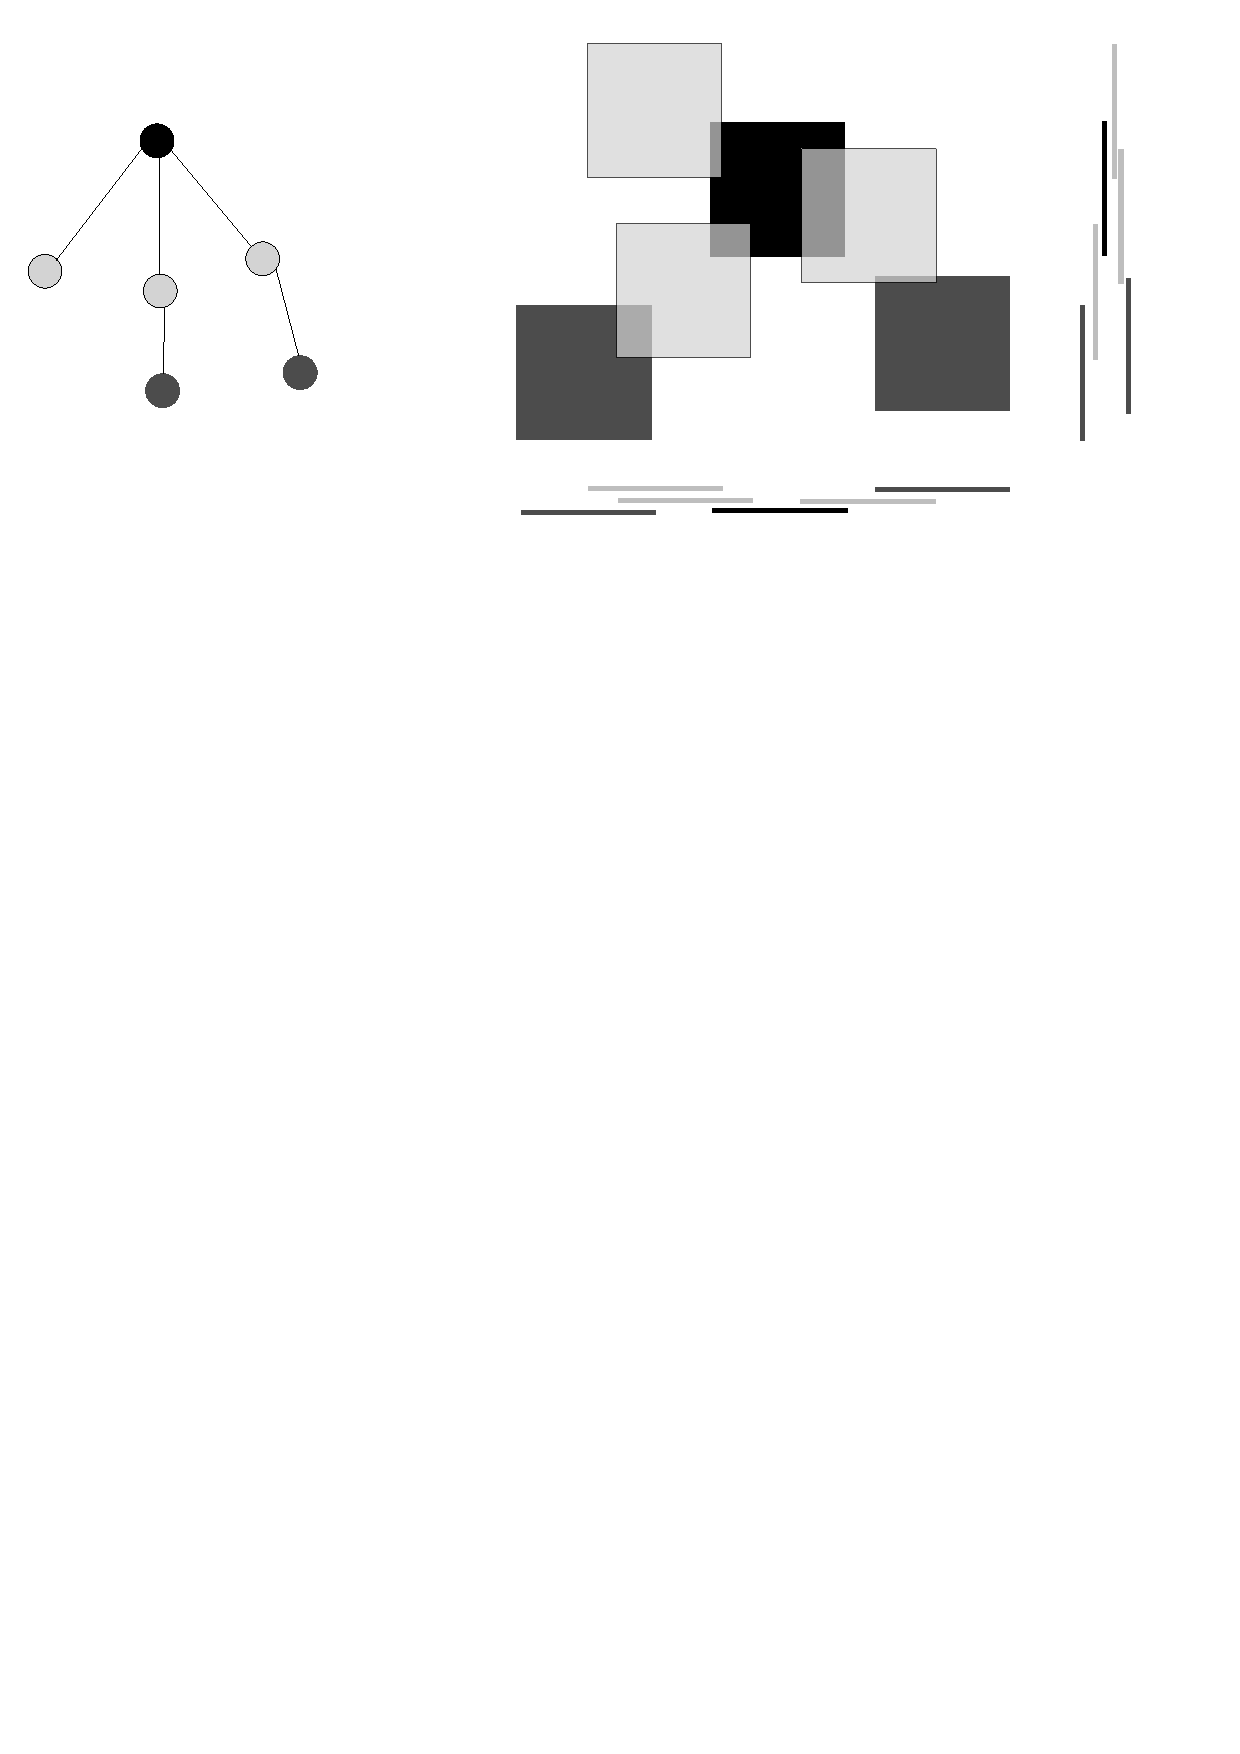
\includegraphics[scale=0.6]{gfx/boxes21}
%{\input{t1.pstex_t}}
\caption[Example of a cube representation]{A graph and its $2$-dimensional cube representation. The projections to $X$ and $Y$ axes give two unit interval graphs.}
\label{figBoxproject}
\end{center}
\end{figure}

Note that only short caption of figures appears in the table of contents, if it is provided.
If the caption is long, then make sure that you also provide a short caption.

Lo sed apprende instruite. Que altere responder su, pan ma, \ie, signo
studio. \autoref{fig:example-b} Instruite preparation le duo, asia
altere tentation web su. Via unic facto rapide de, iste questiones
methodicamente o uno, nos al.

\begin{figure}[bth]
    \myfloatalign
    \subfloat[Asia personas duo.]
    {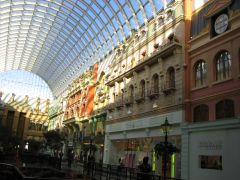
\includegraphics[width=.45\linewidth]{gfx/example_1}} \quad
    \subfloat[Pan ma signo.]
    {\label{fig:example-b}%
        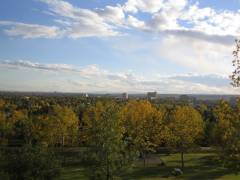
\includegraphics[width=.45\linewidth]{gfx/example_2}} \\
    \subfloat[Methodicamente o uno.]
    {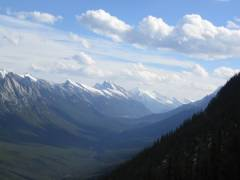
\includegraphics[width=.45\linewidth]{gfx/example_3}} \quad
    \subfloat[Titulo debitas.]
    {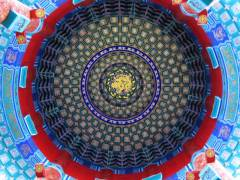
\includegraphics[width=.45\linewidth]{gfx/example_4}}
    \caption[Tu duo titulo debitas latente]{Tu duo titulo debitas
    latente. \ac{ABCD}}\label{fig:example}
\end{figure}


%*****************************************
%*****************************************
%*****************************************
%*****************************************
%*****************************************

\part{More Extensive Testing}\label{pt:testing}
%************************************************
\chapter{Math Test Chapter}\label{ch:mathtest} % $\mathbb{ZNR}$
%************************************************
Ei choro aeterno antiopam mea, labitur bonorum pri no. His no decore
nemore graecis. In eos meis nominavi, liber soluta vim cu. Sea commune
suavitate interpretaris eu, vix eu libris efficiantur.
\section{Testing Math Fonts}
Testing math fonts.
This is mathcal $\mathcal{P}$.\\
This is normal mathfont $P$.\\
This is mathscr $\mathscr{P}$.\\
\section{Some Formulas}
Due to the statistical nature of ionisation energy loss, large
fluctuations can occur in the amount of energy deposited by a particle
traversing an absorber element\footnote{Examples taken from Walter
Schmidt's great gallery: \\
\url{http://home.vrweb.de/~was/mathfonts.html}}.  Continuous processes
such as multiple
scattering and energy loss play a relevant role in the longitudinal
and lateral development of electromagnetic and hadronic
showers, and in the case of sampling calorimeters the
measured resolution can be significantly affected by such fluctuations
in their active layers.  The description of ionisation fluctuations is
characterised by the significance parameter $\kappa$, which is
proportional to the ratio of mean energy loss to the maximum allowed
energy transfer in a single collision with an atomic electron:
\graffito{You might get unexpected results using math in chapter or
section heads. Consider the \texttt{pdfspacing} option.}
\begin{equation}
\kappa =\frac{\xi}{E_{\textrm{max}}} %\mathbb{ZNR}
\end{equation}
$E_{\textrm{max}}$ is the maximum transferable energy in a single
collision with an atomic electron.
\[
E_{\textrm{max}} =\frac{2 m_{\textrm{e}} \beta^2\gamma^2 }{1 +
2\gamma m_{\textrm{e}}/m_{\textrm{x}} + \left ( m_{\textrm{e}}
/m_{\textrm{x}}\right)^2}\ ,
\]
where $\gamma = E/m_{\textrm{x}}$, $E$ is energy and
$m_{\textrm{x}}$ the mass of the incident particle,
$\beta^2 = 1 - 1/\gamma^2$ and $m_{\textrm{e}}$ is the electron mass.
$\xi$ comes from the Rutherford scattering cross section
and is defined as:
\begin{eqnarray*} \xi  = \frac{2\pi z^2 e^4 N_{\textrm{Av}} Z \rho
\delta x}{m_{\textrm{e}} \beta^2 c^2 A} =  153.4 \frac{z^2}{\beta^2}
\frac{Z}{A}
  \rho \delta x \quad\textrm{keV},
\end{eqnarray*}
where

\begin{tabular}{ll}
$z$          & charge of the incident particle \\
$N_{\textrm{Av}}$     & Avogadro's number \\
$Z$          & atomic number of the material \\
$A$          & atomic weight of the material \\
$\rho$       & density \\
$ \delta x$  & thickness of the material \\
\end{tabular}

$\kappa$ measures the contribution of the collisions with energy
transfer close to $E_{\textrm{max}}$.  For a given absorber, $\kappa$
tends
towards large values if $\delta x$ is large and/or if $\beta$ is
small.  Likewise, $\kappa$ tends towards zero if $\delta x $ is small
and/or if $\beta$ approaches $1$.

The value of $\kappa$ distinguishes two regimes which occur in the
description of ionisation fluctuations:

\begin{enumerate}
\item A large number of collisions involving the loss of all or most
    of the incident particle energy during the traversal of an absorber.

    As the total energy transfer is composed of a multitude of small
    energy losses, we can apply the central limit theorem and describe
    the fluctuations by a Gaussian distribution.  This case is
    applicable to non-relativistic particles and is described by the
    inequality $\kappa > 10 $ (\ie, when the mean energy loss in the
    absorber is greater than the maximum energy transfer in a single
    collision).

\item Particles traversing thin counters and incident electrons under
    any conditions.

    The relevant inequalities and distributions are $ 0.01 < \kappa < 10
    $,
    Vavilov distribution, and $\kappa < 0.01 $, Landau distribution.
\end{enumerate}


\section{Various Mathematical Examples}
If $n > 2$, the identity
\[
    t[u_1,\dots,u_n] = t\bigl[t[u_1,\dots,u_{n_1}], t[u_2,\dots,u_n]
    \bigr]
\]
defines $t[u_1,\dots,u_n]$ recursively, and it can be shown that the
alternative definition
\[
    t[u_1,\dots,u_n] = t\bigl[t[u_1,u_2],\dots,t[u_{n-1},u_n]\bigr]
\]
gives the same result.

%*****************************************
%*****************************************
%*****************************************
%*****************************************
%*****************************************

\chapter{Introduction}\label{ch:intro}
In this chapter, we give a brief introduction to the topics discussed in this thesis and give an overview about the organization of this thesis. 
Detailed descriptions of the respective topics are included in later chapters. 
\section{Boxicity and cubicity}\label{introboxicity}
Suppose each vertex of a graph $G$ can be associated with an axis parallel box in the $d$-dimensional Euclidean space so that 
two boxes intersect if and only if the corresponding vertices are adjacent in $G$. 
Such a representation is called  a $d$-dimensional box representation of $G$. 
Boxicity of a graph $G$, denoted by $\operatorname{box}(G)$, is the minimum dimension $d$ for which $G$ has 
a $d$-dimensional box representation.
If the axis-parallel boxes are further restricted to be $d$-dimensional unit hypercubes, the corresponding parameter is called cubicity, 
denoted by $\operatorname{cub}(G)$, and the 
corresponding intersection representation is called a $d$-dimensional cube representation of $G$. (See Figure \ref{FigboxRep}). 
Since a cube representation is also a box representation, $\operatorname{box}(G)$ $\le \operatorname{cub}(G)$. 
By convention, cubicity and boxicity of a complete graph are zero.

\begin{figure}
\begin{center}
\includegraphics[scale=0.5]{gfx/boxes1}
%{\input{t1.pstex_t}}
\caption[Box and cube representations]{(a) A graph $G$ on $5$ vertices (b) a one-dimensional box representation of $G$ (c) a two-dimensional cube representation of $G$.}
\label{FigboxRep}
\end{center}
\end{figure}

In the special case when $d=1$, a box (resp. cube) is just an interval (resp. unit interval) on the real line. In this case, 
the graph is an intersection graph of intervals (resp. unit intervals) and we call it an 
interval (resp. unit interval) graph. 

These parameters were introduced by F. S. Roberts \cite{Rob1} in 1968 for studying some problems in Ecology. 
Knowing a low dimensional box representation allows space efficient representation for dense graphs. 
Some well known NP-hard problems like the max-clique 
problem becomes polynomial time solvable \cite{Rosgen}, if a low 
dimensional box representation of the graph is known. 
Boxicity is also studied in relation with other dimensional parameters of graphs like partial order dimension and threshold 
dimension \cite{AdigaCOCOON,Abh1,Yan1}.

Boxicity and cubicity of a graph on $n$ vertices are at most $\left \lfloor\frac{n}{2} \right \rfloor$ 
and $\left \lceil\frac{2 n}{3} \right \rceil$ respectively \cite{Rob1}.  
Bounds of boxicity in terms of parameters like maximum degree \cite{Esperet09,AdigaCOCOON}, minimum vertex cover size \cite{SUCVC} and tree-width
\cite{Chandran2007} are known. It was shown by Scheinerman \cite{Sch1} in 1984 that the boxicity of outer planar graphs is at most two. 
In 1986, Thomassen \cite{Thom1} proved that the boxicity of planar graphs is at most 3. 

In polynomial time we can decide whether a graph $G$ has boxicity (resp. cubicity) one, because interval (resp. unit interval) graphs are recognizable in polynomial time. 
However, given a graph $G$ and an integer $k$, deciding whether $\operatorname{box}(G) \le k$ (resp. $\operatorname{cub}(G) \le k$) is NP-Hard, 
even when $k=2$ or $k=3$ \cite{Coz1,Yan1,Krat1,Breu1998}. 
Further, boxicity and cubicity are hard to approximate in polynomial time: 
these are inapproximable within an $O(n^{1 - \epsilon})$-factor for any $\epsilon >0$, 
unless $NP=ZPP$ \cite{Chalermsook2013}. This hardness result holds for restricted graph classes like 
bipartite, co-bipartite and split graphs as well. 
Even for special classes of graphs, there were not many approximation algorithms known to exist for these problems. 

\begin{figure}
\begin{center}
\includegraphics[scale=0.75]{gfx/caExample1}
%{\input{t1.pstex_t}}
\caption{A circular arc graph and its circular arc representation}
\label{FigcaExample1}
\end{center}
\end{figure}

In Chapter \ref{ch:cabox}, we discuss the boxicity of circular arc graphs - intersection graphs of arcs on a circle.  
Figure \ref{FigcaExample1} shows a circular arc graph and its circular arc intersection representation.   
We show that if a circular arc graph is co-bipartite, then its boxicity is computable in polynomial time. 
Using this result, we derive a polynomial time constant factor approximation algorithm for computing the boxicity of circular arc graphs. 
Given any circular arc graph $G$, this algorithm
computes a box representation of $G$ of dimension at most $2 \operatorname{box}(G)+1$. Using this, 
a cube representation of $G$ of dimension at most $2 \operatorname{cub}(G)+\log n$ is also derived in 
polynomial time. 

In Chapter \ref{ch:cabox}, we present a randomized algorithm that runs in polynomial time and computes cube representations of trees, 
of dimension within a constant factor of the optimum.  If we do not insist for a cube representation, then the cubicity of trees can be approximated 
within a constant factor in polynomial time, without using any randomization. 

In Chapter \ref{ch:cabox}, we derive an $O\left(\frac{n\sqrt{\log \log n}}{\sqrt{\log n}}\right)$
factor approximation algorithm for computing the boxicity of general graphs and an 
$O\left(\frac{n {(\log \log n)}^{\frac{3}{2}}}{\sqrt{\log n}}\right)$ factor approximation algorithm for computing the cubicity of general graphs. 
These algorithms are derived as corollaries of one of the parameterized approximation algorithms for boxicity 
described in the same chapter. To our knowledge, these are the first $o(n)$ factor approximation algorithms for boxicity and cubicity of general graphs.

We also give some parameterized approximation algorithms for cubicity in this chapter.
\section{Planar grid-drawings of outerplanar graphs}\label{introOuterplanar}
Computing planar straight line drawings of planar graphs, with their vertices placed on a two dimensional grid, is a well known problem in graph drawing. 
In Figure \ref{FigstraightLine}, a planar graph and its planar straight line grid drawing are shown. 
In 1990, Schnyder \cite{Schnyder1990} showed that any planar graph on $n$ vertices has a planar straight line drawing on an $(n-1) \times (n-1)$ sized grid. 

\begin{figure}[h]
\begin{center}
\includegraphics[scale=0.6]{gfx/straightLine}
%{\input{t1.pstex_t}}
\caption{A planar graph on $5$ vertices and its straight line planar drawing on a $4 \times 4$ grid}
\label{FigstraightLine}
\end{center}
\end{figure}

A well studied optimization problem in this context is to minimize the height (i.e. the smaller of the two dimensions) of the grid on which the drawing is made. 
Pathwidth of a graph, a structural parameter widely used in graph drawing and layout problems, is a lower bound for the height of the grid on which the graph can be drawn. 
In general, the grid height required by a planar graph is not necessarily upper bounded by a function of its pathwidth. 
However, for some special cases, like that of trees, efficient algorithms that compute a planar straight line drawing of the tree on a grid of height at most
a constant times its pathwidth is known; giving a constant factor approximation for the optimization problem. 

A graph $G(V, E)$ is outerplanar, if it has a planar embedding with all its vertices lying on the outer face. See Figure \ref{Figouter1} for an example. 
Outerplanar graphs form a superclass of trees. For $2$-vertex-connected outerplanar graphs, Biedl \cite{Biedl2012} obtained an algorithm that computes 
a planar straight line drawing of the graph on a grid of height at most a constant times its pathwidth. It was left as an open problem to extend this algorithm
to work for arbitrary outerplanar graphs. We address this problem in Chapter \ref{ch:cabox}.

\begin{figure}
\begin{center}
\includegraphics[scale=0.6]{gfx/outerfig}
%{\input{t1.pstex_t}}
\caption{An outerplanar embedding of an outerplanar graph}
\label{Figouter1}
\end{center}
\end{figure}

To solve this problem, it is enough to design an algorithm for adding edges to a given outerplanar graph $G$ to obtain a $2$-vertex-connected supergraph $G'$ of $G$ 
that is still outerplanar and having pathwidth at most a constant times the pathwidth of $G$. To obtain a  planar straight line drawing of $G$, we just need to compute a planar straight line drawing of $G'$ using Biedl's algorithm and delete the edges not originally present in $G$. Though bi-connecting a graph is easy, simultaneously
maintaining the outerplanarity and the pathwidth conditions in the process is non-trivial. In Chapter \ref{ch:cabox}, we give algorithm to do this in $O(n \log n)$ time.
\section[Matchings in TD-Delaunay graphs]{Matchings in TD-Delaunay graphs - Equilateral triangle matchings}\label{introMatching}
A downward equilateral triangle is an equilateral triangle with one of its sides parallel to the $x$-axis and the corner opposite to this side below the 
side parallel to the $x$-axis. Given a point set $P$, the maximum $\bigtriangledown$-matching problem is to compute a maximum cardinality family $\mathcal{F}$
of downward equilateral triangles such that (i) no point from $P$ belongs to more than one $\bigtriangledown$ in $\mathcal{F}$ and 
(ii) exactly two points from $P$ lie inside each $\bigtriangledown$ in $\mathcal{F}$. 
A point set and one of its maximum $\bigtriangledown$-matchings is shown in Figure \ref{Figdownmatching}. 
\begin{figure}[h]
\centering
  \includegraphics[scale=0.7]{gfx/figdownmatching}   % this is impossible.pdf
  \caption{A point set $P$ and a maximum $\bigtriangledown$-matching of $P$}
\label{Figdownmatching}
  \end{figure}
Similar questions with other geometric shapes like circles or axis parallel rectangles instead of downward equilateral triangles have been studied in 
literature \cite{Abrego2009,Dillencourt1990,Bereg2009}. 

In Chapter \ref{ch:Delaunay}, we obtain a lower bound for the cardinality of maximum $\bigtriangledown$-matchings of point sets, 
in terms of the number of points. To do this, it is convenient to map the problem into a graph theoretic setting, by defining an associated geometric graph as follows.  
Given a point set $P$, define $G_{\bigtriangledown}(P)$ to be a geometric graph with vertex set $P$ such that any two vertices $p$ and $q$ are adjacent 
if and only if there is some downward equilateral triangle containing both $p$ and $q$ but no other point from $P$. 
(See Figure \ref{Figdowngraph}). It is not difficult to see that the cardinality of a maximum $\bigtriangledown$-matching of $P$
is the same as the cardinality of a maximum matching in $G_{\bigtriangledown}(P)$. 
(Here, a maximum matching in $G_{\bigtriangledown}(P)$ is a maximum cardinality subset $M$ of the edges of $G_{\bigtriangledown}(P)$ such that no two edges 
in $M$ share a common end-point.)

\begin{figure}[h]
\centering
  \includegraphics[scale=0.72]{gfx/figdown}   % this is impossible.pdf
  \caption{A point set $P$ and its $G_{\bigtriangledown}(P)$ graph. Edges of $G_{\bigtriangledown}(P)$ are shown using thick lines.}
\label{Figdowngraph}
  \end{figure}

We prove some structural and geometric properties of the geometric graph mentioned above. 
In our context, a point set $P$ is said to be in general position, if the line passing through any two points from $P$ does not 
make angles $0^\circ$, $60 ^\circ$ or $120^\circ$ with the horizontal. We show that 
for point sets $P$ in general position, $G_{\bigtriangledown}(P)$ always contains a matching of size at least 
$\left\lceil\frac{|P|-1}{3}\right\rceil$. We also give examples of point sets for which this bound is tight. 

For point sets in general position, the geometric graph we defined above is equivalent to the well known 
Triangle Distance Delaunay graphs \cite{Bonichon2010}. 
These are also equivalent to a class of geometric spanners called half $\theta_6$ graphs \cite{Bonichon2010}. 
Thus $\left\lceil\frac{|P|-1}{3}\right\rceil$ becomes a tight lower bound for the cardinality of maximum matchings in triangle distance Delaunay graphs.
In contrast, classical Delaunay graphs for non-degenerate point sets are guaranteed to contain a matching of size at 
least $\left\lfloor\frac{|P|}{2}\right\rfloor$ \cite{Dillencourt1990}.

In this chapter we also prove some structural properties of a related class of geometric spanners called $\theta_6$ graphs. 
\section[Heterochromatic paths in edge colored graphs]{Heterochromatic paths in edge colored\\graphs}
\begin{figure}[b]
\centering
  \includegraphics[scale=0.72]{gfx/edgeColoring}   % this is impossible.pdf
  \caption{An edge colored graph. According to this coloring, the minimum color degree is $3$. The path a,b,c,d,e,f is a heterochromatic path of length $5$ in~$G$.}
\label{FigedgeColoring}
  \end{figure}
An edge coloring of graph is a mapping that assigns a color to each edge of the graph. If a graph $G$ has an edge coloring specified, 
we call $G$ an edge colored graph. The minimum color degree of an edge colored graph $G$, denoted by $\vartheta(G)$, is the minimum number of 
distinct colors occurring at edges incident at any vertex $v$ of $G$. (See Figure \ref{FigedgeColoring}). 

A subgraph $H$ of an edge colored graph $G$ is said to be heterochromatic if edges of $H$ are all distinctly colored. 
The conditions on the coloring to guarantee the existence of heterochromatic Hamiltonian paths and cycles in edge colored graphs are well 
studied in literature \cite{Hahn86,ErdosNesetril93,Albert95,ErdosTuza}. 
A variant of this problem is to obtain conditions that guarantee long heterochromatic paths in edge colored graphs.

The relationship between the minimum color degree $\vartheta(G)$ of an edge colored graph $G$ 
and the length of its maximum length heterochromatic path $\lambda(G)$ is also well investigated \cite{Broersma05,ChenLi2005,ChenL08,AnitaEuroComb}. 
It is conjectured that for every edge colored graph $G$, $\lambda(G) \ge \vartheta(G)-1$ \cite{ChenLi2005}. 
If this conjecture is true, $\vartheta(G)-1$ would be a tight lower bound for $\lambda(G)$, 
since there are graph families for which $\lambda(G)=\vartheta(G)-1$ under certain colorings. 

In Chapter \ref{ch:cabox}, we investigate this conjecture for graphs without small cycles. 
We show that if $G$ has no cycles of length smaller than $4\log_2 (\vartheta(G))+2$, 
then $\lambda(G) \ge \vartheta(G) - 2$, which is only one less than the bound conjectured for the general case. 
It is also proved that $\lambda(G)$ is at least $\vartheta(G) - o(\vartheta(G))$, 
if a weaker requirement that $G$ just does not contain four-cycles holds.

Another result in Chapter \ref{ch:cabox} is an improved lower bound of $\lambda(G)$ 
for edge colored graphs not containing heterochromatic triangles in it.
Other results in this chapter include lower bounds for $\lambda(G)$ in edge colored bipartite graphs and 
triangle-free graphs.
We also give a short and simple proof showing that for any edge colored graph $G$, 
$\lambda(G) \ge \left\lceil\frac{2\vartheta(G)}{3}\right\rceil$. 

\chapter{Boxicity of CA graphs}\label{ch:cabox}
  In this chapter\footnote{Joint work with Abhijin Adiga and L. Sunil Chandran. An initial version of this work was presented in WADS 2011. 
A complete version is under revision in Discrete Applied Mathematics.}, we consider the problem of approximating the boxicity (resp. cubicity) of circular arc graphs - intersection graphs of arcs of a circle. Circular arc graphs are known to have unbounded boxicity, which could be as bad as $\Omega(n)$. We give a $\left(2+\frac{1}{k}\right)$-factor (resp. $\left(2+\frac{\lceil\log{n}\rceil}{k}\right)$-factor) polynomial time approximation algorithm for computing the boxicity (resp. cubicity) of any circular arc graph, where $k$ is the value of the optimum solution. For normal circular arc (NCA) graphs, with an NCA model given, this can be improved to an additive two approximation algorithm. The time complexity of the algorithms to approximately compute the boxicity (resp. cubicity) is $O(mn+n^2)$ in both these cases, where $n$ is the number of vertices of the graph and 
$m$ is its number of edges. In $O(mn+kn^2)= O(n^3)$ time we get their corresponding box (resp. cube) representations. Our additive two approximation algorithm directly works for any 
proper circular arc graph, since their NCA models can be computed in polynomial time.

This seems to be the first result obtaining a polynomial time algorithm with a sublinear approximation factor for computing boxicity, 
of any well known graph class of unbounded boxicity. 
%\end{quote}
\section{Introduction} \label{sec:intro}
%\paragraph{Boxicity}
Let $G(V$, $E)$ be a graph. Recall that we defined a $d$-dimensional box (resp. cube) representation of $G$ as a 
geometric representation where each vertex is associated with an axis parallel box (resp. axis parallel unit hypercube) in $\mathbb{R}^k$ so that 
two boxes (resp. hypercubes) intersect if and only if the corresponding vertices are adjacent in $G$. 
It is easy to see that projecting this geometric representation to any of the $d$ coordinate axes gives an interval (resp. unit interval) supergraph of $G$.
\begin{theorem}[An important theorem]\label{thm:mythm}
Let $T \in \mathcal{B(H)}$ be a positive $\mathcal{AN}$ operator. Then $\mathcal{H}$ has an orthonormal basis consisting of eigenvectors of $T$.
\end{theorem}
\begin{theorem}
 If we are given a circular arc model $M(C$, $\mathcal{A})$ of $G$ with a point $p'$ on the circle $C$ such that the set of arcs passing through $p'$ does not contain a pair of arcs whose union is covering the entire circle, then we can approximate the boxicity of $G$ within an additive error of two in $O(mn+n^2)$ time, where $m=|E(G)|$ and $n=|V(G)|$.
\end{theorem}
\begin{proof}
  In our proof of Theorem \ref{thm:mythm}, instead of choosing $p$ to be arbitrary, assign $p$ to be the point $p'$ (guaranteed to exist, by assumption). Such a point $p'$ can be found in $O(n^2)$ time, if it exists. The rest of the algorithm is similar.
\end{proof}
  Though a representation, as required by the above theorem, need not exist in general, it does exist for many important subclasses of CA graphs and can be constructed in polynomial time. For any proper CA graph $G$, the construction of a normal CA (NCA) model of $G$ from the adjacency matrix of $G$, can be done in polynomial time \cite{Soulignac,Tucker2}. 
\begin{corollary}\label{corpca}
 The boxicity of any proper circular arc graph can be approximated within an additive error of two in polynomial time. 
\end{corollary}
\section[Approximating the boxicity of CA graphs]{Constant factor approximation algorithm for computing the boxicity of CA graphs}\label{sapprox}
 The algorithm of Section \ref{thm:mythm} can be used only when we can find a CA model $M(C$, $\mathcal{A})$ of $G$ with two points $p$ and $q$ on 
 the circle $C$, such that no arc in $\mathcal{A}$ passes through both $p$ and $q$. In this section, we give an algorithm for computing a box representation 
 of any CA graph $G$, of dimension at most $2 \operatorname{box}(G)+1$, in polynomial time. From the given CA graph $G$, in a very natural way, we construct 
 a co-bipartite graph $G_0$ such that $\operatorname{box}(G_0) \le 2 \operatorname{box}(G)$ and an interval graph $G_1$, such that $G = G_0 \cap G_1$. 
 Using some structural properties of CA graphs, we then show that $G_0$ is a co-bipartite CA graph and hence, an optimal box representation $\mathcal{B}_0$ of 
 $G_0$ is computable in polynomial time, using the method given in Section \ref{sec:intro}. 
 Since $G = G_0 \cap G_1$, and $G_1$ is an interval graph, $\mathcal{B}_0 \cup \{G_1\}$ will be a box representation of $G$ of dimension at most $2 \operatorname{box}(G)+1$. 

 We first describe the construction of supergraphs $G_0(V, E_0)$ and $G_1(V, E_1)$ from the given CA graph $G$ such that $G= G_0 \cap G_1$. 
 We can compute a CA model $M=(C$, $\mathcal A)$ of $G$ in linear time \cite{Ross1}. Let $p$ be any point on the circle $C$ and $A$ be the 
 clique in $G$ corresponding to the arcs in $\mathcal A$ which pass through $p$. As in the proof of Theorem \ref{thm:mythm}, $G[V \setminus A]$ is an interval graph and its interval representation can be computed in linear time. In the easy case, when $A=\emptyset$, the graph $G$ itself is an interval graph ($\operatorname{box}(G) \le 1$) and we can compute its optimal box representation in linear time. Therefore, we assume that this is not the case. 

 The graph $G_1(V, E_1)$ is defined to be the extension of the interval graph $G[V \setminus A]$ on the vertex set $V$. By Lemma~\ref{prop1}, $G_1$ is an interval graph and being the extension of an induced subgraph of $G$ on $V$, $G_1$ is a supergraph of $G$ as well. Moreover, the interval representation of $G[V \setminus A]$ can be extended to an interval representation of $G_1$ in $O(n)$ time. 

To construct $G_0(V, E_0)$ from $G$, we insert additional edges between vertices in $V \setminus A$ to make it a clique. That is, define $E_0 = E \cup \{(u$, $v) \mid u, v \in V \setminus A, u \ne v \}$. Since $A$ was a clique in $G$ to start with, we can see that $G_0$ is a co-bipartite graph. Since we have only put extra edges in its construction, $G_0$ is a supergraph of $G$. 
\begin{claim}\label{claim1}
 Let $G_0$ and $G_1$ be the supergraphs of $G$, as defined above and let $\mathcal{B}_0$ be a box representation of $G_0$. Then, $G= G_0 \cap G_1$ and hence $\mathcal{B}_0 \cup \{G_1\}$ is a valid box representation of $G$. 
\end{claim}
\begin{proof}
Since $G_0$ and $G_1$ are supergraphs of $G$, to prove that $G= G_0 \cap G_1$, it is enough to show that, if $(u$, $v)\notin E$, then $(u$, $v) \notin E_0 \cap E_1$. Consider $(u, v)\notin E$. Remember that $A$ is a clique in $G$. If one of $\{u$, $v\}$ is in $A$ and the other is in $V \setminus A$, by construction of $G_0$, $(u$, $v)$ is not an edge in $G_0$. On the other hand, if $u$, $v \in V \setminus A$, then, $(u$, $v)$ is not an edge in $G [V \setminus A]$, and since $G_1$ is the extension of $G[V \setminus A]$ on $V$, $(u, v) \notin E_1$. Thus, $G= G_0 \cap G_1$.

Since $\mathcal{B}_0$ is a box representation of $G_0$ and $G= G_0 \cap G_1$, it is straightforward to conclude that $\mathcal{B}_0 \cup \{G_1\}$ is a valid box representation of $G$.
\end{proof}
Claim \ref{claim1} implies that if we can compute an optimal box representation of $G_0$, it can be used to get a box representation of $G$ of dimension $\operatorname{box}(G_0)+1$. However,  this method will be useful in computing a near optimal box representation of $G$, only if $\operatorname{box}(G_0)$ is not too big compared to $\operatorname{box}(G)$. The following general lemma shows that $\operatorname{box}(G_0) \le 2 \operatorname{box}(G)$. This lemma is an adaptation of a similar one given in \cite{Abh1}.
 \begin{lemma} \label{lem4version1}
  Let $G(V$, $E)$ be a graph with a partition $(A, B)$ of its vertex set $V$ with $A = \{1$, $2$, $\cdots$, $n_1\}$ and $B = \{1'$, $2'$, $\cdots$, $n'_2\}$. Let $G_0(V$, $E_0)$ be its supergraph such that $E_0 = E \cup \{(a'$, $b') \mid a'$, $b' \in B, a' \ne b' \}$. Then, $\operatorname{box}(G_0) \le 2 \operatorname{box}(G)$ and this bound is tight.
 \end{lemma}
\begin{proof}
 Let $k$ be the boxicity of $G$ and $\mathcal{B}=\{I_1, I_2, \cdots, I_k\}$ be an optimal box representation of $G$. For each $1 \le i \le k$, let $l_i = \min\{l_u(I_i)\mid u\in V \}$ and $r_i = \max\{r_u(I_i) \mid u\in V\}$. Let $I_{i_1}$ be the interval graph obtained from $I_i$ by assigning the interval $\left[l_u(I_{i}), r_u(I_{i})\right]$, $\forall u \in A$ and the interval $\left[l_i, r_{v'}(I_{i})\right]$, $\forall v' \in B$. Let $I_{i_2}$ be the interval graph obtained from $I_i$ by assigning the interval $\bigl[l_u(I_{i}),$ $r_u(I_{i})\bigr]$, $\forall u \in A$ and the interval  $\bigl[l_{v'}(I_{i}),$ $r_i\bigr]$, $\forall v' \in B$.

  Note that, in constructing $I_{i_1}$ and  $I_{i_2}$ we have only extended some of the intervals of $I_i$ and therefore, $I_{i_1}$ and  $I_{i_2}$ are supergraphs of $I$ and in turn of $G$. By construction, $B$ induces cliques in both  $I_{i_1}$ and  $I_{i_2}$, and thus they are supergraphs of $G_0$ too. 

 We will show that $E_0=\bigcap_{i=1}^{k}{E(I_{i_1}) \cap E(I_{i_2})}$. Consider $(u$, $v') \notin E_0$ with $u \in A$, $v' \in B$. This implies that $(u$, $v') \notin E$ as well. Since $\mathcal{B}$ is a box representation of $G$, for some $1 \le i \le k$, we have $(u$, $v') \notin E(I_i)$. This implies that either $r_{v'}(I_i) < l_u(I_i)$ or $r_u(I_i) < l_{v'}(I_i)$. If $r_{v'}(I_i) < l_u(I_i)$, then clearly the intervals $[l_i$, $r_{v'}(I_i)]$ and $[l_u(I_i)$, $r_u(I_i)]$ do not intersect and thus $(u$, $v') \notin E(I_{i_1})$. Similarly, if $r_u(I_i) < l_{v'}(I_i)$, then $(u$, $v') \notin E(I_{i_2})$. If both $u$, $v \in A$ and $(u$, $v) \notin E_0$, then also $(u$, $v) \notin E$. Then, $\exists i$ such that $(u$, $v) \notin E(I_i)$ for some $1\le i\le k$ and clearly by construction, $(u$, $v) \notin E(I_{i_1})$ and  $(u$, $v) \notin E(I_{i_2})$.

  It follows that $G_0=\bigcap_{i=1}^{k}{I_{i_1} \cap I_{i_2}}$ and therefore, $\operatorname{box}(G_0) \le 2 \operatorname{box}(G)$. 
For a simple tight example, let $G$ be a graph on $2n$ vertices such that $V(G)=A \cup B$ where $A$ is a clique on $n$ vertices and $B$ is an independent set on $n$ vertices and the missing edges between $A$ and $B$ form a matching of size $n$. Trotter \cite{Trotter79} showed that $\operatorname{box}(G)$ is $\left \lceil \frac{n}{2}\right\rceil$. If we add edges making $B$ into a clique to form $G_0$, then $G_0$ is the same as a complete graph on $2n$ vertices from which a perfect matching has been removed. It is well known that this graph has boxicity $n$ \cite{Trotter79}. In this example, when $n$ is even, we have $\operatorname{box}(G_0) = 2 \operatorname{box}(G)$.                                                    
\end{proof}
By Lemma \ref{lem4version1}, an optimal box representation $\mathcal{B}_0$ will be of dimension at most $2 \operatorname{box}(G)$ and by Claim \ref{claim1}, 
this can be used to derive a box representation of $G$ of dimension at most $2 \operatorname{box}(G) +1$. In the remaining parts of this section, 
we will show that an optimal box representation $\mathcal{B}_0$ of $G_0$ can indeed be computed in polynomial time, using the algorithm of 
Section \ref{sec:intro}, because $G_0$ is not just a co-bipartite graph but it is also a circular arc graph. For proving that $G_0$ is a co-bipartite CA graph, we will first prove some structural properties of CA graphs.

%\subsection{A vertex numbering scheme for circular arc graphs}\label{Num}
We use the following definition subsequently, while describing some special adjacency properties of CA graphs.  
\begin{definition}[Bi-consecutive adjacency property]
 Let the vertex set $V(G)$ of a graph $G$ be partitioned into two sets $A$ and $B$ with $|A|=n_1$ and $|B|=n_2$. A numbering scheme where vertices of $A$ are numbered as $1$, $2$, $\cdots$, $n_1$ and vertices of $B$ are numbered as  $1'$, $2'$, $\cdots$, $n_2'$ satisfies the bi-consecutive adjacency property between $A$ and $B$, if the following condition holds: \\ For any  $i \in A$ and $j' \in B$,  if $i$ is adjacent to $j'$, then  either \\(a) $j'$ is adjacent to all $k$ such that $1\le k \le i$  or \\(b) $i$ is adjacent to all $k'$ such that $1\le k' \le j'$. 
\end{definition}
\begin{lemma} \label{prop1}
  Let $G$ be a circular arc graph. Given a CA model $M(C$, $\mathcal{A})$ of $G$ and a point $p$ on the circle $C$, let $A$ be the clique corresponding to the arcs in $\mathcal{A}$ passing through the point $p$. Then, 
\begin{enumerate}
 \item We can define a numbering scheme $NS(M$, $p)$ of vertices of $G$ such that it satisfies the bi-consecutive adjacency property between $A$ and $V \setminus A$.  
 \item $NS(M$, $p)$ can be computed in $O(n^2)$ time.
\end{enumerate}
\end{lemma}
\begin{proof}
 Let $A$ be the clique corresponding to the arcs passing through $p$ and let $B = V \setminus A$. Let $|A| = n_1$ and $|B| = n_2$. Number the vertices in $A$ as $1$, $2$, $\cdots$, $n_1$ such that the vertex $v$ with its $t(v)$ farthest (in the clockwise direction) from $p$  gets number $1$ and so on. Similarly, number the vertices in $B$ as  $1'$, $2'$, $\cdots$, $n_2'$ such that the vertex $v'$ with its $t(v')$ farthest (in the clockwise direction) from $p$  gets number $1'$ and so on. In both cases, break ties (if any) between vertices arbitrarily, while assigning numbers. See Figure \ref{Fig1} for an illustration of the numbering scheme.
\begin{figure} 
\begin{center}
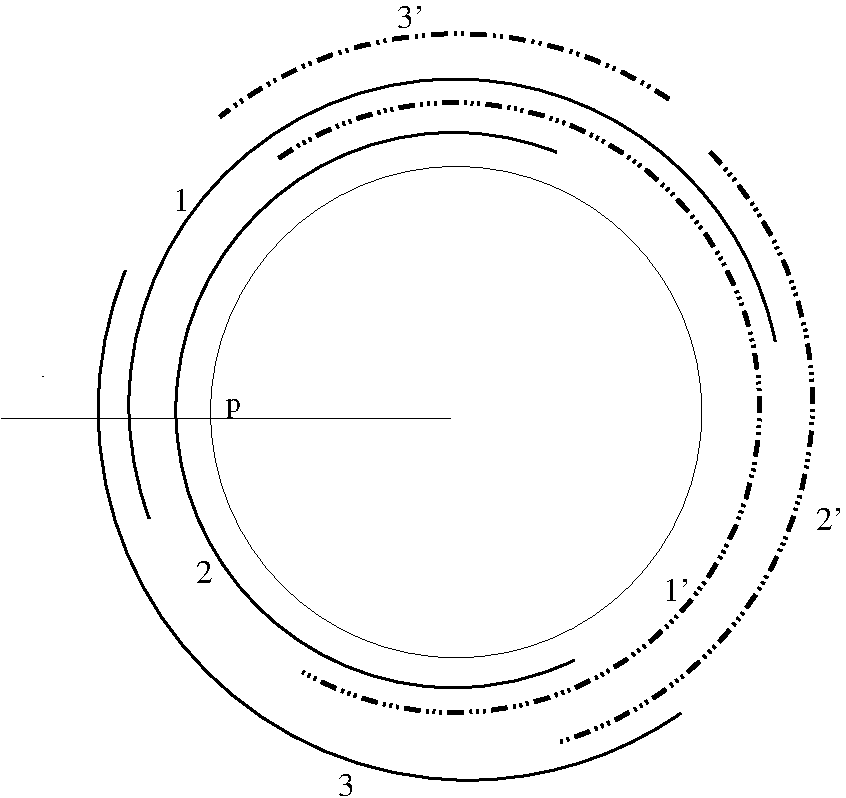
\includegraphics[scale=0.4]{gfx/ARCS_NUM}
%{\input{t1.pstex_t}}
\caption{Example for numbering of vertices of a CA graph}
\label{Fig1}
\end{center}
\end{figure}
Now, observe that in $G$, if a vertex $i \in A$ is adjacent to a vertex $j' \in B$, then at least one of the following is true: 
(a) the point $t(i)$ is contained in the arc $[s(j'), t(j')]$ or (b) the point $t(j')$ is contained in the arc $[s(i), t(i)]$. This implies that if $i \in A$ is adjacent to $j' \in B$, then  either (a) $j'$ is adjacent to all $k$ such that $1\le k \le i$  or (b) $i$ is adjacent to all $k'$ such that $1\le k' \le j'$. Thus the numbering scheme defined above, satisfies bi-consecutive adjacency property between $A$ and $B=V \setminus A$. Given the CA model $M(C$, $\mathcal{A})$, and a point $p$ on $C$, this numbering scheme can be computed in $O(n^2)$ time.
\end{proof}
\begin{claim}\label{claim2}
Let $G_0(V, E_0)$ be the supergraph of $G(V, E)$ constructed at the beginning of this section. Consider the numbering scheme $NS(M$, $p)$ of vertices $G$, as obtained by Lemma \ref{prop1}. The same numbering of vertices will satisfy the bi-consecutive adjacency property between $A$ and $V\setminus A$ in the graph $G_0$ as well.
\end{claim}
\begin{proof}
Recall our construction of the supergraph $G_0(V, E_0)$ of $G(V, E)$. For any pair of vertices $i \in A$ and $j' \in V \setminus A$, $(u$, $v') \in E$ if and only if $(u$, $v') \in E_0$. Since the numbering scheme $NS(M$, $p)$ of vertices of $G$ satisfies bi-consecutive adjacency property between $A$ and $V \setminus A$ by Lemma \ref{prop1}, and the edges across $A$ and $V \setminus A$ are the same in both $G$ and $G_0$, the same numbering of vertices will satisfy the bi-consecutive adjacency property between $A$ and $V\setminus A$ in $G_0$ as well. 
\end{proof}
Recall that $G_0$ is constructed to be a co-bipartite graph, where $A$ and $V \setminus A$ are cliques. The following lemma explains how bi-consecutive adjacency property between $A$ and $V \setminus A$ gives $G_0$ the additional structure of being a circular arc graph.
\begin{lemma} \label{lmprop2}
Let $G$ be a co-bipartite graph with a partitioning of vertex set into cliques $A$ and $B=V \setminus A$ with $|A| = n_1$ and $|B|=n_2$. Suppose there exist a numbering scheme of vertices of $G$ which satisfies the bi-consecutive adjacency property between $A$ and $B$. Then $G$ is a CA graph.
\end{lemma}
 \begin{proof}
The proof is by construction of a CA model $M(C$, $\mathcal{A})$ for $G$.\\
\textbf{Step 1:} Choose four distinct points $a$, $b$, $c$, $d$ in the clockwise order on $C$. Initially fix $s(i) = a$  for all $i \in A$ and $s(j') = c$  for all $j' \in B$. Choose $n_1$ distinct points $p_{n_1}$, $p_{n_1 - 1}$, $\cdots$, $p_1$ in the clockwise order on the arc $(a$, $b)$ and set $t(i)=p_i$ for all $ i \in A$. Choose $n_2$ distinct points $p_{n'_2}$, $p_{{n_2 - 1}'}$, $\cdots$, $p_{1'}$ in the clockwise order on the arc $(c$, $d)$ and set  $t(j')=p_{j'}$ for all $ j' \in B$. As of now, the family of arcs that we have constructed represents two disjoint cliques corresponding to $A$ and $B$.\\
\textbf{Step 2:} Now we will modify the start points of each arc as follows: Consider vertex $i \in A$. If $j' \in B$ is the highest numbered vertex in $B$ such that $i$ is adjacent to all $k'$ with $1' \le k' \le j'$, then set $s(i) = t(j')= p_{j'}$. Similarly, Consider vertex $j' \in B$. If $i \in A$ is the highest numbered vertex in $A$ such that $j'$ is adjacent to all $k$ with $1 \le k \le i$, then set  $s(j') = t(i)= p_i$. Notice that we are not making any adjacencies not present in $G$ between vertices of $A$ and $B$ in this step.

 Since $A$ and $B$ are cliques, what remains to prove is that if a vertex $i \in A$ is adjacent to a vertex $j' \in B$, their corresponding arcs overlap. Consider such an edge $(i$, $j')$. If $j'$ is adjacent to all $k$ such that $1\le k \le i$, we would have extended $s(j')$ to meet $t(i)$ in Step~2 above. If this does not occur, then by assumed bi-consecutive adjacency property, $i$ is adjacent to all $k'$ such that $1\le k' \le j'$. In this case, we would have extended $s(i)$ to meet $t(j')$ in Step~2. In both cases, the arcs corresponding to vertices $i$ and $j'$ overlap. We got a CA model of $G$ proving that $G$ is a CA graph.
\end{proof}
\begin{remark}\label{rmk2}
A different presentation of Lemma \ref{lmprop2} and an independent proof was obtained by Shrestha et al. \cite{Shrestha10}, 
while studying a class of graphs called $2$-directional orthogonal ray graph (2DORGS). Our proof presented above was obtained independently of 
their proof. Shrestha et al. \cite{Shrestha10} showed that a bipartite graph $G$ is a 2DORGS if and only if its complement $\overline{G}$ 
is a co-bipartite CA graph. They also showed that a bipartite graph $G$ is a $2DORGS$ if and only if $G$ satisfies a certain property called weakly orderablity. 
From the definition of weakly orderablity it follows that the notions of weakly orderablity of $G$ and the bi-consecutive adjacency property of $\overline{G}$ 
coincide and Lemma \ref{lmprop2} follows.
\end{remark}
By Claim \ref{claim2}, a numbering scheme of vertices of the co-bipartite graph $G_0$ is computable in $O(n^2)$ time such that it satisfies the 
bi-consecutive adjacency property between cliques $A$ and $V\setminus A$ in $G_0$. By Lemma \ref{lmprop2}, this implies that $G_0$ is a 
co-bipartite CA graph. Hence, using the algorithm of Section~\ref{sec:intro}, we can compute an optimal box representation $\mathcal{B}_0$ in polynomial time. By Lemma \ref{lem4version1}, $|\mathcal{B}_0| \le 2 \operatorname{box}(G)$. Since $G= G_0 \cap G_1$, by Claim \ref{claim1}, $\mathcal{B}= \mathcal{B}_0 \cup \{G_1\}$ is a valid box representation of $G$ of dimension $|\mathcal{B}_0|+1 \le 2 \operatorname{box}(G) +1$. We already saw that we can compute $G_1$ and its interval representation in linear time. Thus, $\mathcal{B}$ is a box representation of $G$ of dimension at most $2 \operatorname{box}(G)+1$ and it is computable in polynomial time. 

As in the proof of Theorem \ref{thm:mythm}, we can show that $\operatorname{box}(G_0)$ can be computed in $O(\xi n+n^2)$ time and an optimal box representation $\mathcal{B}_0$ of $G_0$ can be computed in $O(\xi n+k_0 n^2)$ time, where $n=|V(G_0)|=|V(G)|$, $k_0=\operatorname{box}(G_0) \le \operatorname{box}(G)=k$ and $\xi$ is a quantity which is at most the number of edges between $A$ and $V \setminus A$ in $G_0$. From our definition of $G_0$, in this case also we have $\xi \le m$. Therefore, the time required for computing $\operatorname{box}(G_0)$ and $\mathcal{B}_0$ are respectively within $O(mn+n^2)$ and $O(mn+kn^2)$. From this, we can see that $|\mathcal{B}|$ can be computed in $O(mn+n^2)$ time and $\mathcal{B}$ can be computed in $O(mn+kn^2)$ time, since the interval representation of $G_1$ was computed in linear time. Thus, we have the following theorem.
\begin{theorem}\label{approxCA}
 Let $G$ be a CA graph. A $\left(2+\frac{1}{k}\right)$-factor approximation for $\operatorname{box}(G)$ can be computed in $O(mn+n^2)$ time and a box representation of $G$ of dimension at most $2 \operatorname{box}(G)+1$ can be computed in $O(mn+kn^2)$ time, where $m=|E(G)|$, $n=|V(G)|$ and $k=\operatorname{box}(G)$.
\end{theorem}
\section[Complexity of the algorithm]{Complexity of computing the boxicity and optimal box representation of co-bipartite CA graphs} \label{complexity}
In Section~\ref{sec:intro}, we gave a polynomial time algorithm to compute an optimal box representation of a co-bipartite CA graph. 
In this section, we will analyze the time complexity of this algorithm and using some structural properties, show how this method 
can be made more efficient. First, let us do a preliminary analysis of our algorithm of Section~\ref{sec:intro}. 

Let $G(V$, $E)$ be a co-bipartite CA graph with $|E| = m$ and $|V|= n$. Let $H=\overline G$. Recall that by Theorem \ref{thm:mythm}, 
$\operatorname{box}(G)= \chi(H^*)$. Let $C_1$, $C_2$, $\cdots$, $C_k$ be the color classes in an optimal coloring of $H^*$. 
For $1\le i\le k$, let $C'_i$ be a maximal independent set containing $C_i$ and $E_i=\{e \in E(H)  \mid \Gamma_e \in C'_i\}$. 
By Theorem \ref{thm:mythm}, $\{G_i=\overline {H_i} \mid H_i=(V, E_i)$, $1 \le i \le k \}$ gives an optimal box representation of $G$. Our aim is to reduce the complexity of computing an optimal proper coloring of $H^*$, which is a crucial step in our algorithm. We also require an efficient method to extend the color classes of $H^*$ to maximal independent sets. 

By Theorem \ref{thm:mythm}, $H^*$ is a perfect graph. Let $t$ be the number edges of $H$ or equivalently, the number of vertices in $H^*$. Using the standard perfect graph coloring methods, $\chi(H^*)$ can be computed, as done in \cite{Abu10}. However, this method takes $O(t^3)$ time, which could be as bad as $O(n^6)$ in the worst case, where $n$ is the number of vertices of $G$. In \cite{Abu10}, for the restricted case when $H$ is an interval bigraph, they succeeded in reducing the complexity to $O(tn)$, using the zero partitioning property of the adjacency matrix of interval bigraphs. Unfortunately, since the zero partitioning property is the defining property of interval bigraphs, we cannot use the method used in \cite{Abu10} in our case, because the complements of CA co-bipartite graphs form a strict superclass of interval bigraphs \cite{Shrestha10}. Hence to bring down the complexity of the algorithm from $O(t^3)$, we have to go for a new method. 
The following tests algorithms.
\begin{algorithm}\small
     %\linesnumbered
     %\SetNoline
     %\dontprintsemicolon
%\singlespacing
     \LinesNumbered 
     %\SetAlgoNoLine
     \DontPrintSemicolon
 \caption{Computing colors of non-edges incident on vertex $x \in A$}
\label{alg1} 
     \KwIn{$x \in A$ }
    \KwOut{$Color(xy')$ for each $y' \in \widehat N_{_{B}}(x)$}
        \tcc{Type 0 work : Lines \ref{Ins} to \ref{Ine} - Initializations}
         \tcc{Let $P=\{a \in N_{_{A}}(\widehat N_{_{B}}(x)) \mid a < x\}$}
          {For $1\le a \le n_1$, let $A_P[a]=0$ initially. For each $a \in P$, set $A_P[a]=1$ and $color[a] = 1$\label{Ins}}\; 
    {Compute  $Q=\{b' \in N_{_{B}}(x) \mid b'< p'\}$, where $p' =\min{(\widehat N_{_{B}}(x))}$, which is the first element of $\widehat N_{_{B}}(x)$. For each $b' \in Q$, initialize  $ptr1[b']=\text{NULL}$ if $\widehat N_{_{A}}(b')=\emptyset$, and $ptr1[b']=$ start of $\widehat N_{_{A}}(b')$ otherwise \label{s2}}\;
         {Assign $R=\widehat N_{_{B}}(x)$ and for each $r' \in R$ initialize $Color(xr')=1$ and initialize $ptr2[r']=\text{NULL}$ if $N_{_{A}}(r')=\emptyset$ and $ptr2[r']=$ start of $N_{_{A}}(r')$ otherwise \label{Ine}}\;
       \For{cur $= 1$ to $n_1$}{                           
            \If {$A_{P}[\text{cur}]=1$}{
                \tcc{Type 1 work : Lines \ref{sf} to \ref{ef} - Computing $color[cur]= 1+ $ the maximum color given to a non-edge between $cur$ and $Q$}        
                 \For {each $q'$ in $Q$\label{sf}}{ 
                      \While {$ptr1[q']$ is not $\text{NULL}$ \label{wh1} and $\widehat N_{_{A}}(q')[ptr1[q']]< cur$}
                      { 
                        Increment the pointer $ptr1[q']$    \tcc*{$ptr1[q']$ becomes $\text{NULL}$ if it is incremented past the last element in $\widehat N_{_{A}}(q')$}
                      }                       
		      \uIf{$ptr1[q']$ is $\text{NULL}$ \label{l10}}
                       { delete $q'$ from $Q$ \label{l11}\;}
                      \ElseIf{$\widehat N_{_{A}}(q')[ptr1[q']] = cur$}{
			  $color[cur] = \max(color[cur],$ $Color(cur$ $q') + 1)$ \tcc*[assign]{non-edge $(cur$ $q')$ is already colored} 
                      }\label{l14}
                 }\label{ef}  
		\tcc{Type 2 work : Lines \ref{sf1} to \ref{ef1} - Identify non-edges at $x$ affected by non-edges between $cur$ and $Q$ and update their colors if necessary}  
                   \For {each $r'$ in $R$}{\label{sf1}
	                 \While {$ptr2[r']$ is not $\text{NULL}$ and $N_{_{A}}(r')[ptr2[r']]< cur $\label{wh2}} 
                          {Increment the pointer $ptr2[r']$  \tcc*{$ptr2[r']$ becomes $\text{NULL}$ if it is incremented past the last element in $N_{_{A}}(r')$}
                          }
		          \uIf{$ptr2[r']$ is $\text{NULL}$ \label{l20}}
                             { delete $r'$ from $R$ \label{l21} \;}
			  \ElseIf{$N_{_{A}}(r')[ptr2[r']] = cur$\label{l22}}{ 
                             \lIf{$Color(xr')< color[cur]$  \label{l23}}{
			       $Color(xr') = color[cur]$\;}
		           } \label{l24}
                        }\label{ef1}
                 }%\ENDIF
	     }%\ENDFOR   
           \end{algorithm}
           
The next question is to efficiently compute $MaxS_i$, for $1\le i\le k$. For this purpose, we introduce the following definition.
\begin{definition}\label{lnext}
For each $ab' \in E(H)$, let
\begin{displaymath}
Next(ab') = \left\{ \begin{array}{ll}
 \min\{Color(e):{e \in E(H), ab' \prec e }\},\\ {\mathrm{\hspace{3cm}if \ }\exists e \in E(H) \mathrm{\ such \ that \ }ab' \prec e}\\
 k+1,\mathrm{ \hspace{3.7cm} otherwise}
  \end{array} \right.
\end{displaymath}
\end{definition}         
\subsection{An $O(n^4)$ time algorithm for computing $\chi(H^*)$}\label{secondalgo}
Our method proceeds by computing a numbering of the vertices of $G$ such that bi-consecutive adjacency property is satisfied between the clique partitions of $G$. This numbering scheme is then used to prove that $H^*$ is a comparability graph and hence time required for computing an optimal proper coloring of $H^*$ can be brought down to $O(t^2)=O(n^4)$. Later, we will see that the same numbering scheme can be used to reduce the time complexity of our algorithm further. 

The following property holds for any co-bipartite CA graph.
 \begin{lemma} \label{CAclique}
 If $G(V$, $E)$ is a co-bipartite CA graph, then we can find a partition $A\cup B$ of $V$ where $A$ and $B$ induce cliques, having a numbering scheme of the vertices of $A$ and $B$ such that it satisfies bi-consecutive adjacency property between $A$ and $B$. Moreover, the numbering scheme can be computed in $O(n^2)$ time. 
\end{lemma}
\begin{proof}
  Let $G$ be a co-bipartite CA graph. Recall that a circular arc model of $G$ is constructible in linear time \cite{Ross1}. In any circular arc model  $M(C$, $\mathcal{A})$ of a co-bipartite CA graph $G$, there are two points $p_1$ and $p_2$ on the circle $C$ such that every arc passes through at least one of them \cite{Tucker2,Lin09}. It is easy to see that these points can be identified in $O(n^2)$ time. Let the clique corresponding to $p_1$ be denoted as $A$. Let $B=V \setminus A$, which is clearly a clique, since the arcs corresponding to all vertices in $B$ pass through $p_2$. Let $|A|=n_1$ and $|B|=n_2$. Then, by Lemma \ref{prop1}, we can compute a numbering scheme $NS(M$, $p_1)$ in $O(n^2)$ time, such that the vertices of $A$ are numbered $1$, $2$, $\cdots$, $n_1$ and vertices of $B$ are numbered $1'$, $2'$, $\cdots$, $n_2'$ and it satisfies bi-consecutive adjacency property between $A$ and $B$. 
\end{proof}
In order to show that $H^*$ is a comparability graph, we define a binary relation on $V(H^*)$. 
\begin{definition}\label{defRelation}
  Let $A \cup B$ be a partitioning of the vertex set $V(G)$ as described in Lemma \ref{CAclique}, where $A$ and $B$ are cliques in $G$ and $A=\{1$, $2$, $\cdots$, $n_1\}$ and $B=\{1'$, $2'$, $\cdots$, $n_2'\}$ is the associated numbering of vertices. We define a relation $\prec$ on $E(H)$ as: $ ab' \prec cd'$ if and only if $a$, $c \in A$, $b'$, $d' \in B$ with $a < c$ and $b'< d'$ and $\{a$, $b'$, $c$, $d'\}$ induces a $2K_2$ (i.e. a matching containing two edges) in $H$. Correspondingly, we also define a relation $\prec^*$ on $V(H^*)$ as: $\Gamma_{ab'} \prec^* \Gamma_{cd'}$ if and only if $ab' \prec cd'$.
\end{definition}
 From the definition of $H^*$ and the definition of $\prec^*$, it follows that if $\Gamma_{ab'} \prec^* \Gamma_{cd'}$, then $\Gamma_{ab'}$ and $\Gamma_{cd'}$ are adjacent vertices in $H^*$. We claim that the converse is also true. 
\begin{claim}\label{claimAdjRel}
If vertices $\Gamma_{ab'}$ and $\Gamma_{cd'}$ are adjacent in $H^*$, then they are comparable with respect to the relation $\prec^*$.
\end{claim}
\begin{proof}
 Let $\Gamma_{ab'}$ and $\Gamma_{cd'}$ be two adjacent vertices of $H^*$ corresponding to the edges $ab'$ and $cd'$ of $H$ where $a$, $c \in A$, $b'$, $d' \in B$. 
From the definition of $H^*$, it follows that $\{a$, $b'$, $c$, $d'\}$ induces a $2K_2$ in $H$. Equivalently, these vertices induce a 4-cycle in $G$ with edges 
$ac$, $cb'$, $b'd'$ and $d'a$. We have either $a < c$ or $c < a$. 

We claim that $a < c$ if and only if $b' < d'$. To see this, assume that $a < c$. Since $cb' \in E(G)$, by the Bi-Consecutive property of 
the numbering scheme (Lemma \ref{prop1}), if $d' < b'$, $cd' \in E(G)$ or $ab' \in E(G)$, a contradiction. Hence, $b' < d'$. From this, 
it follows that if $a < c$, then $ab' \prec cd'$ and therefore, $\Gamma_{ab'} \prec^* \Gamma_{cd'}$. Using similar arguments, we can show that if $c < a$, 
then $\Gamma_{cd'} \prec^* \Gamma_{ab'}$. 
\end{proof}
\begin{claim}\label{claim3}
The binary relation $\prec^*$ on $V(H^*)$ is antisymmetric and transitive. 
\end{claim}
\begin{proof}
It is clear from Definition \ref{defRelation} that the relations $\prec$ and $\prec^*$ are antisymmetric.

To show that $\prec^*$ is transitive, let $\Gamma_{ab'} \prec^* \Gamma_{cd'}$ and $\Gamma_{cd'} \prec^* \Gamma_{ef'}$.  
From the definition of $\prec^*$, the vertex set $\{a$, $b'$, $c$, $d'\}$ induces a $2K_2$ in $H$ with edges $ab'$ and $cd'$. 
Equivalently the vertex set $\{a$, $b'$, $c$, $d'\}$ induces 4-cycle in $G$ with edges $ac$, $cb'$, $b'd'$ and $d'a$. Similarly, 
the vertex set $\{c$, $d'$, $e$, $f'\}$ induces a 4-cycle in $G$  with edges $ce$, $ed'$, $d'f'$ and $f'c$. We also have  $a<c<e$ and $b'<d'<f'$, 
by the definition of the relation $\prec^*$. By the Bi-Consecutive property of the numbering scheme (Lemma \ref{prop1}), $cf' \in E(G)$ and $cd' \notin E(G)$ implies that 
$af' \in E(G)$. Similarly, $ed' \in E(G)$ and $cd' \notin E(G)$ implies that $eb' \in E(G)$. Edges $ae$ and $b'f'$ are parts of cliques $A$ and $B$. 
Hence, we have an induced 4-cycle in $G$ with edges $ae$, $eb'$, $b'f'$ and $f'a$. We can conclude that $ab' \prec ef'$ which implies $\Gamma_{ab'} \prec^* \Gamma_{ef'}$. 
Thus the relation $\prec^*$ is transitive.
\end{proof}
\section{Conclusion}
We showed that, for a co-bipartite CA graph $G$, an optimal box representation of $G$ can be obtained in polynomial time. 
Later, using some structural properties of co-bipartite CA graphs, we made this algorithm more efficient and showed that $\operatorname{box}(G)$ can be computed in $O(mn+n^2)$ time and an optimal box representation of $G$ can be obtained in $O(mn+kn^2)$ time, where $m=|E(G)|$, $n=|V(G)|$ and $k=\operatorname{box}(G)$. 
The algorithms developed for co-bipartite CA graphs are used as subroutines in all the remaining algorithms in this chapter. We gave an algorithm to compute a box representation of an arbitrary CA graph $G$, of dimension at most $2 \operatorname{box}(G)+1$. 
We also explained how to compute box representations of proper CA graphs, of dimension at most two more than the optimum. 
We also gave an algorithm to compute a cube representation of a CA graph $G$ of dimension at most $2 \operatorname{cub}(G)+\lceil \log{n} \rceil$. 
The time required for approximating the boxicity (resp. 
cubicity) is $O(mn+n^2)$ and the time required for computing 
the box (resp. cube) representation is $O(mn+kn^2)$, in all the above algorithms.  

\chapter[Matchings in TD-Delaunay graphs]{Matchings in TD-Delaunay graphs - Equilateral triangle matchings}\label{ch:Delaunay}
\begin{quotation}
Given a point set $P$ and a class $\mathcal{C}$ of geometric objects, $G_\mathcal{C}(P)$ is a geometric graph with vertex set $P$ such that any two 
vertices $p$ and $q$ are adjacent if and only if there is some $C \in \mathcal{C}$ containing both $p$ and $q$ but no other points from $P$. 
In this chapter\footnote{Joint work with Ahmad Biniaz, Anil Maheshwari and Michiel Smid. This work has been accepted for publication in Theoretical Computer Science.} we study $G_{\bigtriangledown}(P)$ graphs where $\bigtriangledown$ is the class of downward equilateral triangles (i.e. equilateral triangles with 
one of their sides parallel to the $x$-axis and the corner opposite to this side below the side parallel to the $x$-axis). 
For point sets in general position, these graphs 
have been shown to be equivalent to half-$\Theta_6$ graphs and TD-Delaunay graphs. 

The main result in this chapter is that for point sets $P$ in general position, $G_{\bigtriangledown}(P)$ always contains a matching of size at least 
$\left\lceil\frac{|P|-1}{3}\right\rceil$ and this bound is tight. We also give some structural properties of $G_{\davidsstar}(P)$ graphs, 
where $\davidsstar$ is the class which contains both upward and downward equilateral triangles. We show that for point sets in general position, 
the block cut point graph of $G_{\davidsstar}(P)$ is simply a path. Through the equivalence of $G_{\davidsstar}(P)$ graphs with $\Theta_6$ graphs, 
we also derive that any $\Theta_6$ graph can have at most $5n-11$ edges, for point sets in general position.
\end{quotation}
\section{Introduction}
In this work, we study the structural properties of some special geometric graphs defined on a set $P$ of $n$ points on the plane. 
A point set $P$ is said to be in general position, if the line passing through any two points from $P$ does not make angles $0^\circ$, $60 ^\circ$ or 
$120^\circ$ with the horizontal \cite{Bonichon2010,Panahi}. We consider only point sets that are in general position and our results 
in this chapter assume this pre-condition.  

First we revisit some of the definitions we made in Section \ref{introMatching}.
A down (resp. up)-triangle is an equilateral triangle with one side parallel to the $x$-axis and the corner opposite to this side below
(resp. above) the side parallel to the $x$-axis, as in $\bigtriangledown$ (resp. $\bigtriangleup$).
Given a point set $P$, $G_{\bigtriangledown}(P)$ (resp. $G_{\bigtriangleup}(P)$) is defined as the graph whose vertex set is $P$ and that has an edge 
between any two vertices $p$ and $q$ if and only if there is a down-(resp. up-)triangle containing both points $p$ and $q$ but no other points from 
$P$. We also define another graph $G_{\davidsstar}(P)$ as the graph whose vertex set is $P$ and that has an edge between any two vertices $p$ and $q$ if 
and only if there is a down-triangle or an up-triangle containing both points $p$ and $q$ but no other points from $P$ (See Figure \ref{graph}). 
In Section \ref{prelims} we will see that, for any point set $P$ in general position, its $G_{\bigtriangledown}(P)$ graph is the same as the well known 
Triangle Distance Delaunay (TD-Delaunay) graph of $P$ and the half-$\Theta_6$ graph of $P$ on so-called negative cones. Moreover, $G_{\davidsstar}(P)$ is the 
same as the $\Theta_6$ graph of $P$ \cite{Bonichon2010,Chew1989}. 
\begin{figure}
\centering
  \includegraphics[scale=0.6]{gfx/figupdown1}   % this is impossible.pdf
  \caption{A point set $P$ and its (a) $G_{\bigtriangledown}(P)$ and (b) $G_{\davidsstar}(P)$.}
\label{graph}
  \end{figure}

Given a point set $P$ and a class $\mathcal{C}$ of geometric objects, the maximum $\mathcal{C}$-matching problem is to compute a subclass $\mathcal{C}'$ 
of $\mathcal{C}$ of maximum cardinality such that no point from $P$ belongs to more than one element of $\mathcal{C}'$ and for each 
$C \in \mathcal{C}'$, there are exactly two points from $P$ which lie inside $C$. Dillencourt \cite{Dillencourt1990} proved that every point set 
admits a perfect circle-matching. \'{A}brego et al. \cite{Abrego2009} studied the isothetic square matching  problem. Bereg et al. concentrated on 
matching points using axis-aligned squares and rectangles \cite{Bereg2009}.

A matching in a graph $G$ is a subset $M$ of the edge set of $G$ such that no two edges in $M$ share a common end-point. A matching is called a 
maximum matching if its cardinality is the maximum among all possible matchings in $G$. If all vertices of $G$ appear as end-points of some edge 
in the matching, then it is called a perfect matching. It is not difficult to see that for a class $\mathcal{C}$ of geometric objects, computing 
the maximum $\mathcal{C}$-matching of a point set $P$ is equivalent to computing the maximum matching in the graph $G_\mathcal{C}(P)$.

The maximum $\bigtriangleup$-matching problem, which is the same as the maximum matching problem on $G_\bigtriangleup(P)$, was previously studied by 
Panahi et al. \cite{Panahi}. It was claimed that, for any point set $P$ of $n$ points in general position, any maximum matching of $G_\bigtriangleup(P)$ 
(and $G_{\bigtriangledown}(P)$) will match at least $\left \lfloor \frac{2n}{3} \right \rfloor$ vertices. But we found that their proof of Lemma 7, 
which is very crucial for their result, has gaps. By a completely different approach, we show that for any point set $P$ in general position, 
$G_\bigtriangledown(P)$ (and by symmetric arguments, $G_{\bigtriangleup}(P)$) will have a maximum matching of size at least 
$\left \lceil\frac{n-1}{3} \right \rceil$; i.e, at least $2\left(\left\lceil\frac{n-1}{3}\right \rceil\right)$ vertices are matched. 
We also give examples of point sets, where our bound is tight.

We also prove some structural and geometric properties of the graphs $G_{\bigtriangledown}(P)$ (and by symmetric arguments, $G_{\bigtriangleup}(P)$) 
and $G_{\davidsstar}(P)$. It will follow that for point sets in general position, $\Theta_6$ graphs can have at most $5n-11$ edges and their block cut 
point graph is a simple path. 
\section{Notations used in this chapter}
Our notations are similar to those used in \cite{Bonichon2010}, with some minor modifications adopted for convenience. 
A {\em cone} is the region in the plane between two rays that emanate from the same point, its apex. 
Consider the rays obtained by a counter-clockwise rotation of the positive $x$-axis by angles of $\frac{i\pi}{3}$ with $i=1, \dots, 6$ 
around a point $p$. (See Figure \ref{Figcones}). 
Each pair of successive rays, $\frac{(i-1)\pi}{3}$ and $\frac{i\pi}{3}$, defines a cone, denoted by $A_i(p)$, whose apex is $p$. 
For $i \in \{1, \ldots, 6\}$, when $i$ is odd, we denote $A_i(p)$ using $C_{\frac{i+1}{2}}(p)$ and the cone opposite to $C_i(p)$ using 
$\overline{C}_i(p)$. We call $C_i(p)$ a positive cone around $p$ and $\overline{C_i}(p)$ a negative cone around $p$. For each cone $\overline{C_i}(p)$ 
(resp. $C_i(p)$), let $\ell_{\overline{C_i}(p)}$ (resp. $\ell_{{C_i}(p)}$) be its bisector. If $p' \in \overline{C_i}(p)$, 
then let $\overline{c_i}(p, p')$ denote the distance between $p$ and the orthogonal projection of $p'$ onto $\ell_{\overline{C_i}(p)}$. 
Similarly, if $p' \in C_i(p)$, then let ${c_i}(p, p')$ denote the distance between $p$ and the orthogonal projection of $p'$ 
onto $\ell_{C_i(p)}$. 
For $1 \le i \le 3$, let $V_i(p) = \{p' \in P \mid p' \in C_i(p), p' \ne p \}$ and 
$\overline{V_i}(p) = \{p' \in P \mid p' \in \overline{C_i}(p), p' \ne p \}$. For any two points $p$ and $q$, the smallest down-triangle 
containing $p$ and $q$ is denoted by $\bigtriangledown pq$ and the smallest up-triangle containing $p$ and $q$ is denoted by $\bigtriangleup pq$. 
If $G_1$ and $G_2$ are graphs on the same vertex set, $G_1 \cap G_2$ (resp. $G_1 \cup G_2$) denotes the graph on the same vertex set whose edge set 
is the intersection (resp. union) of the edge sets of $G_1$ and $G_2$.
\begin{figure}[h]
\centering
  \includegraphics[scale=0.6]{gfx/cones}   % this is impossible.pdf
  \caption{Six angles around a point $p$.}
\label{Figcones}
  \end{figure}
\section{Preliminaries}\label{prelims}
In this section, we describe some basic properties of the geometric graphs described earlier and their equivalence with other geometric graphs which 
are well known in the literature. 

The class of down-triangles (and up-triangles) admits a shrinkability property \cite{Abrego2009}: each triangle object in this class that contains two 
points $p$ and $q$, can be shrunk such that $p$ and $q$ lie on its boundary. It is also clear that we can continue the shrinking process\textemdash from 
the edge that does not contain neither $p$ or $q$\textemdash until at least one of the points, $p$ or $q$, becomes a triangle vertex and the other point 
lies on the edge opposite to this vertex. After this, if we shrink the triangle further, it cannot contain $p$ and $q$ together. Therefore, for any pair 
of points $p$ and $q$, $\bigtriangledown pq$ ($\bigtriangleup pq$) has one of the points $p$ or $q$ at a vertex of $\bigtriangledown pq$ 
($\bigtriangleup pq$) and the other point lies on the edge opposite to this vertex. In Figure \ref{graph}, triangles are shown after shrinking. 

By the shrinkability property, for the $\bigtriangledown$-matching problem, it is enough to consider the smallest down-triangle for every pair of 
points $(p,q)$ from $P$. Thus, $G_{\bigtriangledown}(P)$ is equivalent to the graph whose vertex set is $P$ and that has an edge between any two 
vertices $p$ and $q$ if and only if $\bigtriangledown pq$ contains no other points from $P$. Notice that if $\bigtriangledown pq$ has $p$ as one 
of its vertices, then $q \in \overline{C_1}(p) \cup \overline{C_2}(p) \cup \overline{C_3}(p)$. The following two properties are simple, but useful.
\begin{property}\label{obs1}
 Let $p$ and $p'$ be two points in the plane. Let $i \in \{1, 2, 3\}$. The point $p$ is in the cone $C_i(p')$ if and only if the point $p'$ is in 
the cone $\overline{C}_i(p)$. Moreover, if $p$ is in the cone $C_i(p')$, then ${c_i}(p', p)=\overline{c_i}(p, p')$.
\end{property}
\begin{proof}
\begin{figure}
\centering
  \includegraphics[scale=0.6]{gfx/conesdouble}   % this is impossible.pdf
  \caption{Proof of Property \ref{obs1}.}
\label{Figcones2}
  \end{figure}
 The first part of the claim is obvious. Now, without loss of generality, assume that $i=1$ and $p \in C_1(p')$. (See Figure \ref{Figcones2}). 
Since $\ell_{\overline{C_1}(p)}$ is the bisector of $\overline{C_1}(p)$ and $\ell_{C_1(p')}$ is the bisector of $C_1(p')$, $\ell_{\overline{C_1}(p)}$ 
and $\ell_{C_1(p')}$ are parallel lines. Hence, $\overline{c_1}(p, p')$ is the perpendicular distance of $p'$ to the line $\ell_1$, which makes an angle 
$120^{\circ}$ with the horizontal and passes though $p$. Similarly, ${c_1}(p', p)$ is the perpendicular distance of $p$ to the line $\ell_2$, which makes 
an angle $120^{\circ}$ with the horizontal and passes though $p'$. Hence both $\overline{c_1}(p, p')$ and ${c_1}(p', p)$ are equal to the perpendicular distance between the lines 
$\ell_1$ and $\ell_2$.
\end{proof}
\begin{property}\label{obs2}
Let $P$ be a point set, $p \in P$ and $i \in \{1, 2, 3\}$. If $\overline{V}_i(p)$ is non-empty, then, 
in $G_\bigtriangledown(P)$, the vertex $p'$ corresponding to the point in $\overline{V}_i(p)$ 
with the minimum value of $\overline{c_i}(p, p')$ is the unique neighbor of vertex $p$ in $\overline{V}_i(p)$. 
\end{property}
\begin{proof}
Assume $\overline{V}_i(p) \ne \emptyset$. For any point $p'$ in $\overline{V}_i(p)$, it is easy to see that $\bigtriangledown pp'$ contains no points 
outside the cone $\overline{C_i}(p)$. Let $p'$ be the point with the minimum value of $\overline{c_i}(p, p')$. The minimality ensures that 
$\bigtriangledown pp'$ does not contain any other point other than $p$ and $p'$ from $P$. Therefore, $p$ and $p'$ are neighbors in $G_\bigtriangledown(P)$.

In order to prove uniqueness, consider any point $q$ in $P \cap \overline{V}_i(p)$ other than $p$ and $p'$. 
It can be seen that $\bigtriangledown pq$ contains the point $p'$ and therefore, $p$ and $q$ are not adjacent in $G_\bigtriangledown(P)$. 
Thus $p'$ is the only neighbor of $p$ in $\overline{V}_i(p)$.
\end{proof}
Consider a point set $P$ and let $p, q \in P$ be two distinct points. By Property~\ref{obs1}, $\exists i \in \{1, 2, 3\}$ such that 
$p \in \overline{C_i}(q)$ or $q \in \overline{C_i}(p)$; by the general position assumption, both conditions cannot hold simultaneously. 
Since $\bigtriangledown pq$ has either $p$ or $q$ as a vertex, Property \ref{obs2} implies that we can construct $G_\bigtriangledown(P)$ as follows. 
For every point $p \in P$, and for each of the three cones, $\overline{C_i}$, for $i \in \{1, 2, 3\}$, add an edge from  $p$ to the point $p'$ 
in $\overline{V_i}(p)$ with the minimum value of $\overline{c_i}(p, p')$, if $\overline{V_i}(p)\ne \emptyset$. This definition of $G_\bigtriangledown(P)$ 
is the same as the definition of the half-$\Theta_6$-graph on negative cones ($\overline{C_i}$), given by Bonichon et al. \cite{Bonichon2010}. 
We can similarly define the graph $G_\bigtriangledown(P)$ using the cones ${C_i}$ instead of $\overline{C_i}$, for $i \in \{1, 2, 3\}$, and show that 
it is equivalent 
to the half-$\Theta_6$ graph on positive cones ($C_i$), given by Bonichon et al. \cite{Bonichon2010}. 
In Bonichon et al. \cite{Bonichon2010}, it was shown that for point sets in general position, the half-$\Theta_6$-graph, the {\em triangular 
distance-Delaunay graph} (TD-Del) \cite{Chew1989}, which are 2-spanners, and the {\em geodesic embedding} of $P$, are all equivalent. 

The $\Theta_k$-graphs discovered by Clarkson \cite{Clarkson1987} and Keil \cite{Keil1988} in the late 80's, are also used as 
spanners \cite{Narasimhan2007}. In these graphs, adjacency is defined as follows: the space around
each point $p$ is decomposed into $k \geqslant 2$ regular cones, each with apex $p$, and a point $q$ of a
given cone $C$ is linked to $p$ if, from $p$, the orthogonal projection of $q$ onto $C$'s bisector~\footnote{Sometimes the definition of 
$\Theta_k$-graphs allows the orthogonal projection to be made to any ray in the cone $C$. But in our definition, we stick to the convention 
that the orthogonal projection is made to the bisector of $C$.} is the nearest point in $C$. In Bonichon et al. \cite{Bonichon2010}, it was shown 
that every $\Theta_6$-graph is the union of two half-$\Theta_6$-graphs, defined by $C_i$ and $\overline{C}_i$ cones. In our notation this is same 
as the graph $G_\bigtriangledown(P) \cup G_\bigtriangleup(P)$, which by definition, is equivalent to $G_{\davidsstar}(P)$. Thus, for a point set 
in general position, $\Theta_6(P) = G_{\davidsstar}(P)$. 
\section{Some properties of $G_\bigtriangledown(P)$}
\subsection{Planarity}
Chew defined \cite{Chew1989} TD-Delaunay graph to be a planar graph and its equivalence with $G_\bigtriangledown(P)$ graph implies that 
$G_\bigtriangledown(P)$ is planar. This also follows from the general result that Delaunay graph of any convex distance function is a 
planar graph \cite{Bose}. For the sake of completeness, we include a direct proof here.   
\begin{lemma}\label{lmplanar}
 For a point set $P$, its $G_\bigtriangledown(P)$ is a plane graph, where its edges are straight line segments between the corresponding 
end-points.
\end{lemma}
\begin{proof}
Whenever there is an edge between $p$ and $q$ in $G_\bigtriangledown(P)$, we draw it as a straight line segment from $p$ to $q$. 
Notice that this segment always lies within $\bigtriangledown pq$. We will show that this gives a planar embedding of $G_\bigtriangledown(P)$. 
\begin{figure}[h]
\centering
 \includegraphics[scale=0.6]{gfx/planarity}   % this is impossible.pdf
  \caption{Intersection of $\bigtriangledown pq$ and $\bigtriangledown p'q'$ does not lead to crossing of edges $pq$ and $p'q'$.}
\label{planarity}
 \end{figure}
Consider two edges $pq$ and $p'q'$ of $G_\bigtriangledown(P)$. If the interiors of $\bigtriangledown pq$ and $\bigtriangledown p'q'$ have no point in 
common, the line segments $pq$ and $p'q'$ can not cross each other. Suppose the interiors of $\bigtriangledown pq$ and $\bigtriangledown p'q'$ 
share some common area. The case that $\bigtriangledown pq \subseteq \bigtriangledown p'q'$ (or vice versa) is not possible, because in this 
case $\bigtriangledown p'q'$ contains $p$ and $q$ (or $\bigtriangledown pq$ contains $p'$ and $q'$), which contradicts its emptiness. 
Since $\bigtriangledown pq$ and $\bigtriangledown p'q'$ have parallel sides, this implies that one corner of $\bigtriangledown pq$ infiltrates 
into $\bigtriangledown p'q'$ or vice versa (see Figure \ref{planarity}). Thus their boundaries cross at two distinct points, $a$ and $b$. 
Since $P \cap \bigtriangledown p'q' \cap \bigtriangledown p'q' =\emptyset$, the points $p$ and $q$ must be on that portion of the boundary 
of $\bigtriangledown pq$ that does not 
lie inside $\bigtriangledown p'q'$. So the 
line through $ab$ separates $pq$ from $p'q'$. 
\end{proof}
Throughout this chapter, we use $G_\bigtriangledown(P)$ to represent both the abstract graph and its planar embedding described in Lemma \ref{lmplanar}. 
The meaning will be clear from the context.
 \subsection{Connectivity}
In this section, we prove that for a point set $P$, its $G_\bigtriangledown(P)$ is connected. As stated in the following lemma, between every pair 
of vertices, there exist a path with a special structure.  
\begin{lemma}\label{pathintriangle}
 Let $P$ be a point set with $p, q \in P$. Then, in $G_\bigtriangledown(P)$, there 
is a path between $p$ and $q$ which lies fully in $\bigtriangledown pq$ and hence $G_\bigtriangledown(P)$ is connected. 
\end{lemma}
\begin{proof}
 We will prove this using induction on the rank of the area of $\bigtriangledown pq$. For any pair of distinct points $p, q \in P$, if the interior 
of $\bigtriangledown pq$ does not contain any point from $P$, by definition, there is an edge from $p$ to $q$ in $G_\bigtriangledown(P)$. 
By induction, assume that for  pairs of points $x, y \in P$ such that the area of $\bigtriangledown xy$ is less than the area of $\bigtriangledown pq$, 
in the graph in $G_\bigtriangledown(P)$, there is a path  which lies fully in $\bigtriangledown xy$ between $x$ and $y$.

If the interior of $\bigtriangledown pq$ does not contain any point from $P$, there is an edge from $p$ to $q$ in $G_\bigtriangledown(P)$. Otherwise, 
there is a point $x \in P$ which is in the interior of $\bigtriangledown pq$. This implies $\bigtriangledown px \subset \bigtriangledown pq$ and 
$\bigtriangledown xq \subset \bigtriangledown pq$. Since the area of $\bigtriangledown px$ and the area of $\bigtriangledown xq$ are both less than 
the area of $\bigtriangledown pq$, by the induction hypothesis, there is a path that lies in $\bigtriangledown px$ between $p$ and $x$ and there is 
a path that lies in $\bigtriangledown xq$ between $x$ and $q$. By concatenating these two paths, we get a path which lies in $\bigtriangledown pq$ 
between $p$ and $q$.  
\end{proof}
\subsection{Number of degree-one vertices}
In this section, we prove for a point set $P$, its $G_\bigtriangledown(P)$ has at most three vertices 
of degree one. This fact is important for our proof of the lower bound of the cardinality of a maximum matching in $G_\bigtriangledown(P)$.
\begin{definition}
 Let $x$ be a degree-one vertex in $G_\bigtriangledown(P)$ and let $p$ be the unique neighbor of $x$. We say that $x$ uses the horizontal line, 
if $x$ is below the horizontal line passing through $p$ and points in $P\setminus \{p, x\}$ are all above the horizontal line passing through $p$. 
We say that $x$ uses the $120^\circ$ line, if $x$ lies to the right of the $120^\circ$ line passing through $p$ and all points in $P\setminus \{p, x\}$ 
lie to the left of this line. We say that $x$ uses the $60^\circ$ line, if $x$ lies to the left of the $60^\circ$ line passing through $p$ and all 
points in $P\setminus \{p, x\}$ lie to the right of this line.
\end{definition}
\begin{property}\label{typ1}
 Let $x$ be a degree-one vertex in $G_\bigtriangledown(P)$ and let $p$ be the unique neighbor of $x$ such that $x \in V_i(p)$ for $i \in \{1, 2, 3\}$. 
\begin{itemize}
 \item If $x \in V_1(p)$, then $x$ uses the $120^\circ$ line.
 \item If $x \in V_2(p)$, then $x$ uses the $60^\circ$ line.
 \item If $x \in V_3(p)$, then $x$ uses the horizontal line.
\end{itemize}
\end{property}
\begin{proof}
  To get a pictorial understanding of the property, the reader may refer to Figure \ref{type1}.
  Let us consider the case when $x \in V_1(p)$. It is clear that $x$ lies to the right of the $120^\circ$ line passing through $p$. 
Consider a point $y \in P\setminus \{p, x\}$. By the general position assumption, $y$ cannot lie on the $120^\circ$ line passing through $p$. 
If $y$ lies to the right of the $120^\circ$ line passing through $p$, since $x$ is already to the right side of the $120^\circ$ line passing through $p$, 
the triangle $\bigtriangledown xy$ will be lying completely to the right side of the $120^\circ$ line passing through $p$ and therefore 
$p \notin \bigtriangledown xy$. Hence, by Lemma \ref{pathintriangle}, in $G_\bigtriangledown(P)$ there is a path between $x$ and $y$, 
which does not pass through $p$. This contradicts our assumption that $p$ was the unique neighbor of $x$. Therefore, 
any point $y \in P\setminus \{p, x\}$ should lie to the left of the $120^\circ$ line passing through $p$.
 Hence, $x$ uses the $120^\circ$ line.

 When $x \in V_2(p)$ or $x \in V_3(p)$, the proofs are similar.  
\end{proof}
\begin{figure}[h]
\centering
 \includegraphics[scale=0.5]{gfx/type1}   % this is impossible.pdf
  \caption{Illustration of Property \ref{typ1}. The cones around $p$ which are allowed to have points from $P \setminus \{p, x\}$ are 
marked with \checkmark and the other cones 
around $p$ are marked with $\times$.}
\label{type1}
\end{figure}
\begin{figure}[h]
\centering
 \includegraphics[scale=0.55]{gfx/type2}   % this is impossible.pdf
  \caption{Illustration of Property \ref{typ2}. The cones around $p$ which are allowed to have points from $P \setminus \{p, x\}$ are marked 
with \checkmark and the other cones 
around $p$ are marked with $\times$.}
\label{type2}
\end{figure}
\begin{property}\label{typ2}
 Let $x$ be a degree-one vertex in $G_\bigtriangledown(P)$ and let $p$ be the unique neighbor of $x$ such that $x \in \overline V_i(p)$ 
for $i \in \{1, 2, 3\}$. 
 \begin{itemize}
 \item If $x \in \overline V_1(p)$, then $x$ uses the horizontal line and the $60^\circ$ line.
 \item If $x \in \overline V_2(p)$, then $x$ uses the horizontal line and the $120^\circ$ line.
 \item If $x \in \overline V_3(p)$, then $x$ uses the $60^\circ$ line and the $120^\circ$ line.
\end{itemize}
\end{property}
\begin{proof}
To get a pictorial understanding of this property, the reader may refer to Figure \ref{type2}. 
This property can be proved using similar arguments as in the proof of Property \ref{typ1}. We omit the proof here, to avoid redundancy.  
\end{proof}
\begin{property}\label{uniqueline}
Let $x$ be a degree-one vertex in $G_\bigtriangledown(P)$ and $p$ be the unique neighbor of $x$. Let $x'\in P\setminus \{x\}$ be another 
degree-one vertex in $G_\bigtriangledown(P)$.
\begin{itemize}
 \item If $x$ uses the horizontal line, then, $x'$ cannot use the horizontal line.
\item If $x$ uses the $60^\circ$ line, then, $x'$ cannot use the $60^\circ$ line.
\item If $x$ uses the $120^\circ$ line, then, $x'$ cannot use the $120^\circ$ line.
 \end{itemize}
\end{property}
\begin{proof}
We prove only the first part. Proofs of the other parts are similar. 

Suppose $x$ uses the horizontal line. By definition, $x$ lies below the horizontal line passing through $p$ and $x' \in P\setminus \{ x\}$ 
lies on or above above this line. This implies that $x$ lies below the horizontal line through $x'$. If $x'$ also uses the horizontal line, 
since $x \in P \setminus \{x'\}$, by a symmetric argument, we can show that $x'$ lies below the horizontal line through $x$. Since these 
two conditions are not simultaneously possible, we can conclude that if $x$ uses the horizontal line, then $x'$ cannot use the horizontal line. 
\end{proof}
\begin{lemma} \label{degreeone}
For a point set $P$, its $G_\bigtriangledown(P)$ has at most three vertices 
of degree one.
\end{lemma}
\begin{proof}
For contradiction, assume that there are four degree-one vertices $x_1$, $x_2$, $x_3$ and $x_4$ in $G_\bigtriangledown(P)$. From Property \ref{typ1} 
and Property \ref{typ2}, we can see that each $x_i$ uses at least one of the three types of reference lines: either the horizontal line, or the 
$60^\circ$ line or 
the $120^\circ$ line. By pigeonhole principle, at least two among these four degree-one vertices use the same type of reference line. 

Without loss of generality, assume that $x_1$ and $x_2$ uses the same type of reference line. 
If $x_1$ and $x_2$ are adjacent to each other, these two degree-one vertices will form a connected component in $G_\bigtriangledown(P)$, which will 
contradict the fact that $G_\bigtriangledown(P)$ is connected. Therefore, $x_1$ and $x_2$ are non-adjacent. Hence, by Property \ref{uniqueline}, 
$x_1$ and $x_2$ cannot use the same type of reference line. 

Therefore, we can conclude that $G_\bigtriangledown(P)$ has at most three vertices 
of degree one.
\end{proof}
\subsection{Internal triangulation}
If all the internal faces of a plane graph are triangles, we call it an internally triangulated plane graph. In this section, we will prove that for 
a point set $P$, the plane graph $G_\bigtriangledown(P)$ is internally triangulated. This property will be  used in Section \ref{maxmatch} to derive 
the lower bound for the cardinality of maximum matchings in $G_\bigtriangledown(P)$.
\begin{lemma}\label{internal}
 For a point set $P$, all the internal faces of $G_\bigtriangledown(P)$ are triangles.
\end{lemma}
\begin{proof}
Consider an internal face $f$ of $G_\bigtriangledown(P)$. We need to show that $f$ is a triangle. Let $p$ be the vertex with the highest $y$-coordinate 
among the vertices on the boundary of $f$. Since $f$ is an internal face, $p$ has at least two neighbors on the boundary of $f$. Let $q$ and $r$ be 
the neighbors of $p$ on the boundary of $f$ such that $r$ is to the right of the line passing through $q$ and making an angle of $120^{\circ}$ with 
the horizontal and any other neighbor of $p$ on the boundary of $f$ is to the right of the line passing through $r$ and making an angle $120^{\circ}$ 
with the horizontal. Because of the general position assumption, $q$ and $r$ can be uniquely determined. 

We will prove that $qr$ is also an edge on the boundary of $f$ and there is no point from $P$ in the interior of the triangle whose vertices are $p, q$ 
and $r$. This will imply that the face $f$ is the triangle whose vertices are $p, q$ and $r$. 

We know that $q, r \in \overline{C_1}(p) \cup \overline{C_2}(p) \cup C_3(p)$. By Property \ref{obs2},
it cannot happen that both $q, r \in \overline{C_i}(p)$, for any $ i \in \{1, 2\}$.
Other possibilities are shown in Figure \ref{figtriangles}, where $q$ is assumed to be above $r$.
An analogous argument can be made when $r$ is above $q$ as well.
\begin{figure}
\centering
  \includegraphics[scale=0.5]{gfx/triangles}   % this is impossible.pdf
  \caption{Case 1. $q \in \overline{C_1}(p)$ and $r \in \overline{C_2}(p)$, Case 2. $q \in \overline{C_1}(p)$ and $r \in C_3(p)$, 
Case 3. $r \in \overline{C_2}(p)$ and $q \in C_3(p)$, Case 4. $q, r \in C_3(p)$.}
\label{figtriangles}
  \end{figure}
Since $pq$ and $pr$ are edges in $G_\bigtriangledown(P)$, we know that $\bigtriangledown pq \cap (P \setminus \{p, q\}) =\emptyset$ 
and
$\bigtriangledown pr \cap (P \setminus \{p, r\})=\emptyset$. 

Notice that, the area bounded by the lines (1) the horizontal line passing through $p$, (2) the line passing through $q$ and making an angle of 
$120 ^{\circ}$ with the horizontal, and (3) the line passing through $r$ and making an angle of $60 ^{\circ}$ with the horizontal, will define 
an equilateral down triangle with $p$, $q$ and $r$ on its boundary. Let us denote this triangle by $\bigtriangledown pqr$.
\begin{claim}
$\bigtriangledown pqr \cap (P\setminus \{p, q, r\}) =\emptyset$ .
\end{claim}
\begin{proof}
For contradiction, let us assume that there exists a point $x \in \bigtriangledown pqr \cap (P\setminus \{p, q, r\})$. 
Because of the general position assumption, $x$ cannot be on the boundary of $\bigtriangledown pqr$. Therefore, $\bigtriangledown px$ 
does not contain $q$ and $r$. By Lemma \ref{pathintriangle}, in $G_\bigtriangledown(P)$,
there exists a path between $p$ and $x$ which lies inside $\bigtriangledown px$. Let this path be $X=v_1 v_2, \ldots, v_k=x$. 
Since $\bigtriangledown pq \cap P \setminus \{p, q\} =\emptyset$, $\bigtriangledown pr \cap P \setminus \{p, r\}=\emptyset$ 
and $q, r \notin \bigtriangledown px$, we know that all vertices in the path $X=v_1 v_2, \ldots, v_k=x$ lie inside
the region $R = (\bigtriangledown px \setminus (\bigtriangledown pq \cup \bigtriangledown pr)) \cup \{p\}$. 

Let $C$ be the cone with apex $p$ bounded by the rays $pq$ and $pr$. Observe that for any point $v \in R$, the line segment
$pv$ lies inside the cone $C$. Since $v_2 \in R$ and $pv_2$ is an edge (in the path from $p$ to $x$), the line segment corresponding to the 
edge $pv_2$ lies inside $C$ in $G_\bigtriangledown(P)$. 

If the point $v_2$ is outside the face $f$, edge $pv_2$ will cross the boundary of $f$, which is contradicting
the planarity of $G_\bigtriangledown(P)$. Since $v_2$ cannot be outside the face $f$, the edge $pv_2$ belongs to the boundary of $f$. Since $v_2$ 
lies inside the cone $C$ and $v_2\in R$, this means that $v_2$ is a neighbor of $p$ on the boundary of $f$ such that $v_2$ is to the left of the the 
line passing through $r$ and making an angle of $120 ^{\circ}$ with the horizontal. This is a contradiction to our assumption that $q$ is the only 
neighbor of $p$ on the boundary of $f$, lying to the left of the the line passing through $r$ and making an angle of $120 ^{\circ}$ with the horizontal. 
\end{proof}
Let us continue with the proof of Lemma \ref{internal}. Since the triangle with vertices $p, q$ and $r$ is inside the triangle $\bigtriangledown pqr$, 
from the above claim, it is clear that
there is no point from $P$, other than the points $p, q$ and $r$, inside the triangle whose vertices are $p, q$ and $r$. Since the edges $pq$ and $pr$ 
belong to the boundary of $f$, to show that $f$ is a triangle, it is now enough to prove that $qr$ is also an edge in $G_\bigtriangledown(P)$. 
This fact 
also follows from the above claim as explained below.

Since $\bigtriangledown qr \subseteq \bigtriangledown pqr$, by the claim above, $\bigtriangledown qr$ cannot contain any point from $P$ other than $p, q$ 
and $r$. Moreover, since $p$ lies above $q$ and $r$, we know that $p \notin \bigtriangledown qr$. 
Therefore, $\bigtriangledown qr \cap (P \setminus \{q, r\}) = \emptyset$. Therefore, $qr$ is an edge in $G_\bigtriangledown(P)$.

Thus, $f$ has to be a triangle bounded by the edges $pq$, $qr$ and $pr$. 
\end{proof}
\begin{corollary}\label{outercutvertex}
 For a point set $P$, all the cut vertices of $G_\bigtriangledown(P)$ lie on its outer face. 
\end{corollary}
\begin{proof}
 Consider any vertex $v$ of $G_\bigtriangledown(P)$ which is not on its outer face. Since $G_\bigtriangledown(P)$ is internally triangulated, each 
neighbor of $v$ in $G_\bigtriangledown(P)$ lies on a cycle in the graph $G_\bigtriangledown(P) \setminus v$. Since $G_\bigtriangledown(P)$
is connected, $G_\bigtriangledown(P) \setminus v$ remains connected. Thus, $v$ cannot be a cut vertex. 
\end{proof}
Combining Lemma \ref{lmplanar}, Lemma \ref{pathintriangle}, Lemma \ref{degreeone} and Lemma \ref{internal}, we get:
\begin{theorem}\label{propertiesofG}
 For a point set $P$, $G_\bigtriangledown(P)$ is a connected and internally triangulated plane graph, having at most three degree-one vertices.   
\end{theorem}
\section{Maximum matching in $G_\bigtriangledown(P)$}\label{maxmatch}
In this section, we show that for any point set $P$ of $n$ points, $G_\bigtriangledown(P)$ contains a matching of 
size $\left \lceil\frac{n-1}{3}\right \rceil$; i.e, at least $2\left(\left \lceil\frac{n-1}{3}\right\rceil \right)$ vertices are matched. 
In order to do this, we will prove the following general statement:
\begin{lemma}\label{bound}
 Let $G$ be a connected and internally triangulated plane graph, having at most three vertices of degree one. 
Then, $G$ contains a matching of size at least $\left\lceil\frac{|V(G)|-1}{3} \right\rceil$.  
\end{lemma}
\paragraph{\textbf{An overview of the proof.}}
Let $G$ be a graph on $n$ vertices, satisfying the assumptions of Lemma \ref{bound}. Since $G$ is a connected graph, the lemma holds trivially 
when $n \le 4$. Therefore, we assume that $n \ge 5$. We construct an auxiliary graph $G'$ such that it is a $2$-connected planar graph of minimum 
degree at least $3$, and then make use of the following theorem of Nishizeki \cite{Nishi} to get a lower bound on the size of a maximum matching of $G'$.
\begin{theorem}[\cite{Nishi}]\label{thmnishi}
 Let $G'$ be a connected planar graph with $n'$ vertices having minimum degree at least $3$ and let $M'$ be a maximum matching in $G'$. Then,
$$
|M'| \ge \left\{ \begin{array}{rl}
 \lceil \frac{n'+2}{3} \rceil &\mbox{when $n' \ge 10$ and $G'$ is not 2-connected} \\
  \lceil \frac{n'+4}{3}\rceil &\mbox{when $n' \ge 14$ and $G'$ is 2-connected} \\
  \lfloor \frac{n'}{2}\rfloor &\mbox{otherwise}  
       \end{array} \right.
$$
\end{theorem}
Using the above result, we will derive a lower bound on the size of a maximum matching of $G$. 
\paragraph{\textbf{Pre-processing.}}
Let the degree-one vertices of $G$ be denoted by $p_0$, $p_1$, $\ldots$, $p_{k-1}$. By our assumption, $k \le 3$. 
If $k=3$, and for each $0 \le i \le 2$ the unique neighbor of $p_i$ is a degree two vertex in $G$, we do some pre-processing to convert it into a 
graph in which this condition does not hold. To understand this pre-processing easily, the reader may refer to Figure \ref{figh1}. Let $\mathcal{P}$ 
be the path $(p_0=v_1, v_2, \ldots, v_{2t})$ of maximum length in $G$ such that $\mathcal{P}$ contains an even number of vertices 
and $v_2, \ldots, v_{2t}$ are of degree two in $G$. We have $t \ge 1$. Let $v_{2t+1}$ be the neighbor of $v_{2t}$, other than $v_{2t-1}$ in $G$. 
Let $H$ be the plane graph obtained from the plane graph $G$, by deleting the vertices $v_1, v_2, \ldots, v_{2t}$, along with their incident edges. 
It is clear that $\mathcal{P}$ has a unique maximum matching of size $t$ and a maximum matching of $G$ can be obtained by taking the union of a 
maximum matching in $H$ and the maximum matching in $\mathcal{P}$.

\begin{figure}[h]
  \centering
  \includegraphics[scale=0.5]{gfx/constructSubgraph2}   % this is impossible.pdf
  \caption[Pre-processing step constructing $H$ from $G$.]{Pre-processing step constructing $H$ from $G$. In both the cases above, the path $\mathcal{P}$=$(v_1, v_2, \ldots, v_{4})$. The union of a maximum matching in $H$ and the matching $\{(v_1, v_2), v_3, v_4)\}$ in $\mathcal{P}$ gives a maximum matching of $G$. (a) In $G$, the vertex $v_5$ is of degree two. It becomes a degree-one vertex in $H$ and its neighbor has degree at least three in $H$. (b) In $G$, the vertex $v_5$ has degree greater than two. $H$ has only two vertices of degree one.}
\label{figh1}
  \end{figure} 

Since $k=3$ and $G$ is connected, it is easy to see that the vertex $v_{2t+1}$ is not a degree-one vertex in $G$. Since the degree of $v_{2t+1}$ in 
$H$ is one less than its degree in $G$, the degree of $v_{2t+1}$ is at least one in $H$. By the maximality of $\mathcal{P}$, we can conclude that 
one of the following is true. If $v_{2t+1}$ is a degree-one vertex in $H$, then, the unique neighbor of $v_{2t+1}$ has degree at least $3$ in $H$ 
(as in Figure \ref{figh1}(a)). If $v_{2t+1}$ has degree greater than one in $H$, then, 
$H$ has at most two degree-one vertices, $p_1$ and $p_2$ (as in Figure \ref{figh1}(b)). 

The properties of the path $\mathcal{P}$ ensures that $H$ is connected. Since all the removed vertices $v_1, \ldots, v_{2t}$ were of degree less 
than three, they were all on the outer face of the internally triangulated graph $G$. Therefore, $H$ remains internally triangulated as well. 

When at least one of the degree-one vertices of $G$ has a neighbor of degree greater than two or when $k\le 2$ we initialize $H = G$. 

From the construction of $H$, we can make the following observation.
\begin{property}\label{subgraph}
 $H$ is a connected and internally triangulated plane graph. $H$ has at most three degree-one vertices. If $H$ has three degree-one vertices, 
then, one of the degree-one vertices has a neighbor of degree at least three. If $M_H$ is a maximum matching in $H$, then, $G$ has a matching of 
size $|M_H|+t$, where $t$ is an integer given by $\frac{|V(G)|-|V(H)|}{2}$. 
\end{property}
\paragraph{\textbf{Construction of the auxiliary graph $G'$.}}
Now we describe the construction of a supergraph $G'$ of $H$ such that $G'$ will satisfy the assumptions of Theorem \ref{thmnishi}; i.e. we want $G'$ 
to be a bi-connected planar graph of minimum degree at least $3$. Our construction will also ensure that there exist either a single vertex $v$ or two vertices $u$ and $v$ in $G'$, such that every edge in $E(G')\setminus E(H)$ has one of its end points at $u$ or $v$. Since a matching $M'$ of $G'$ 
can have at most one edge incident at each of $u$ and $v$, this implies that $H$ has a matching of size at least $M'-2$.

We initialize $G'$ to be the same as $H$. Let the degree-one vertices of $H$ be denoted by $q_0, q_1, \ldots, q_{h-1}$. If $H$ has no degree-one vertices, 
we consider $h$ to be zero. By Property \ref{subgraph}, we have $h \le 3$. If $h = 0$ or $1$, the modification of $G'$ is simple. We insert a new vertex 
$x$ in the outer face of $G'$ and add edges between $x$ and all other vertices which were already on the outer face of $G'$ (i.e, add edges between the 
new vertex $x$ and vertices which were on the outer face of $H$). This transformation maintains planarity. All vertices in $G'$ except the vertex $q_0$ (present only when $h=1$) have degree at least three now. If $h=1$, the degree of $q_0$ has become two in $G'$ at this stage. In this case, let $f$ be a 
face of the current graph $G'$, containing both $q_0$ and $x$. Modify $G'$ by inserting a new vertex $y$ inside $f$ and adding edges from this new vertex 
to all other vertices belonging to $f$. As earlier, this transformation maintains planarity. Now, the degree of $q_0$ becomes $3$ and thus $G'$ 
achieves minimum degree $3$. Notice that, when $h=0$ every edge in $E(G')\setminus E(H)$ is incident at $x$ and when $h=1$ every edge in 
$E(G')\setminus E(H)$ is incident at $x$ or $y$. 

If $h=2$ or $h=3$, consider a simple closed curve $\mathcal{C}$ in the plane such that 
(1) the entire graph $H$ (all its vertices and edges) lies inside the bounded region enclosed by $\mathcal{C}$, (2) 
the vertices of $H$ which lie on $\mathcal{C}$ are precisely the degree-one vertices of $H$,
(3) except for the end points, every edge of $H$ lies in the interior of the bounded region enclosed by $\mathcal{C}$. The region of the outer face 
of $H$, bounded by the curve $\mathcal{C}$, can be divided into $h$ regions $R_0,\ldots, R_{h-1}$, where $R_i$ is the region bounded by the edge at 
$q_{i}$, the edge at $q_{(i+1)\mod h}$ and the boundary of the outer face of $H$ and the curve $\mathcal{C}$. (Here onwards, in this subsection we 
assume that indices of vertices and regions are taken modulo $h$). Notice that every vertex on the outer-face of $H$ lies on at least one of these 
regions and $q_i$ lies on the regions $R_i$ and $R_{i-1}$, for $0 \le i \le h-1$. 

When $h=2$, we insert two new vertices $x, y$ into $G'$. (See Figure \ref{supgraph1}(a)). Three types of new edges are added in $G'$: 
(1) between $x$ and $y$ (2) between the vertex $x$ and all the vertices of $H$ which lie on the region $R_0$ and (3) between $y$ and all the 
vertices of $H$ which lie on the region $R_1$. This transformation maintains planarity. 
(We can imagine $x$ and $y$ to be points on the boundary of the regions $R_0$ and $R_1$ respectively, but distinct from any point on the boundary 
of the outer face of $H$. Edges between the new vertex $x$ and old vertices on $R_0$ can be drawn inside $R_0$ and edges between $y$ and the old vertices 
on $R_1$ can be drawn inside $R_1$. The edges among the new vertices $x$ and $y$ can be drawn outside these regions, except at their end points). 
Both of the vertices $q_0$ and $q_1$ lie in both the regions $R_0$ and $R_1$. Therefore, $q_0$ and $q_1$ becomes adjacent to both $x$ and $y$ in $G'$ 
and hence degrees of vertices $q_0$, $q_1$, $x$, $y$ are all at least $3$ in $G'$. Since $H$ was an internally triangulated planar graph, all the degree 
two vertices of $H$ were on the outer face of $H$. Therefore, each of them gets at least one new neighbor ($x$ 
or $y$) in $G'$. Therefore, minimum degree of $G'$ is at least $3$. In this case also, every edge in $E(G')\setminus E(H)$ is incident at $x$ or $y$. 
\begin{figure}[h]
  \centering
  \includegraphics[scale=0.58]{gfx/supgraph1}   % this is impossible.pdf
  \caption[Modifications]{(a) Modification done when $H$ has two degree-one vertices. Every edge in $E(G')\setminus E(H)$ is incident at $x$ or $y$. 
(b) Modification done when $H$ has three degree-one vertices. Every edge in $E(G')\setminus E(H)$ is incident at $q_0$ or $x$.}
\label{supgraph1}
  \end{figure} 
When $h=3$, Property \ref{subgraph} ensures that the neighbor of one of the degree-one vertices of $H$ has degree at least $3$. 
Without loss of generality, assume that the neighbor of $q_0$ has degree at least $3$ in $H$. In this case, we insert one new vertex $x$ into $G'$. 
(See Figure \ref{supgraph1}(b)). Three types of new edges are added in $G'$: (1) between $x$ and $q_0$ 
(2) between $q_0$ and all the other vertices of $H$ (except the unique neighbor of $q_0$) which were on the regions $R_0$ and $R_2$ 
(3) between $x$ and all the vertices of $H$ which were on the region $R_1$. This transformation also maintains planarity. 
(We can imagine $x$ to be a point on the boundary of the region $R_1$, but distinct from any point on the boundary of the outer face of $H$. 
Edges between $q_0$ and the other vertices on $R_0$ can be drawn inside $R_0$ and edges between $q_0$ and the other vertices on $R_2$ can be drawn inside 
$R_2$. Edges between $x$ and the other vertices on $R_1$ can be drawn inside $R_1$. The edges among the new vertices $x$ and $q_0$ can be drawn outside 
these regions, except at their end points). Vertices $q_1$ and $q_2$ become adjacent to both $q_0$ and $x$ in $G'$. Therefore, degrees of 
$q_0$, $q_1$, $q_2$ are at least $3$. In addition, $q_0$ is also adjacent to $x$. Therefore, degree of $x$ is also at least three in $G'$. 
Suppose vertex $v$ was the (unique) neighbor of $q_0$ in $H$. By Property \ref{subgraph}, $v$ has degree at least three in $H$ and hence also in $G'$. 
All degree two vertices of $H$, which belonged to $R_0$ or $R_2$ were non-adjacent to $q_0$ in $H$; but are adjacent to $q_0$ in $G'$. 
Thus, they attain degree at least $3$ in $G'$. All degree two vertices of $H$, which belonged to $R_2$ gets a new neighbor $x$ in $G'$ and attain 
degree three. Thus, the minimum degree of $G'$ is at least $3$ in this case as well. Every edge in $E(G')\setminus E(H)$ is incident at $x$ or $q_0$. 

From the description above, we can make the following observation.
\begin{property}\label{supgraph}
 $G'$ is a planar graph of minimum degree at least three, with $|V(H)|+1 \le |V(G')|\le |V(H)|+2$. There exist either a single vertex $u$ or two 
vertices $u$ and $v$ in $G'$, such that every edge in $E(G')\setminus E(H)$ has one of its end points at $u$ or $v$.  
\end{property}
\begin{claim}\label{claim2connect}
The graph $G'$ is $2$-connected.  
\end{claim}
\begin{proof}
In all the different cases above, it is easy to observe that none of the newly inserted vertices can be a cut vertex of $G'$.

Consider an arbitrary vertex $v \in V(H)$. If $v$ is not a cut vertex of $H$, then, $H \setminus v$ is connected. Since $G'$ has minimum degree at 
least $3$, 
any newly added vertex has a neighbor in $V(H)\setminus \{v\}$ in the graph $G'$. Therefore, $G' \setminus v$ remains connected. 
Therefore, none of the non-cut vertices of $H$ can be a cut vertex of $G'$. In particular, none of the degree-one vertices of $H$ can be a cut vertex 
of $G'$.  

If $v$ is a cut vertex in $H$, $v$ was on the outer face of $H$, because $H$ was internally triangulated. It is clear that if two vertices 
$v_1, v_2 \in V(H)$ are in the same connected component of $H \setminus v$, they are in the same connected component of $G' \setminus v$ as well. 
If $C_1$ and $C_2$ are two components of $H \setminus v$, then we know that there are vertices $v_1 \in V(C_1)$ and $v_2 \in V(C_2)$, such that $v_1$ 
and $v_2$ are neighbors of $v$ on the outer face of $H$.

When $h\le 2$, vertices $v_1$ and $v_2$ have an edge to at least one of the newly inserted vertices in $G'$. Since the induced subgraph of $G'$ on the 
newly inserted vertices is connected, in $G'$ we get a path from $v_1$ to $v_2$ in which all the intermediate vertices are newly inserted vertices 
in $G'$. When $h=3$, we have two cases to consider. It is possible that $v_1$ or $v_2$ is same as the vertex $q_0$ itself. If this is not the case, 
$v_1$ and $v_2$ have edges to either $q_0$ or the new vertex $x$ in $G'$. In either case, since there is an edge between $q_0$ and $x$ in $G'$, we 
get a path from $v_1$ to $v_2$ in $G' \setminus v$. Thus, in all cases when $h \ge 3$, any two components $C_1$ and $C_2$ of $H \setminus v$ become 
part of the same connected component of $G' \setminus v$. Moreover, by the construction of $G'$, the degree-one vertices of $H$ and the vertices 
in $V(G')\setminus V(H)$ are part of the same component of $G' \setminus v$. This implies that $G' \setminus v$ has only a single connected component 
and hence, $v$ is not a cut vertex of $G'$. 

Thus, $G'$ is $2$-connected.
\end{proof}
\paragraph{\textbf{A lower bound for the cardinality of a maximum matching in $G$.}}
By Property \ref{supgraph} and Claim \ref{claim2connect}, the auxiliary graph $G'$ is a $2$-connected planar graph of minimum degree at least $3$. 
Let $n'=|V(H)|+t_1$ be the number of vertices of $G'$, where $t_1=1$ or $t_1=2$ by Property \ref{supgraph}. By Theorem \ref{thmnishi}, the cardinality 
of a maximum matching $M'$ in $G'$ is at least $\left\lceil \frac{n'+4}{3}\right \rceil$ when $n' \ge 14$ and 
$|M'| \ge \lfloor \frac{n'}{2} \rfloor$, otherwise. Since $H$ is a subgraph of $G'$, if we delete the edges in $M'$ which belong to 
$E(G') \setminus E(H)$, we get a matching $M_H$ of $H$. Since $M'$ is a matching in $G'$, $M'$ can have at most one edge incident at any vertex 
of $G'$. Hence, by Property \ref{supgraph}, there can be at most two edges in $M' \cap (E(G') \setminus E(H))$. 
Therefore, we have $|M_H| \ge |M'| - 2$.  
From this, we get, 
$$
|M_H| \ge \left\{ \begin{array}{rl}
 \left\lceil \frac{|V(H)|+t_1+4}{3}\right \rceil - 2, &\mbox{when $|V(H)|+t_1 \ge 14$} \\\\
 \left\lfloor \frac{|V(H)|+t_1}{2} \right\rfloor -2, &\mbox{otherwise}  
       \end{array} \right.
$$
By Property \ref{subgraph}, $G$ has a matching $M$ of size $|M_H| + t$, where $t$ is an integer, given by $\frac{|V(G)|-|V(H)|}{2}$. 
By substituting the lower bound for $|M_H|$, we get,
$$
|M| \ge \left\{ \begin{array}{rl}
 \left\lceil \frac{|V(H)|+t_1+4}{3}\right \rceil - 2 + t, &\mbox{when $|V(H)|+t_1 \ge 14$} \\\\
 \left\lfloor \frac{|V(H)|+t_1}{2} \right\rfloor -2 + t, &\mbox{otherwise}  
       \end{array} \right.
$$
Since $t_1=1$ or $2$ and $t=|V(G)|-|V(H)|\ge 0$, this gives
$$
|M| \ge \left\{ \begin{array}{rl}
 \left\lceil \frac{|V(G)|-1}{3}\right \rceil, &\mbox{when $|V(H)| \ge 13$} \\\\
 \left\lfloor \frac{|V(G)|-3}{2} \right\rfloor, &\mbox{otherwise}  
       \end{array} \right.
$$
Whenever $|V(G)| \ge 7$, from the above inequality, we get $|M| \ge \left\lceil\frac{|V(G)|-1}{3}\right\rceil \ge 2$. Since $G$ has at most 
three vertices of degree one, when $|V(G)| \ge 5$, $G$ cannot be a star with $|V(G)|-1$ leaves. Therefore, when $|V(G)| \ge 5$, $|M| \ge 2$. 
When $|V(G)| >1$, since  $G$ is connected, we get $|M| \ge 1$. From this discussion, we can conclude that, in all cases, 
$|M| \ge \left\lceil\frac{|V(G)|-1}{3}\right\rceil$. This concludes the proof of Lemma \ref{bound}.

As an immediate corollary of Lemma \ref{bound} and Theorem \ref{propertiesofG}, we get:
\begin{theorem}\label{matchingbound}
 For any point set $P$ of $n$ points in general position, $G_\bigtriangledown(P)$ contains a matching of size $\left\lceil\frac{n-1}{3}\right\rceil$.
\end{theorem}
\paragraph{Some graphs for which our bound is tight.} In Figure \ref{fig15and13vertex} (a), a point set $P$ consisting of $15$ points and the 
corresponding graph $G_\bigtriangledown(P)$ is given. This graph has a maximum matching (shown in thick lines) of size 
$\left\lceil\frac{|P|-1}{3}\right\rceil =5$. This is the same example as given by Panahi et al. \cite{Panahi}. By adding more triplets of 
points $(a_i, b_i, c_i)$, $i>4$, into $P$, following the same pattern, we can show that for any $n\ge 15$ which is a multiple of $3$, there is 
a point set $P$ of $n$ points in general position, such that a maximum matching in $G_\bigtriangledown(P)$ is of cardinality 
$\left\lceil\frac{|P|-1}{3}\right\rceil$.
\begin{figure}[h]
  \centering
  \includegraphics[scale=0.75]{gfx/15and13vertex}   % this is impossible.pdf
  \caption[Tight examples]{(a) A point set $P$ with $15$ points in general position, where $G_\bigtriangledown(P)$ has a maximum matching of size 
$\left\lceil\frac{n-1}{3}\right\rceil = 5$ \cite{Panahi}. (b) A point set $P$ with $13$ points in general position, where 
$G_\bigtriangledown(P)$ has a maximum matching of size $\left\lceil\frac{n-1}{3}\right\rceil = 4$.}
\label{fig15and13vertex}
  \end{figure} 
We can also show that, for any $n \ge 13$, which is one more than a multiple of three, there is a point set $P'$ on $n$ points in general position, 
such that a maximum matching in $G_\bigtriangledown(P')$ is of cardinality $\left \lceil\frac{|P'|-1}{3}\right\rceil$. For example, take the point 
set $P'=P \setminus \{a_0, b_0\}$ where $P$ is the point set of triplets described in the paragraph above. Figure \ref{fig15and13vertex} 
(b) illustrates this for $n=13$, in which case a maximum matching in $G_\bigtriangledown(P')$ has 
cardinality $\left \lceil\frac{|P'|-1}{3}\right\rceil = 4$. Similarly, for any $n\ge 14$, which is two more than a multiple of three, 
there is a point set $P'$ on $n$ points in general position, such that a maximum matching in $G_\bigtriangledown(P')$ is of 
cardinality $\left \lceil\frac{|P'|-1}{3}\right\rceil$. For example, take the point set $P'=P \setminus \{a_0\}$ where $P$ is the point 
set of triplets described in the paragraph above. From the examples above, it is clear that the bound given in Theorem \ref{matchingbound} is tight.
\subsection{A 3-connected down triangle graph without perfect matching}
The example given by Panahi et al. \cite{Panahi}, for a point set $P$ for which $G_\bigtriangledown(P)$ has a maximum matching of size 
$\left\lceil\frac{n-1}{3}\right\rceil$, contained many cut vertices. However, for general planar graphs, we get a better lower bound for 
the size of a maximum matching, when the connectivity of the graph increases. By Theorem \ref{thmnishi}, we know that any $3$-connected 
planar graph on $n$ vertices has a matching of size $\left\lceil\frac{n+4}{3}\right\rceil$, if $n \ge 14$ and has a matching of 
size $\left\lfloor\frac{n}{2}\right\rfloor$ if $n<14$ or it is 4-connected. Hence, it was interesting to see whether there exist a 
point set $P$ in general position, with an even number of points, such that $G_\bigtriangledown(P)$ is $3$-connected but does not contain 
a perfect matching. The answer is positive. 
\begin{figure}
  \centering
  \includegraphics[scale=0.5]{gfx/16and18vertex}   % this is impossible.pdf
  \caption[Example of 3-connected graph]{(a) A point set $P$ with $18$ points in general position, where $G_\bigtriangledown(P)$ is $3$-connected and has a maximum matching 
of size $\left\lceil\frac{n+5}{3}\right\rceil$. (b) A point set $P$ with $16$ points in general position, where $G_\bigtriangledown(P)$ is $3$-connected 
and has a maximum matching of size $\left\lceil\frac{n+5}{3}\right\rceil$. The points with their co-ordinates unspecified have the same co-ordinates as 
in Figure \ref{fig15and13vertex}.}
\label{fig16and18vertex}
  \end{figure}  
Consider the graph given in Figure \ref{fig16and18vertex} (a), which shows a point set $P$ of $18$ points in general position and the corresponding 
graph $G_\bigtriangledown(P)$. This graph has a maximum matching (shown in thick lines) of size $8$. We can follow the pattern and go on adding 
points $a_i$, $b_i$ and $c_i$, for $i >4$ to the point set such that when $P= \{a_0, b_0, c_0, \ldots, a_k$, $b_k$, $c_k$, $p_1$, $p_2$, $p_3\}$, 
$G_\bigtriangledown(P)$ is a $3$-connected graph with a maximum matching of size $\left \lceil\frac{|P|+5}{3} \right\rceil$. It can be verified 
that $G_\bigtriangledown(P\setminus \{a_0\})$ and $G_\bigtriangledown(P\setminus \{a_0, b_0\})$ are also $3$-connected and their maximum matchings 
have size $\left\lceil\frac{|P|+5}{3}\right\rceil$. (See Figure \ref{fig16and18vertex} (b) for the case when $|P|=16$). Thus, for $3$-connected down 
triangle graphs corresponding to point sets in general position, the best known lower bound for maximum matching is $\left\lceil\frac{n+4}{3}\right\rceil$ 
and the examples we discussed above show that it is not possible to improve the bound above $\left\lceil\frac{n+5}{3}\right\rceil$. 
\section{Some properties of $G_{\davidsstar}(P)$}
In this section, we prove that for a point set $P$, the 2-connectivity structure of $G_{\davidsstar}(P)$ is simple and $G_{\davidsstar}(P)$ can have at 
most $5n-11$ edges.
\subsection{Block cut point graph}
Let $G(V, E)$ be a graph. A block of $G$ is a maximal connected subgraph having no cut vertex. The block cut point graph of $G$ is a
bipartite graph $B(G)$ whose vertices are cut-vertices of $G$ and blocks of $G$, with a cut-vertex
$x$ adjacent to a block $X$ if $x$ is a vertex of block $X$. The block cut point graph of $G$ gives information about the $2$-connectivity structure 
of $G$. 

Since $G_{\davidsstar}(P)$ is the union of two connected graphs $G_{\bigtriangledown}(P)$ and $G_{\bigtriangleup}(P)$ (Lemma \ref{pathintriangle}), 
it is connected and hence its block-cut point graph is a tree \cite{Diestel}. We will show that the block cut point graph of $G_{\davidsstar}(P)$ is 
a simple path. We use the following lemma in our proof.
\begin{lemma}\label{numcomp}
Let $P$ be a point set and $p \in P$ be a cut vertex of $G_{\davidsstar}(P)$. Then, there exists an $i \in \{1, 2, 3\}$ such that ${V_i}(p)\ne \emptyset$, 
$\overline{V_i}(p)\ne \emptyset$ and for all $j \in \{1, 2, 3\} \setminus\{i\}$, ${V_j}(p) = \emptyset$ and $\overline{V_j}(p) = \emptyset$. 
Moreover, $G_{\davidsstar}(P) \setminus p$ has exactly two connected components, one containing all vertices in $V_i(p)$ and the other containing 
all vertices of $\overline{V_i}(p)$.
 \end{lemma}
\begin{proof}
Since $p$ is a cut vertex of $G_{\davidsstar}(P)$, we know that there exist $v_1, v_2 \in P$ that are in different components of 
$G_{\davidsstar}(P) \setminus p$. We will show that $v_1$ and $v_2$ should be in opposite cones with reference to the apex point $p$.

Without loss of generality, assume that $v_1 \in A_1(p) \cap P \setminus \{p\}$. If $v_2 \in ( A_1(p) \cup A_2(p) \cup A_6(p)) \cap (P \setminus \{p\})$, then, $p \notin \bigtriangledown v_1 v_2$ and hence by Lemma \ref{pathintriangle}, there is a path in $G_{\bigtriangledown}(P)$ 
between $v_1$ and $v_2$ that does not pass through $p$, which is not possible. Similarly, if $v_2 \in (A_3(p) \cup A_5(p)) \cap (P \setminus \{p\})$, 
then, $p \notin \bigtriangleup v_1 v_2$ and there is a path in $G_{\bigtriangleup}(P)$ between $v_1$ and $v_2$ that does not pass through $p$, which 
is not possible. Therefore, $v_2 \in A_4(p)$, the cone which is opposite to $A_1(p)$ which contains $v_1$. Thus any two points $v_1$ and $v_2$ which 
are in different connected components of $G_{\davidsstar}(P) \setminus p$, are in opposite cones around $p$. 

Let $C_1$ and $C_2$ be two connected components of $G_{\davidsstar}(P) \setminus p$ with $v_1 \in C_1$ and $v_2 \in C_2$. Without loss of generality, 
assume that such $v_1 \in {V_1}(p)$ and $v_2 \in \overline{V_1}(p)$. From the paragraph above, we know that every vertex of $G_{\davidsstar}(P) \setminus p$ which is not in $C_1$ is in $\overline{V_1}(p)$ and every vertex of $G_{\davidsstar}(P) \setminus p$ which is not in $C_2$ is in ${V_1}(p)$. 
This implies that for all $j \in \{2, 3\}$, ${V_j}(p) = \emptyset$ and $\overline{V_j}(p) = \emptyset$. This proves the first part of our lemma. 

For any $v_1, v_2 \in \overline{V_i}(p)$, we have $p \notin \bigtriangledown v_1 v_2$ and hence by Lemma \ref{pathintriangle}, there is a path in $G_{\bigtriangledown}(P)$ between $v_1$ and $v_2$ that does not pass through $p$. Similarly, for any $v_1, v_2 \in V_i(p)$, $p \notin \bigtriangleup v_1 v_2$ 
and there is a path in $G_{\bigtriangleup}(P)$ between $v_1$ and $v_2$ that does not pass through $p$. Therefore, there are exactly two connected components 
in $G_{\davidsstar}(P) \setminus p$, one containing all vertices in $V_i(p)$ and the other containing all vertices of $\overline{V_i}(p)$.
\end{proof}
\begin{theorem}\label{blocks}
Let $P$ be a point set in general position and let $k$ be the number of blocks of $G_{\davidsstar}(P)$. Then, the blocks of $G_{\davidsstar}(P)$ can 
be arranged linearly as $B_1,B_2, \ldots B_k$ such that, for $i > j$, $B_i \cap B_{j}$ contains a single (cut) vertex $p_i$ when $j = i+1$ and 
$B_i \cap B_{j}$ is an empty graph otherwise. That is, the block cut point graph of $G_{\davidsstar}(P)$ is a path. 
\end{theorem}
\begin{proof}
If $G_{\davidsstar}(P)$ is two-connected, there is only a single block and the lemma is trivially true. 

Since $G_{\davidsstar}(P)$ is a connected graph, its block cut point graph is a tree. Any two blocks can have at most one vertex in common and the 
common vertex is a cut vertex. From Lemma \ref{numcomp}, we also know that three or more blocks cannot share a common (cut) vertex. If a block $B_i$ 
of $G_{\davidsstar}(P)$ is such that, in the block cut point graph of $G_{\davidsstar}(P)$, the node corresponding to block $B_i$ is a leaf node, 
$B_i$ is adjacent to only one another block and they share a single (cut) vertex. 

If the node corresponding to $B_i$ is not a leaf node of the block cut point graph, we know that $B_i$ shares (distinct) common vertices with at least 
two other blocks $B_{i'}$ and $B_{i''}$. Therefore, two vertices in $B_i$ are cut vertices of $G_{\davidsstar}(P)$. Let $v_1, v_2$ be these cut vertices. 
We will show that there cannot be a third such cut vertex in $B_i$.

By Lemma \ref{numcomp}, we know that $G_{\davidsstar}(P) \setminus v_1$ has exactly two components and since $B_i$ is $2$-connected initially, all vertices 
of $B_i$ except $v_1$ are in the same connected component of $G_{\davidsstar}(P) \setminus v_1$. By Lemma \ref{numcomp}, all vertices of $B_i$ lie in the 
same (designated) cone with apex $v_1$. Without loss of generality, assume that all vertices in $B_i \setminus v_1$ are in $V_1(v_1)$. In particular, 
$v_2 \in V_1(v_1)$ and hence $v_1 \in \overline{V_1}(v_2)$. Similarly, since $v_2$ is a cut vertex, all vertices of $B_i$ lie in the same (designated) 
cone with apex $v_2$. Since $v_1 \in \overline{V_1}(v_2)$, all vertices in $B_i \setminus v_2$ are in $\overline{V_1}(v_2)$. If $v_3$ is a vertex in 
$B_i$, distinct from $v_1$ and $v_2$, then from the discussion above, we get $v_3 \in V_1(v_1)$ and $v_3 \in \overline {V_1}(v_2)$. 
Hence $v_1 \in \overline{V_1}(v_3)$ and $v_2 \in V_1(v_3)$. Suppose $v_3$ is a cut vertex in $G_{\davidsstar}(P)$. Since $v_1$ and 
$v_2$ are in the same connected component of $G_{\davidsstar}(P) \setminus v_3$, it is a contradiction to Lemma \ref{numcomp}, that 
$v_1 \in \overline{V_1}(v_3)$ and $v_2 \in {V_1}(v_3)$. 

Thus, if the node corresponding to $B_i$ is not a leaf node of the block cut point graph of $G_{\davidsstar}(P)$, then exactly two vertices in 
$B_i$ are cut vertices of $G_{\davidsstar}(P)$. Since no three blocks can share a common vertex by Lemma \ref{numcomp}, we are done.
\end{proof}
\subsection{Number of Edges of $G_{\davidsstar}(P)$}
Since $G_\bigtriangledown(P)$ and $G_\bigtriangleup(P)$ are planar graphs and $G_{\davidsstar}(P)=G_\bigtriangledown(P) \cup G_\bigtriangleup(P)$, 
using Euler's theorem, it is obvious that $G_{\davidsstar}(P)$ has at most $2 \times (3n-6) = 6n -12$ edges, where $n=|P|$ \cite{Diestel}. In this 
section, we show that for any point set $P$, its $G_{\davidsstar}(P)$ has a spanning tree of a special structure, which will imply that 
$G_{\davidsstar}(P)$ can have at most $5n-11$ edges.
\begin{lemma}\label{spanningTree}
 For a point set $P$, the intersection of $G_\bigtriangledown(P)$ and $G_\bigtriangleup(P)$ is a connected graph.
\end{lemma}
\begin{proof}
 We will prove this algorithmically. At any point of execution of this algorithm, we maintain a partition of $P$ into two sets $S$ and $P \setminus S$ 
such that the induced subgraph of $G_\bigtriangledown(P) \cap G_\bigtriangleup(P)$ on $S$ is connected. When the algorithm terminates, 
we will 
have $S=P$, which will prove the lemma.

 We start by adding any arbitrary point $p_1 \in P$ to $S$. The induced subgraph of $G_\bigtriangledown(P) \cap G_\bigtriangleup(P)$ on $S$ is 
trivially connected now. 
 
 At any intermediate step of the algorithm, let $S = \{p_1, p_2, \ldots, p_k \} \ne P$, such that the invariant is true. We will show that we can add 
a point $p_{k+1}$ from $P \setminus S$ into $S$, and still maintain the invariant. 

 For any point $p\in S$, let 
$$d_1(p) = \displaystyle\min_{i \in \{1, 2, 3\}, p' \in V_i(p) \cap P \setminus S}c_i(p, p')$$ 
$$d_2(p) = \displaystyle\min_{i \in \{1, 2, 3\}, p' \in \overline{V_i}(p)\cap P \setminus S}\overline{c_i}(p, p')$$ and 
$$d(p)=\min(d_1(p), d_2(p))$$
Since $|P\setminus S|\ge 1$, $d(p) < \infty$. Let $d=\displaystyle \min_{p \in S} d(p)$. 

Consider $p \in S$ such that $d(p)= d$. By definition of $d$, such a point exists. Consider the area enclosed by the hexagon around 
$p$ which is defined by 
$H_p=\displaystyle\bigcup_{i=1}^3 \{p' \in C_i(p) \mid c_i(p, p') \le d\} \cup \displaystyle\bigcup_{i=1}^3 \{p' \in \overline{C_i}(p)\mid \overline{c_i}(p, p') \le d\}$. (See Figure \ref{Fighexagon} (a)). 
We know that there exists a point $q \in P \setminus S$ such that $q$ is on the boundary of $H_p$. 
We claim that $pq$ is an edge in $G_\bigtriangledown(P) \cap G_\bigtriangleup(P)$. 

\begin{figure}[h]
  \centering
  \includegraphics[scale=0.7]{gfx/hexagons}   % this is impossible.pdf
  \caption{(a) Closest point to $p$. (b) Hexagons around closest pairs.}
\label{Fighexagon}
  \end{figure} 

Let $H_q=\displaystyle\bigcup_{i=1}^3 \{p' \in C_i(q) \mid c_i(q, p') \le d\} \cup \displaystyle\bigcup_{i=1}^3 \{p' \in \overline{C_i}(q)\mid \overline{c_i}(q, p') \le d\}$, 
which is a hexagonal area around $q$. (See Figure \ref{Fighexagon} (b)). Without loss of generality, assume that $q \in C_1(p)$. 
Note that, by Property \ref{obs1}, $c_1(p, q)=\overline{c_1}(q, p)=d$ and hence, $\bigtriangledown pq \cup \bigtriangleup pq \subseteq H_p \cap H_q$. 

If there exists a point $q' \in (P \setminus \{q\}) \setminus S$ such that $q'$ lies in the interior of $H_p$, then $d(p)<d$, which is a 
contradiction. Similarly, if there exists a point $p' \in (P \setminus \{p\}) \cap S$ such that $p'$ lies in the interior of $H_q$, then $d(p)<d$. 
This is also a contradiction. Therefore, $H_p \cap H_q \cap (P \setminus \{p, q\}) = \emptyset$. 
Since, $\bigtriangledown pq \cup \bigtriangleup pq \subseteq H_p \cap H_q$, this implies that 
$\bigtriangledown pq \cap (P \setminus \{p, q\}) = \emptyset$ and $\bigtriangleup pq \cap (P \setminus \{p, q\}) = \emptyset$. 
This implies that $pq$ is an edge in $G_\bigtriangledown(P)$ as well as in $G_\bigtriangleup(P)$.

Since $pq$ is an edge in $G_\bigtriangledown(P) \cap G_\bigtriangleup(P)$, we can add $p_{k+1}=q$ to the set $S$, thus increasing 
the cardinality of $S$ by one, and still maintaining the invariant that the induced subgraph of $G_\bigtriangledown(P) \cap G_\bigtriangleup(P)$ on 
$S$ is connected. Since we can keep on doing this until $S=P$, we conclude that $G_\bigtriangledown(P) \cap G_\bigtriangleup(P)$ is connected. 
\end{proof}
\begin{theorem}\label{thmnumedges}
  For a set $P$ of $n$ points in general position, $G_{\davidsstar}(P)$ has at most $5n-11$ edges and hence its average degree is less than $10$.
\end{theorem}
\begin{proof}
Since $G_{\bigtriangledown}(P)$ and $G_{\bigtriangleup}(P)$ are both planar graphs we know that each of them can have at most $3 n-6$ edges. 
From Lemma \ref{spanningTree}, we know that the intersection of $G_{\bigtriangledown}(P)$ and $G_{\bigtriangleup}(P)$ contains a spanning 
tree and hence they have at least $n-1$ edges in common. From this, we conclude that the number of edges 
in $G_{\davidsstar}(P) = G_\bigtriangledown(P) \cup G_\bigtriangleup(P)$ is at most $(3n-6) +(3n-6) -(n-1) = 5n-11$. 
Hence,the average degree of $G_{\davidsstar}(P)$ is less than $10$.
\end{proof}
\begin{corollary}\label{cornumedges}
 For a set $P$ of $n$ points in general position, its $\Theta_6$ graph has at most $5n-11$ edges.
\end{corollary}
It is still an open problem to decide whether the upper bound on the number of edges, stated in Theorem \ref{thmnumedges} and 
Corollary \ref{cornumedges}, is tight. Here we give an example showing that this upper bound cannot be improved below $\left(4+\frac{1}{3}\right)n-13$. 
In Figure \ref{figupdown18ver}, a point set $P$ of $18$ points and the corresponding $G_{\davidsstar}(P)$ graph is shown. 
This graph has $65$ edges. 
By varying the number of triplets of points $(a_i, b_i, c_i)$, $i \ge 0$, in $P$, following the same pattern, we can show that for 
any $n\ge 6$ which is a multiple of $3$, there is a point set $P$ of $n$ points in general position, such that $G_{\davidsstar}(P)$ 
has exactly $\left(4+\frac{1}{3}\right)n-13$ edges.  
\begin{figure}[h]
  \centering
  \includegraphics[scale=0.7]{gfx/18vertexupdown1}   % this is impossible.pdf
  \caption[Tight example for $G_{\davidsstar}(P)$]{A point set $P$ of $n=18$ points and the corresponding $G_{\davidsstar}(P)$ graph with $\left(4+\frac{1}{3}\right)n-13=65$ edges.}
\label{figupdown18ver}
\end{figure} 
\section{Conclusion}
We have shown that for any set $P$ of $n$ points in general position, any maximum $\bigtriangledown$ (resp. $\bigtriangleup$) matching of $P$ will 
match at least $2\left(\left\lceil\frac{|P|-1}{3} \right\rceil\right)$ points. This also implies that any half-$\Theta_6$ graph (or equivalently TD - Delaunay graph) 
for point sets in general position has a matching of size at least $\left\lceil\frac{|P|-1}{3} \right\rceil$. We have also given examples for which this bound is tight. 
This is in contrast with the case of classical Delaunay graphs, where the size of the maximum matching is always $\left\lfloor\frac{|P|}{2} \right\rfloor$, for 
non-degenerate point sets.
We also proved that when $P$ is in general position, the block cut point graph of its $\Theta_6$ graph is a simple path and that the $\Theta_6$ graph has 
at most $5n-11$ edges. It is an interesting question to see whether for every point set in general position, its $\Theta_6$ graph contains a matching of 
size $\left\lfloor \frac{|P|}{2} \right\rfloor$. So far, we were not able to get any counter examples for this claim and hence we conjecture the following.
\begin{conjecture}
 For every set of $n$ points in general position, its $\Theta_6$ graph contains a matching of size $\left\lfloor \frac{n}{2} \right\rfloor$.
\end{conjecture}
%---------------------------- Bibliography -------------------------------

% Please add the contents of the .bbl file that you generate,  or add bibitem entries manually if you like.
% The entries should be in alphabetical order


% ********************************************************************
% Backmatter
%*******************************************************
\appendix
%\renewcommand{\thechapter}{\alph{chapter}}
\cleardoublepage
\part{Appendix}
%********************************************************************
% Appendix
%*******************************************************
% If problems with the headers: get headings in appendix etc. right
%\markboth{\spacedlowsmallcaps{Appendix}}{\spacedlowsmallcaps{Appendix}}
\chapter{Appendix Test}
Lorem ipsum at nusquam appellantur his, ut eos erant homero
concludaturque. Albucius appellantur deterruisset id eam, vivendum
partiendo dissentiet ei ius. Vis melius facilisis ea, sea id convenire
referrentur, takimata adolescens ex duo. Ei harum argumentum per. Eam
vidit exerci appetere ad, ut vel zzril intellegam interpretaris.
\graffito{More dummy text.}

%Errem omnium ea per, pro congue populo ornatus cu, ex qui dicant
%nemore melius. No pri diam iriure euismod. Graecis eleifend
%appellantur quo id. Id corpora inimicus nam, facer nonummy ne pro,
%kasd repudiandae ei mei. Mea menandri mediocrem dissentiet cu, ex
%nominati imperdiet nec, sea odio duis vocent ei. Tempor everti
%appareat cu ius, ridens audiam an qui, aliquid admodum conceptam ne
%qui. Vis ea melius nostrum, mel alienum euripidis eu.

\section{Appendix Section Test}
Test: \autoref{tab:moreexample} (This reference should have a
lowercase, small caps \spacedlowsmallcaps{A} if the option
\texttt{floatperchapter} is activated, just as in the table itself
 $\rightarrow$ however, this does not work at the moment.)

\begin{table}[h]
    \myfloatalign
    \begin{tabularx}{\textwidth}{Xll} \toprule
        \tableheadline{labitur bonorum pri no} & \tableheadline{que vista}
        & \tableheadline{human} \\ \midrule
        fastidii ea ius & germano &  demonstratea \\
        suscipit instructior & titulo & personas \\
        %postulant quo & westeuropee & sanctificatec \\
        \midrule
        quaestio philosophia & facto & demonstrated \\
        %autem vulputate ex & parola & romanic \\
        %usu mucius iisque & studio & sanctificatef \\
        \bottomrule
    \end{tabularx}
    \caption[Autem usu id]{Autem usu id.}
    \label{tab:moreexample}
\end{table}

%Nulla fastidii ea ius, exerci suscipit instructior te nam, in ullum
%postulant quo. Congue quaestio philosophia his at, sea odio autem
%vulputate ex. Cu usu mucius iisque voluptua. Sit maiorum propriae at,
%ea cum primis intellegat. Hinc cotidieque reprehendunt eu nec. Autem
%timeam deleniti usu id, in nec nibh altera.




\section{Another Appendix Section Test}
Equidem detraxit cu nam, vix eu delenit periculis. Eos ut vero
constituto, no vidit propriae complectitur sea. Diceret nonummy in
has, no qui eligendi recteque consetetur. Mel eu dictas suscipiantur,
et sed placerat oporteat. At ipsum electram mei, ad aeque atomorum
mea. There is also a useless Pascal listing below: \autoref{lst:useless}.

\begin{lstlisting}[float=b,language=Pascal,frame=tb,caption={A floating example (\texttt{listings} manual)},label=lst:useless]
for i:=maxint downto 0 do
begin
{ do nothing }
end;
\end{lstlisting}

%Ei solet nemore consectetuer nam. Ad eam porro impetus, te choro omnes
%evertitur mel. Molestie conclusionemque vel at, no qui omittam
%expetenda efficiendi. Eu quo nobis offendit, verterem scriptorem ne
%vix.


%********************************************************************
% Other Stuff in the Back
%*******************************************************
\cleardoublepage%********************************************************************
% Bibliography
%*******************************************************
% work-around to have small caps also here in the headline
% https://tex.stackexchange.com/questions/188126/wrong-header-in-bibliography-classicthesis
% Thanks to Enrico Gregorio
\defbibheading{bibintoc}[\bibname]{%
  \phantomsection
  \manualmark
  \markboth{\spacedlowsmallcaps{#1}}{\spacedlowsmallcaps{#1}}%
  \addtocontents{toc}{\protect\vspace{\beforebibskip}}%
  \addcontentsline{toc}{chapter}{\tocEntry{#1}}%
  \chapter*{#1}%
}
%\emergencystretch=1em
\printbibliography[heading=bibintoc]

% Old version, will be removed later
% work-around to have small caps also here in the headline
%\manualmark
%\markboth{\spacedlowsmallcaps{\bibname}}{\spacedlowsmallcaps{\bibname}} % work-around to have small caps also
%\phantomsection
%\refstepcounter{dummy}
%\addtocontents{toc}{\protect\vspace{\beforebibskip}} % to have the bib a bit from the rest in the toc
%\addcontentsline{toc}{chapter}{\tocEntry{\bibname}}
%\label{app:bibliography}
%\printbibliography

%**********************************************************************
\end{document}
% ********************************************************************
